%
%
% UCSD Doctoral Dissertation Template
% -----------------------------------
% https://github.com/ucsd-thesis/ucsd-thesis
%
%
% ----------------------------------------------------------------------
% WARNING: 
%
%   This template has not endorced by OGS or any other official entity.
%   The official formatting guide can be obtained from OGS.
%   It can be found on the web here:
%   http://grad.ucsd.edu/_files/academic-affairs/Dissertations_Theses_Formatting_Manual.pdf
%
%   No guaranty is made that this LaTeX class conforms to the official UCSD guidelines.
%   Make sure that you check the final document against the Formatting Manual.
%  
%   That being said, this class has been routinely used for successful 
%   publication of doctoral theses.  
%
%   The ucsd.cls class files are only valid for doctoral dissertations.
%
%
% ----------------------------------------------------------------------
% GETTING STARTED:
%
%   Lots of information can be found on the project wiki:
%   http://code.google.com/p/ucsd-thesis/wiki/GettingStarted
%
%
%   To make a pdf from this template use the command:
%     pdflatex template
%
%
%   To get started please read the comments in this template file 
%   and make changes as appropriate.
%
%   If you successfully submit a thesis with this package please let us
%   know.
%
%
% ----------------------------------------------------------------------
% KNOWN ISSUES:
%
%   Currently only the 12pt size conforms to the UCSD requirements.
%   The 10pt and 11pt options make the footnote fonts too small.
%
%
% ----------------------------------------------------------------------
% HELP/CONTACT:
%
%   If you need help try the ucsd-thesis google group:
%   http://groups.google.com/group/ucsd-thesis
%
%
% ----------------------------------------------------------------------
% BUGS:
%
%   Please report all bugs at:
%   https://github.com/ucsd-thesis/ucsd-thesis/issues
%
%
% ----------------------------------------------------------------------
% More control of the formatting of your thesis can be achieved through
% modifications of the included LaTeX class files:
%
%   * ucsd.cls    -- Class file
%   * uct10.clo   -- Configuration files for font sizes 10pt, 11pt, 12pt
%     uct11.clo                            
%     uct12.clo
%
% ----------------------------------------------------------------------



% Setup the documentclass 
% default options: 12pt, oneside, final
%
% fonts: 10pt, 11pt, 12pt -- are valid for UCSD dissertations.
% sides: oneside, twoside -- note that two-sided theses are not accepted 
%                            by OGS.
% mode: draft, final      -- draft mode switches to single spacing, 
%                            removes hyperlinks, and places a black box
%                            at every overfull hbox (check these before
%                            submission).
% chapterheads            -- Include this if you want your chapters to read:
%                              Chapter 1
%                              Title of Chapter
%
%                            instead of
%                              1 Title of Chapter
\documentclass[11pt,chapterheads]{ucsd}



% Include all packages you need here.  
% Some standard options are suggested below.
%
% See the project wiki for information on how to use 
% these packages. Other useful packages are also listed there.
%
%   http://code.google.com/p/ucsd-thesis/wiki/GettingStarted



%% AMS PACKAGES - Chances are you will want some or all 
%    of these if writing a dissertation that includes equations.
\usepackage{amsmath, amscd, amssymb, amsthm}

%% GRAPHICX - This is the standard package for 
%    including graphics for latex/pdflatex.
\usepackage{scrextend}
\usepackage{pslatex}
\usepackage{graphicx}

%% CAPTION
% This overrides some of the ugliness in ucsd.cls and
% allows the text to be double-spaced while letting figures,
% tables, and footnotes to be single-spaced--all OGS requirements.
% NOTE: Must appear after graphics and ams math
\makeatletter
\gdef\@ptsize{2}% 12pt documents
\let\@currsize\normalsize
\makeatother
\usepackage{setspace}
\doublespace
\usepackage[font=small, width=0.9\textwidth]{caption}

%% SUBFIG - Use this to place multiple images in a
%    single figure.  Subfig will handle placement and
%    proper captioning (e.g. Figure 1.2(a))
% \usepackage{subfig}

%% TIMES FONT - replacements for Computer Modern
%%   This package will replace the default font with a
%%   Times-Roman font with math support.
\usepackage[T1]{fontenc}
%\usepackage{mathptmx}

%% INDEX
%   Uncomment the following two lines to create an index: 
% \usepackage{makeidx}
% \makeindex
%   You will need to uncomment the \printindex line near the
%   bibliography to display the index.  Use the command
% \index{keyword} 
%   within the text to create an entry in the index for keyword.
%   To compile a LaTeX document with an index the 'makeindex'
%   command will need to be run.  See the wiki for more details.

%% HYPERLINKS
%   To create a PDF with hyperlinks, you need to include the hyperref package.
%   THIS HAS TO BE THE LAST PACKAGE INCLUDED!
%   Note that the options plainpages=false and pdfpagelabels exist
%   to fix indexing associated with having both (ii) and (2) as pages.
%   Also, all links must be black according to OGS.
%   See: http://www.tex.ac.uk/cgi-bin/texfaq2html?label=hyperdupdest
%   Note: This may not work correctly with all DVI viewers (i.e. Yap breaks).
%   NOTE: hyperref will NOT work in draft mode, as noted above.
% \usepackage[colorlinks=true, pdfstartview=FitV, 
%             linkcolor=black, citecolor=black, 
%             urlcolor=black, plainpages=false,
%             pdfpagelabels]{hyperref}
% \hypersetup{ pdfauthor = {Your Name Here}, 
%              pdftitle = {The Title of The Dissertation}, 
%              pdfkeywords = {Keywords for Searching}, 
%              pdfcreator = {pdfLaTeX with hyperref package}, 
%              pdfproducer = {pdfLaTeX} }
% \urlstyle{same}
% \usepackage{bookmark}


%% CITATIONS
% Sets citation format
% and fixes up citations madness
\usepackage{microtype}  % avoids citations that hang into the margin


%% FOOTNOTE-MAGIC
% Enables footnotes in tables, re-referencing the same footnote multiple times.
\usepackage{footnote}
\makesavenoteenv{tabular}
\makesavenoteenv{table}


%% TABLE FORMATTING MADNESS
% Enable all sorts of fun table tricks
\usepackage{rotating}  % Enables the sideways environment (NCPW)
\usepackage{array}  % Enables "m" tabular environment http://ctan.org/pkg/array
\usepackage{booktabs}  % Enables \toprule  http://ctan.org/pkg/array

%% Custom packages
\usepackage{xspace}
\usepackage{macros}
\usepackage{multirow}
%\setlength{\parindent}{0pt}
\setlength{\parskip}{0\baselineskip}


\begin{document}

%% FRONT MATTER
%
%  All of the front matter.
%  This includes the title, degree, dedication, vita, abstract, etc..
%  Modify the file template_frontmatter.tex to change these pages.
%
%
% UCSD Doctoral Dissertation Template
% -----------------------------------
% http://ucsd-thesis.googlecode.com
%
%


%% REQUIRED FIELDS -- Replace with the values appropriate to you

% No symbols, formulas, superscripts, or Greek letters are allowed
% in your title.
\title{Observation of Higgs boson production in association with a top quark-antiquark pair in the diphoton decay channel}

\author{Samuel James May}
\degreeyear{\the\year}

% Master's Degree theses will NOT be formatted properly with this file.
\degreetitle{Doctor of Philosophy}

\field{Physics}
%\specialization{Anthropogeny}  % If you have a specialization, add it here

%\chair{Professor Frank W{\"u}rthwein}
% Uncomment the next line iff you have a Co-Chair
%\cochair{Professor Cochair Semimaster}
%
% Or, uncomment the next line iff you have two equal Co-Chairs.
\cochairs{Professor Frank W{\"u}rthwein}{Professor Avi Yagil}

%  The rest of the committee members  must be alphabetized by last name.
\othermembers{
Professor Aneesh Manohar\\
Professor Julian McAuley\\
Professor Garrison Cottrell\\
}
\numberofmembers{5} % |chair| + |cochair| + |othermembers|


%% START THE FRONTMATTER
%
\begin{frontmatter}

%% TITLE PAGES
%
%  This command generates the title, copyright, and signature pages.
%
\makefrontmatter

%% DEDICATION
%
%  You have three choices here:
%    1. Use the ``dedication'' environment.
%       Put in the text you want, and everything will be formated for
%       you. You'll get a perfectly respectable dedication page.
%
%
%    2. Use the ``mydedication'' environment.  If you don't like the
%       formatting of option 1, use this environment and format things
%       however you wish.
%
%    3. If you don't want a dedication, it's not required.
%
%
\begin{dedication}
  Heartfelt dedication. 
\end{dedication}


% \begin{mydedication} % You are responsible for formatting here.
%   \vspace{1in}
%   \begin{flushleft}
% 	To me.
%   \end{flushleft}
%
%   \vspace{2in}
%   \begin{center}
% 	And you.
%   \end{center}
%
%   \vspace{2in}
%   \begin{flushright}
% 	Which equals us.
%   \end{flushright}
% \end{mydedication}



%% EPIGRAPH
%
%  The same choices that applied to the dedication apply here.
%
\begin{epigraph} % The style file will position the text for you.
  \emph{Sometimes science is more art than science.}\\
  ---Rick Sanchez
\end{epigraph}

% \begin{myepigraph} % You position the text yourself.
%   \vfil
%   \begin{center}
%     {\bf Think! It ain't illegal yet.}
%
% 	\emph{---George Clinton}
%   \end{center}
% \end{myepigraph}


%% SETUP THE TABLE OF CONTENTS
%
\tableofcontents
\listoffigures  % Comment if you don't have any figures
\listoftables   % Comment if you don't have any tables



%% ACKNOWLEDGEMENTS
%
%  While technically optional, you probably have someone to thank.
%  Also, a paragraph acknowledging all coauthors and publishers (if
%  you have any) is required in the acknowledgements page and as the
%  last paragraph of text at the end of each respective chapter. See
%  the OGS Formatting Manual for more information.
%
\begin{acknowledgements}
 To do: acknowledge people who deserve acknowledgements
\end{acknowledgements}


%% VITA
%
%  A brief vita is required in a doctoral thesis. See the OGS
%  Formatting Manual for more information.
%
\begin{vitapage}
\begin{vita}
  \item[2016] B.~S. in Physics, University of California, Los Angeles
  \item[2016-2017] Graduate Teaching Assistant, University of California, San Diego
  \item[2018] M.~S. in Physics, University of California, San Diego
  \item[2020] Ph.~D. in Physics, University of California, San Diego
  %\item[2002] B.~S. in Mathematics \emph{cum laude}, University of Southern North Dakota, Hoople
  %\item[2002-2007] Graduate Teaching Assistant, University of California, San Diego
  %\item[2007] Ph.~D. in Mathematics, University of California, San Diego
\end{vita}
\begin{publications}
  \item CMS Collaboration, ``Measurements of $\mathrm{t\bar{t}}$H production and the CP structure of the Yukawa interaction between the Higgs boson and top quark in the diphoton decay channel'', Submitted to \emph{Phys. Rev. Lett.}, 2020.
  \item Robert D. Cousins, \textbf{Samuel May}, and Yipeng Sun, ``Should unfolded histograms be used to test hypotheses?'', \emph{arXiv:1607.07038}, 2016.
  %\item Your Name, ``A Simple Proof Of The Riemann Hypothesis'', \emph{Annals of Math}, 314, 2007.
  %\item Your Name, Euclid, ``There Are Lots Of Prime Numbers'', \emph{Journal of Primes}, 1, 300 B.C.
\end{publications}
\end{vitapage}


%% ABSTRACT
%
%  Doctoral dissertation abstracts should not exceed 350 words.
%   The abstract may continue to a second page if necessary.
%
\begin{abstract}
  This dissertation presents the first observation of Higgs boson production in association with a top quark-antiquark pair in the diphoton decay channel, with a significance of 6.6 standard deviations.
  The measurement is performed with a dataset of 13 TeV proton-proton collisions recorded by the Compact Muon Solenoid (CMS) detector at the CERN Large Hadron Collider (LHC), corresponding to an integrated luminosity of 137 \fbinv.

\end{abstract}


\end{frontmatter}






%% DISSERTATION
This section describes the standard model of particle physics, currently the best known description of the universe's fundamental particles and their interactions.
Sec.~\ref{sec:theory_qft} describes quantum field theory, the theoretical framework upon which the standard model (SM) is founded.
Details of the SM are then described in Sec.~\ref{sec:theory_sm}, with a focus on the central role played by spontaneous symmetry breaking and the Higgs mechanism.
Finally, shortcomings of the SM are discussed in Sec.~\ref{sec:theory_sm_problems}, motivating the Higgs boson as a tool to search for new physics beyond the SM.

The SM is a quantum field theory which describes three of the four known fundamental forces and all known elementary particles.
It describes the electromagnetic, strong, and weak interactions, but does not provide a description of gravity.
The SM particles can be initially categorized into two groups, bosons and fermions, defined by their intrinsic angular momentum, called ``spin''.

Bosons are particles which have integer quantum numbers for spin, while fermions are particles which have half-integer quantum numbers for spin.
Except for the Higgs boson, a spin-0 ``scalar'', all bosons in the SM have spin-1.
Each of the three forces described by the SM are mediated by the spin-1 gauge bosons: the photon for the electromagnetic force, the $W^\pm$ and $Z$ bosons for the weak force, and the eight gluons for the strong force.
%Table~\ref{tab:bosons} summarizes the properties of the SM bosons.

The SM fermions all have spin-$1/2$ and can be further divided into two categories: leptons and quarks.
Quarks participate in the strong interaction, while leptons do not.
Quarks also participate in the electromagnetic and weak interactions.
There are both ``up''-type (positively charged) and ``down''-type (negatively charged) quarks, with three generations of each, giving six distinct quarks.
Each quark also comes in three ``color'' varieties; however, the different colors of quarks are not experimentally distinct from one another.
Leptons can also be further divided into two categories: those which interact with the electromagnetic force (electrons, muons, and taus) and those which interact only with the weak force (neutrinos).
Furthermore, each particle in the SM has an accompanying \emph{antiparticle} with opposite electric charge and parity, but otherwise identical physical properties.
Table~\ref{tab:sm_particles} summarizes the properties of the SM particles.

\begin{table} [htbp!]
    \centering
    \begin{tabular}{ r c r r r r} \hline \hline
        Particle & Symbol & Spin & Mass [GeV] & Electric Charge & Interactions\\ \hline 
        Higgs boson & H & 0 & 125 & 0 & \\ \hline
        Z boson & Z & 1 & 91.2 & 0 & Weak \\ 
        W boson & W & 1 & 80.4 & $\pm$ 1 & Weak\\
        Photon & $\gamma$ & 1 & 0 & 0 & Electromagnetic\\
        Gluon & g & 1 & 0 & 0 & Strong \\ \hline
        Up quark & $u$ & 1/2 & 2.16 $\times 10^{-3}$ & 2/3 & Weak, Electromagnetic, Strong \\
        Charm quark & $c$ & 1/2 & 1.27 & 2/3 & Weak, Electromagnetic, Strong \\
        Top quark & $t$ & 1/2 & 173 & 2/3 & Weak, Electromagnetic, Strong \\
        Down quark & $d$ & 1/2 & 4.67 $\times 10^{-3}$ & -1/3 & Weak, Electromagnetic, Strong \\
        Strange quark & $s$ & 1/2 & 0.093 & -1/3 & Weak, Electromagnetic, Strong \\
        Bottom quark & $b$ & 1/2 & 4.18 & -1/3 & Weak, Electromagnetic, Strong \\ \hline
        Electron & $e$ & 1/2 & 5.11 $\times 10^{-4}$  & -1 & Weak, Electromagnetic \\
        Muon & $\mu$ & 1/2 & 0.106 & -1 & Weak, Electromagnetic\\
        Tau & $\tau$ & 1/2 & 1.78 & -1 & Weak, Electromagnetic\\
        Electron neutrino & $\nu_e$ & 1/2 & < 1.1 $\times 10^{-9}$ & 0 & Weak \\
        Muon neutrino & $\nu_\mu$ & 1/2 & < 1.1 $\times 10^{-9}$ & 0 & Weak \\
        Tau neutrino & $\nu_\tau$ & 1/2 & < 1.1 $\times 10^{-9}$ & 0 & Weak\\ \hline \hline
    \end{tabular}
    \caption{Particle content of the SM, including names, symbol, spin, mass, and electric charge of each particle. Mass values taken from~\cite{Zyla:2020zbs}.}
    \label{tab:sm_particles}
\end{table}


\chapter{Theory}

\section{Introduction} \label{sec:theory_intro}
This section describes the standard model of particle physics, currently the best known description of the universe's fundamental particles and their interactions.
Sec.~\ref{sec:theory_qft} describes quantum field theory, the theoretical framework upon which the standard model (SM) is founded.
Details of the SM are then described in Sec.~\ref{sec:theory_sm}, with a focus on the central role played by spontaneous symmetry breaking and the Higgs mechanism.
Finally, shortcomings of the SM are discussed in Sec.~\ref{sec:theory_sm_problems}, motivating the Higgs boson as a tool to search for new physics beyond the SM.

The SM is a quantum field theory which describes three of the four known fundamental forces and all known elementary particles.
It describes the electromagnetic, strong, and weak interactions, but does not provide a description of gravity.
The SM particles can be initially categorized into two groups, bosons and fermions, defined by their intrinsic angular momentum, called ``spin''.

Bosons are particles which have integer quantum numbers for spin, while fermions are particles which have half-integer quantum numbers for spin.
Except for the Higgs boson, a spin-0 ``scalar'', all bosons in the SM have spin-1.
Each of the three forces described by the SM are mediated by the spin-1 gauge bosons: the photon for the electromagnetic force, the $W^\pm$ and $Z$ bosons for the weak force, and the eight gluons for the strong force.
%Table~\ref{tab:bosons} summarizes the properties of the SM bosons.

The SM fermions all have spin-$1/2$ and can be further divided into two categories: leptons and quarks.
Quarks participate in the strong interaction, while leptons do not.
Quarks also participate in the electromagnetic and weak interactions.
There are both ``up''-type (positively charged) and ``down''-type (negatively charged) quarks, with three generations of each, giving six distinct quarks.
Each quark also comes in three ``color'' varieties; however, the different colors of quarks are not experimentally distinct from one another.
Leptons can also be further divided into two categories: those which interact with the electromagnetic force (electrons, muons, and taus) and those which interact only with the weak force (neutrinos).
Furthermore, each particle in the SM has an accompanying \emph{antiparticle} with opposite electric charge and parity, but otherwise identical physical properties.
Table~\ref{tab:sm_particles} summarizes the properties of the SM particles.

\begin{table} [htbp!]
    \centering
    \begin{tabular}{ r c r r r r} \hline \hline
        Particle & Symbol & Spin & Mass [GeV] & Electric Charge & Interactions\\ \hline 
        Higgs boson & H & 0 & 125 & 0 & \\ \hline
        Z boson & Z & 1 & 91.2 & 0 & Weak \\ 
        W boson & W & 1 & 80.4 & $\pm$ 1 & Weak\\
        Photon & $\gamma$ & 1 & 0 & 0 & Electromagnetic\\
        Gluon & g & 1 & 0 & 0 & Strong \\ \hline
        Up quark & $u$ & 1/2 & 2.16 $\times 10^{-3}$ & 2/3 & Weak, Electromagnetic, Strong \\
        Charm quark & $c$ & 1/2 & 1.27 & 2/3 & Weak, Electromagnetic, Strong \\
        Top quark & $t$ & 1/2 & 173 & 2/3 & Weak, Electromagnetic, Strong \\
        Down quark & $d$ & 1/2 & 4.67 $\times 10^{-3}$ & -1/3 & Weak, Electromagnetic, Strong \\
        Strange quark & $s$ & 1/2 & 0.093 & -1/3 & Weak, Electromagnetic, Strong \\
        Bottom quark & $b$ & 1/2 & 4.18 & -1/3 & Weak, Electromagnetic, Strong \\ \hline
        Electron & $e$ & 1/2 & 5.11 $\times 10^{-4}$  & -1 & Weak, Electromagnetic \\
        Muon & $\mu$ & 1/2 & 0.106 & -1 & Weak, Electromagnetic\\
        Tau & $\tau$ & 1/2 & 1.78 & -1 & Weak, Electromagnetic\\
        Electron neutrino & $\nu_e$ & 1/2 & < 1.1 $\times 10^{-9}$ & 0 & Weak \\
        Muon neutrino & $\nu_\mu$ & 1/2 & < 1.1 $\times 10^{-9}$ & 0 & Weak \\
        Tau neutrino & $\nu_\tau$ & 1/2 & < 1.1 $\times 10^{-9}$ & 0 & Weak\\ \hline \hline
    \end{tabular}
    \caption{Particle content of the SM, including names, symbol, spin, mass, and electric charge of each particle. Mass values taken from~\cite{Zyla:2020zbs}.}
    \label{tab:sm_particles}
\end{table}



\section{Quantum Field Theory} \label{sec:theory_qft}
\subsection{Classical Field Theory}
To begin to understand the Standard Model, a quantum field theory, it is helpful to first understand the classical notion of a field.
A field is a physical quantity defined as a function of space and time.
The physical quantity may be as simple as a scalar (e.g. the temperature at each point in space and time) or may be a vector (e.g. the electric field).
More generally, the physical quantity is a tensor of arbitrary rank.

With the notion of a field defined, we may next ask how to use these fields to describe the behavior of the universe.
In classical mechanics, this is achieved through constructing a Lagrangian density, $\mathcal L$ (referred to simply as the ``Lagrangian''), as a function of one or more fields, $\phi(x)$, and their derivatives:
\begin{equation} \label{eqn:lagrangian}
    \mathcal L = \mathcal L(\phi, \partial_\mu \phi).
\end{equation}
One of the fundamental concepts of classical mechanics is the principle of least action, which states that the action, $S$, defined as the time integral of the Lagrangian,
\begin{equation} \label{eqn:action}
    S = \int L~dt = \int \mathcal L(\phi, \partial_\mu \phi)~d^4x 
\end{equation}
for a given system will be minimized as the system evolves between two points in time~\cite{Peskin:1995ev}:
\begin{equation} \label{eqn:least_action}
    \delta S = 0.
\end{equation}
Through inserting Eqn.~\ref{eqn:action} into Eqn.~\ref{eqn:least_action} and integrating by parts, one obtains the Euler-Lagrange equations of motion:
\begin{equation}
    \partial_\mu \bigg( \frac{\partial \mathcal L}{\partial (\partial_\mu \phi)} \bigg) - \frac{\partial \mathcal L}{\partial \phi} = 0.
\end{equation}
Though the SM Lagrangian is vastly more complex than the toy Lagrangian of Eqn.~\ref{eqn:lagrangian}, and is composed of quantum rather than classical fields, the same principle of least action allows us to describe the dynamics and interactions of the fundamental particles of the universe.

\subsection{Quantum Mechanics}
While classical mechanics provides a good description of our universe in some regimes, namely when we are dealing with large objects which move much more slowly than the speed of light, it cannot explain many of the observed phenomena in nature.
A standard motivation for the need of quantum theory, is the so-called ``ultraviolet catastrophe''~\cite{Schwartz:2013pla}, in which the classical prediction for the energy radiated by a blackbody, an object of some fixed temperature, diverges: the intensity of light radiated increases without bound as a function of frequency.
The ultraviolet catastrophe led Planck to propose a solution whose core principle was the idea that light may be radiated only at specific energies -- in other words, that the energy was \emph{quantized}.
This paved the way for the development of quantum mechanics, which proved very successful for describing blackbody radiation, developing models of the hydrogen atom, and many other applications.

However, one of the major shortcomings of quantum mechanics is the fact that it cannot describe the production or annihilation of particles~\cite{Zee:2003mt}.
More generally, quantum mechanics is incompatible with the theory of special relativity.
This fundamental limitation of quantum mechanics motivated the development of theories which could explain the universe at both very small scales (i.e. ``quantum'') and at very high (relativistic) energies.
Quantum field theory has emerged as the most successful theoretical framework for doing so.

\subsection{The Klein-Gordon Field}
To describe the universe in terms of quantum fields, it is helpful to examine a toy example: start with a classical field and make the necessary modifications to reinterpret the dynamical variables as quantum mechanical operators which obey the canonical commutation relations of quantum mechanics\footnote{A full description of quantum mechanics is beyond the scope of this thesis. A description of quantum mechanical operators and the derivation of their canonical commutation relations can be found in many textbooks on quantum mechanics, e.g.~\cite{Griffiths:qm}.} (following the treatment in ~\cite{Peskin:1995ev}).
We then see that the allowed states of the resulting quantum field have a natural physical interpretation as particles.

In choosing a toy example for a quantum field theory, it is helpful to begin with a ``derivation''~\cite{Griffiths:2008zz} of the Schr{\"o}dinger equation, which forms the basis of quantum mechanics.
Beginning with the classical energy-momentum relation
\begin{equation}
    \frac{\bf{p}^2}{2m} + V = E,
\end{equation}
one can promote the momentum and energy variables to quantum mechanical operators which act on the wave function $\Psi$, making the substitutions $\bf{p} \to -i\hbar\nabla$ and $E \to i\hbar \partial/\partial t$, and obtain the Schr{\"o}dinger equation
\begin{equation}
    - \frac{\hbar^2}{2m} \nabla^2 \Psi + V \Psi = i\hbar \frac{\partial \Psi}{\partial t}.
\end{equation}
As one of the primary aims of quantum field theory is to provide a description of particles which is consistent with special relativity, it is natural to start with the relativistic energy-momentum relation
\begin{equation}
    E^2 - \bf{p}^2 = m^2,
\end{equation}
and again promote the momentum and energy variables to quantum mechanical operators.
Doing so leads one to the \emph{Klein-Gordon equation}, originally proposed to describe the behavior of relativistic electrons\footnote{In fact, the Klein-Gordon equation does not provide a satisfactory description of relativistic electrons. It applies only to scalar (spin 0) particles, of which the Higgs boson is the only known example in nature.}~\cite{Klein:kge,Gordon:kge}:
\begin{equation}
    -\frac{\partial^2 \Psi}{\partial t^2} + \nabla^2 \Psi = m^2 \Psi.
\end{equation}
However, we are still working in the context of the wave function for the dynamics of a single particle -- in this paradigm we are still unable to describe the annihilation and pair production of particles.
We will see that this is possible working in the field theory framework, so it is natural to next ask: what Lagrangian density will give rise to the Klein-Gordon equation?
The Lagrangian for the classical Klein-Gordon field is given by
\begin{equation} \label{eqn:classical_kg}
    \mathcal L = \frac{1}{2} (\partial_\mu \phi)^2 - \frac{1}{2} m^2 \phi^2.
\end{equation}
%The reason for starting with this specific Lagrangian is the fact that its resulting equation of motion is the Klein-Gordon equation, originally proposed to describe the behavior of relativistic electrons~\cite{Klein:kge,Gordon:kge}.
Rather than the Lagrangian formalism, it is often more convenient to work with the Hamiltonian formalism, in which a conjugate momentum density $\pi \equiv \partial L/\partial \dot{\phi}$ is used instead of the time-derivative of the field variable, $\dot{\phi}$.
The Hamiltonian density is then defined as
\begin{equation}
    \mathcal H \equiv \sum \pi \dot{\phi} - \mathcal L.
\end{equation}
See~\cite{Fetter:cm} for a description of the Hamiltonian formalism. 

Returning to the classical Klein-Gordon field, the Hamiltonian density is given by:
\begin{equation} \label{eqn:classical_kg_ham}
    \mathcal H = \frac{1}{2} \pi^2 + \frac{1}{2} (\nabla \phi)^2 + \frac{1}{2} m^2 \phi^2.
\end{equation}
The variables $\pi$ and $\phi$ can then be promoted to quantum mechanical operators which obey the canonical commutation relations
\begin{align}
    [\phi(\bf{x}), \pi(\bf{y})] &= i \delta^{(3)}(\bf{x} - \bf{y}) \\
    [\phi(\bf{x}), \phi(\bf{y})] &= [\pi(\bf{x}), \pi(\bf{y})] = 0.
\end{align}
Next, it is convenient to rewrite $\phi$ and $\pi$ in terms of so-called ladder operators\footnote{The motivation for the use of the ladder operators can be found in any standard quantum mechnics textbook, e.g.~\cite{Griffiths:qm}},  $a_{\bf{p}}$ and $a^{\dagger}_{\bf{p}}$, defined implicitly as
\begin{align}
    \phi(x) &= \int \frac{d^3p}{(2\pi)^3} \frac{1}{\sqrt{2\omega_{\bf{p}}}} (a_{\bf{p}} + a^{\dagger}_{-\bf{p}}) e^{i \bf{p}\cdot\bf{x}}, \\
    \pi(x) &= \int \frac{d^3p}{(2\pi)^3} (-i) \sqrt{\frac{\omega_{\bf{p}}}{2}} (a_{\bf{p}} - a^{\dagger}_{-\bf{p}}) e^{i \bf{p}\cdot\bf{x}},
\end{align}
and with $\omega_{\bf{p}} \equiv \sqrt{|\bf{p}|^2 + m^2}$.
Combining the commutation relations with the definitions of the ladder operators, the Hamiltonian may be written~\cite{Peskin:1995ev} as
\begin{equation}
    H = \int \frac{d^3p}{(2\pi)^3} \omega_{\bf{p}} \bigg( a^{\dagger}_{\bf{p}} a_{\bf{p}} + \frac{1}{2} \Big[a_{\bf{p}}, a^{\dagger}_{\bf{p}} \Big] \bigg).
\end{equation}
Calculating the commutators of the Hamiltonian and the ladder operators, $[H, a^{\dagger}_{\bf{p}}] = \omega_{\bf{p}} a^{\dagger}_{\bf{p}}$ and $[H, a_{\bf{p}}] = -\omega_{\bf{p}} a_{\bf{p}}$, we obtain a natural physical interpretation.
The operator $a^{\dagger}_{\bf{p}}$ acting on the ground state creates a state with momentum and energy given by $\bf{p}$ and $\omega_{\bf{p}}$, respectively -- in other words, it creates a particle with momentum $\bf{p}$ and energy $\omega_{\bf{p}}$.
Similarly, acting on this excited state with the operator $a_{\bf{p}}$ returns the system to the ground state -- it annihilates a particle with momentum $\bf{p}$ and energy $\omega_{\bf{p}}$.

Although the fields describing the various particles in the SM are considerably more complex than the the scalar field in this example, the Klein-Gordon field still serves to illustrate a valuable point: the quantum field theory framework allows us to describe the creation and annihilation of particles with an energy-momentum relation that is consistent with special relativity.
In particular, the Klein-Gordon Lagrangian (Eqn.~\ref{eqn:classical_kg}) describes a field whose excitations are particles of spin-zero and mass $m$.
More generally, the vast majority of fundamental particles are not spin-zero and we will need more complicated Lagrangians to describe their dynamics.

\subsection{Spinor \& Vector Fields} \label{sec:theory_sv_fields}
Other than the Higgs boson, all of the currently known fundamental particles are either spin-$\frac{1}{2}$ (fermions) or spin-1 (bosons).
How can we move beyond the Klein-Gordon Lagrangian and construct Lagrangians for spin-$\frac{1}{2}$ and spin-1 particles?
In general, the business of constructing Lagrangians in quantum field theory is not as rigorously motivated as in classical field theory, where Lagrangians are derived by the relation $L = T - U$ for a given physical system.
Lagrangians in quantum field theory are usually motivated by writing down the most general Lagrangian which respects all of the symmetries of the physical system.
Alternatively, we might choose a Lagrangian which yields the desired equations of motion.

The Lagrangian for spin-$\frac{1}{2}$ particles can be motivated by picking one whose resulting equations of motion are the Dirac equation, which Dirac showed describes the dynamics of spin-$\frac{1}{2}$ particles~\cite{Dirac:1928hu}.
One such choice is the following, called the Dirac Lagrangian~\cite{Peskin:1995ev}:
\begin{equation} \label{eqn:dirac_lagrangian}
    \mathcal L_{\text{Dirac}} = \bar{\psi}(i \gamma_\mu \partial_\mu - m) \psi,
\end{equation}
whose resulting equation of motion is the Dirac equation
\begin{equation}
    (i \gamma_\mu \partial_\mu - m) \psi(x) = 0.
\end{equation}
In the preceding equations, $\psi$ represents a two-component spinor with its adjoint $\bar{\psi} \equiv \psi^\dagger\gamma^0$ and the $\gamma^\mu$ a set of matrices which satisfy the anticommutation relation
\begin{equation}
    \{\gamma_\mu, \gamma_\nu\} = 2 g^{\mu\nu},
\end{equation}
with $g^{\mu\nu}$ the Minkowski metric. 

The Lagrangian for spin-1 particles can be motivated by selecting a Lagrangian whose equations of motion are consistent with the dynamics with those of the photon, a familiar spin-1 particle.
Such a Lagrangian is the Proca Lagrangian~\cite{Griffiths:2008zz}, which describes a four-component vector field $A^\mu$
\begin{equation} \label{eqn:proca_lagrangian}
    \mathcal L_{\text{Proca}} = -\frac{1}{4} F_{\mu \nu}F^{\mu \nu} + \frac{1}{2} m^2 A_\mu A^\mu.
\end{equation}
The resulting field equation is then~\cite{Griffiths:2008zz}
\begin{equation}
    \partial_\mu F^{\mu\nu} + m^2A^\nu = 0,
\end{equation}
which for the case of the photon (which is massless, $m=0$) restores Maxwell's equations in empty space: $\partial_\mu F^{\mu\nu} = 0$.
The Klein-Gordon, Dirac, and Proca Lagrangians form the basis from which the SM Lagrangian is constructed.

%\subsection{Perturbative Expansions via Feynman Diagrams}
%Having now written down Lagrangians which are representative of the dynamics of particles in the SM, we next wish to calculate physically observable quantities, namely cross sections and decay rates.
%The resulting Euler-Lagrange equations of motion for Lagrangians like those considered in Sec.~\ref{sec:theory_sv_fields} are, in general, nonlinear differential equations with no known exact solutions.
%Rather than exact solutions, we must settle for perturbative solutions.

%In practice, this is done through an expansion in orders of the coupling constant, a parameter in a Lagrangian which represents the strength of an interaction.


%\subsection{Renormalization}


%In attempting to construct Lagrangians to describe the dynamics of spin-$\frac{1}{2}$ and spin-1 particles, there are several considerations


\section{The Standard Model of Particle Physics} \label{sec:theory_sm}
%The standard model of particle physics is a quantum field theory which describes three of the four known fundamental forces and all known elementary particles.
%The SM describes the electromagnetic, strong, and weak interactions, but does not provide a description of gravity.
As previously mentioned, the standard model of particle physics is a quantum field theory which describes three of the four known fundamental forces: electromagnetic, weak, and strong.
In particular, the SM is a gauge field theory, meaning its Lagrangian is invariant under certain local transformations.
Gauge fields are discussed in greater detail in Sec.~\ref{sec:theory_gauge}.
In Sec.~\ref{sec:theory_qed}, we will see that imposing local gauge invariance on the Dirac Lagrangian gives rise to quantum electrodynamics.
Sec.~\ref{sec:theory_qcd} describes the strong interaction and Sec.~\ref{sec:theory_ewk} describes the electroweak interaction, the unification of the electromagnetic and weak interactions.
Finally, in Sec.~\ref{sec:theory_ssbhm} we will see how the Higgs mechanism allows for massive gauge fields and subsequently generates the masses of the gauge bosons and fermions.

\subsection{Gauge Fields} \label{sec:theory_gauge}
For an arbitrary Lagrangian made of a single field variable $\psi$, suppose we impose that its resulting field equations be invariant under the local phase transformation
\begin{equation} \label{eqn:local_phase}
    \psi \to e^{i q \theta(x)} \psi.
\end{equation}
This is deemed a ``local'' phase transformation as the phase $\theta$ is be a function of $x^\mu$.
In the case that $\theta$ is a constant, we deem this a ``global'' phase transformation.
A Lagrangian that is invariant under the transformation in Eqn.~\ref{eqn:local_phase} is said to be \emph{gauge invariant}.
More generally, theories which are invariant under gauge transformations are called \emph{gauge theories}.
As Sec.~\ref{sec:theory_qed} will show, quantum electrodynamics is an abelian gauge theory under the symmetry group U(1), with a single gauge field.
The SM as a whole is a non-abelian gauge theory under the symmetry group U(1) $\times$ SU(2) $\times$ SU(3), with a total of twelve gauge fields corresponding to the spin-1 bosons: the photon, the three massive weak bosons, and the eight gluons.

Gauge theories are particularly attractive from a theoretical standpoint for several reasons.
First, demanding gauge invariance seems reasonable a priori -- the transformation in Eqn.~\ref{eqn:local_phase} is simply a change in the coordinate system we use to define the field $\psi$, and the physics of the universe should be independent of the particular choice of coordinates we use to describe it.
Second, gauge theories have been proven to be renormalizable~\cite{tHooft:1971qjg}, also a reasonable requirement for a theory we hope will describe the universe.

Renormalization refers to the technique by which a quantum field theory is ``cut off'' above some very high energy scale $\Lambda$, above which the theory is assumed to no longer be valid.
In general, this is motivated by the presence of infinities in perturbative calculations of decay rates and cross sections.
Rather than assume these infinities render the Lagrangian a useless description of our universe, renormalization serves as a way of quantitatively applying the qualitative statement that the Lagrangian is a low-energy approximation of a more fundamental theory.
By formalizing the idea that the theory is only valid up to a certain energy scale, we are able to avoid the presence of infinities in the calculation of decay rates and cross sections.

\subsection{Quantum Electrodynamics} \label{sec:theory_qed}
Starting with the Dirac Lagrangian (Eqn.~\ref{eqn:dirac_lagrangian}), suppose we impose that its resulting field equations must be invariant under a local phase transformation (as given by Eqn.~\ref{eqn:local_phase}).
Initially, the Dirac Lagrangian is not invariant under the local phase transformation, as an extra term from the derivative of $\theta$ appears:
\begin{equation} \label{eqn:ld_var}
    \mathcal L \to \mathcal L - q (\partial_\mu \theta)\bar{\psi} \gamma^\mu \psi.
\end{equation}
The situation can be remedied with the introduction of a vector field $A_\mu$ which transforms under Eqn.~\ref{eqn:local_phase} as
\begin{equation} \label{eqn:local_phase_field}
    A_\mu \to A_\mu + \partial_\mu \theta.
\end{equation}
The resulting Lagrangian,
\begin{equation} \label{eqn:ld_inv}
    \mathcal L = \mathcal L_{\text{Dirac}} + q \bar{\psi} \gamma^\mu \psi A_\mu
\end{equation}
is gauge invariant as the second term in Eqn.~\ref{eqn:ld_inv} cancels exactly with the additional term from the transformation to the field $A_\mu$ in Eqn.~\ref{eqn:local_phase_field}.

Frequently this additional field is absorbed into the definition of a \emph{covariant derivative} 
\begin{equation}
    \mathcal D_\mu \equiv \partial_\mu + i q A_\mu
\end{equation}
which replaces the original definition of the derivative, and the resulting field equations are then invariant under local phase transformations, as desired.

The vector field $A_\mu$ which has been added to the Lagrangian implies the existence of an associated spin-1 particle.
In principle, we must also include a free term for the field $A_\mu$: it is natural to start with the Proca Lagrangian (Eqn.~\ref{eqn:proca_lagrangian}) which describes the dynamics of free spin-1 particles.
It can be shown~\cite{Griffiths:2008zz} that the mass term in the Proca Lagrangian is not invariant under Eqn.~\ref{eqn:local_phase_field}: this can be interpreted as a requirement that this new vector field $A_\mu$ must be massless.
The full Lagrangian becomes
\begin{align}
    \mathcal L_{\text{QED}} &= \bar{\psi}(i \gamma_\mu \partial_\mu - m) \psi - \frac{1}{4} F^{\mu\nu}F_{\mu\nu} + q (\bar{\psi}\gamma^\mu \psi)A_\mu, \\
                            &= \bar{\psi}(i \gamma_\mu \mathcal D_\mu - m)\psi - \frac{1}{4} F^{\mu\nu}F_{\mu\nu}
\end{align}
with $F^{\mu\nu} = \partial^\mu A^\nu - partial^\nu A^\mu$, which can be identified as the Lagrangian for quantum electrodynamics.
The field $A_\mu$ is associated with the photon, the constant $q$ with the charge of the electron, the tensor $F^{\mu\nu}$ with the electromagnetic field strength, and interactions between photons and electrons with the trilinear term $q (\bar{\psi}\gamma^\mu \psi)A_\mu$. 

\subsection{Quantum Chromodynamics} \label{sec:theory_qcd}
As Sec.~\ref{sec:pp_parton_model} details, inelastic scattering experiments in the 1960s gave strong evidence of the composite nature of protons.
Zweig~\cite{Zweig:1964jf} and Gell-Mann~\cite{GellMann:1964nj} independently proposed a quark model to describe the composite nature, which initially implied that quarks violate the spin-statistics theorem.
The remedy to this came in the proposal~\cite{Greenberg:1964pe} that each quark comes in three different \emph{colors}.
More formally, this is the statement that quarks are assigned to the fundamental representation $SU(3)$, giving rise to a quantum number which has three states which we arbitrarily call \emph{red}, \emph{green}, and \emph{blue}.

In attempting to construct the Lagrangian for quantum chromodynamics (QCD), which describes the strong interaction of quarks, we can again begin with the free Dirac Lagrangian for spin-1/2 particles (Eqn.~\ref{eqn:dirac_lagrangian}).
Given that we have three distinct colors of each quark, the free Lagrangian for a particular flavor is actually a sum of three free Dirac Lagrangians.
This is simplified with the notation
\begin{equation}
    \psi = \begin{bmatrix}
        \psi_r \\
        \psi_b \\
        \psi_g \\
    \end{bmatrix},
    \quad\bar{\psi} = [\bar{\psi}_r ~\bar{\psi}_b ~\bar{\psi}_g]
\end{equation}
in which the spinor $\psi$ from the original Dirac Lagrangian has now been promoted to a three-component column vector.
The single-particle Dirac Lagrangian is invariant under global phase transformations; in other words, it has $U(1)$ invariance.
Similarly, the three-particle Dirac Lagrangian has $U(3)$ invariance:
\begin{equation} \label{eqn:u3_global}
    \psi \to U \psi, \quad \bar{\psi} \to \bar{\psi}U^\dagger
\end{equation}
with $U$ any unitary $3 \times 3$ matrix\footnote{A matrix $U$ is said to be \emph{unitary} if $U^\dagger U = 1$}.
Whereas in the case of $U(1)$ symmetry, the invariance has the simple interpretation of a phase, the picture is more subtle for $U(3)$.
It can be shown~\cite{Griffiths:2008zz} that any unitary matrix can be written in the form
\begin{equation}
    U  = e^{i \theta} e^{i \bf{\lambda} \cdot \bf{a}}
\end{equation}
with
\begin{equation}
    \bf{\lambda} \cdot \bf{a} = \sum_{i=1}^8 \lambda_i a_i
\end{equation}
and the matrices $a_i$ identified with the eight Gell-Mann matrices which are the generators of the group $SU(3)$.
Following the development of the QED Lagrangian, we again impose the requirement that the Lagrangian not just be invariant under global transformations as described by Eqn.~\ref{eqn:u3_global}, but also local transformations.
In other words, we want $\mathcal L$ to be invariant under local $SU(3)$ gauge transformations:
\begin{equation}
    \psi \to S \psi, \qquad S \equiv e^{-ig\bf{\lambda} \cdot \phi(x)} \text{ and } \phi \equiv - \frac{1}{g_s} \bf{a}
\end{equation}
As in the case of QED, this can be accomplished through the definition of a covariant derivative
\begin{equation}
    \mathcal D_\mu \equiv \partial_\mu + i g_s \bf{\lambda} \cdot \bf{a},
\end{equation}
resulting in the following Lagrangian which is now invariant under local gauge transformations:
\begin{equation}
    \mathcal L = \bar{\psi}(i \gamma_\mu \mathcal D_\mu - m) \psi.
\end{equation}
This time, we have introduced eight gauge fields $\bf{A}^\mu$, corresponding to the eight gluons.

Finally, we must account for the free gluon field.
As before, the mass terms are excluded because they violate local gauge invariance.
However, the field strength tensor for QED, $F^{\mu\nu} = \partial^\mu A^\nu - partial^\nu A^\mu$, cannot be directly generalized to QCD due to the fact that transformations of $SU(3)$ are non-Abelian.
An additional term is required to restore local gauge invariance, resulting in the QCD field strength tensor
\begin{equation}
    F_{\mu \nu}^a = \partial_\mu A_\nu^a - \partial_\nu A_\mu^a - g_s f^{abc} A_\mu^b A_\mu^c.
\end{equation}
The term $f^{abc}$ corresponds to the SU(3) structure constants and are defined by the commutation relation $[\lambda_a, \lambda_b] = i f^{abc} \lambda_c$.
This has no analog in QED; it allows for self-interaction of gluons.
The full QCD Lagrangian is then given by
\begin{equation} \label{eqn:qcd_lagrangian}
    \mathcal L_{\text{QCD}} = \bigg(\sum_f \bar{\psi}_f (i \gamma_\mu \mathcal D_\mu - m_f) \psi_f \bigg) - \frac{1}{4} F_{\mu \nu}^a F^{a \mu \nu},
\end{equation}
where the sum over $f$ corresponds to the different flavors of quarks, of which six have been experimentally observed.

Unlike in QED, in which the magnitude of the force associated with the free photon field \emph{decreases} with distance, the magnitude of the strong force associated with the free gluon field \emph{increases} as a function of distance.
As a result, particles possessing color charge cannot exist as free particles and are instead confined to bound states of multiple particles which must always be colorless.

\subsection{Spontaneous Symmetry Breaking \& The Higgs Mechanism} \label{sec:theory_ssbhm} 
We were able to derive the Lagrangians for the electromagnetic and strong interactions by starting with the Dirac Lagrangian describing free spin-1/2 particles and imposing the principle of local gauge invariance.
This involved the introduction of additional vector fields, with which we are able to associate the mediators of each force: the photon (for QED) and the eight gluons (for QCD).
The fact that the mass term in the Proca Lagrangian is not locally gauge invariant implies that the mediators must be massless; conveniently, photons and gluons are indeed observed to be massless.
Given the success of the method of imposing local gauge invariance for deriving the Lagrangians for the electromagnetic and strong interactions, it is natural to extend the method to the weak interaction.
An immediate challenge, however, is the fact that the mediators of the weak interaction, the $W$ and $Z$ bosons, are not massless.
Local gauge invariance can still be applied to the weak interaction, but it requires reinterpreting the original field variables in a form that allows us to expand about their ground state.
By doing so, we find that symmetries in the original Lagrangian are broken because of the fact that the ground state does not share the symmetry of the original Lagrangian.
This allows for locally invariant massive gauge fields, and as a consequence, implies the presence of a massive scalar particle, which we will identify with the Higgs boson.

Spontaneous symmetry breaking and the Higgs mechanism can be illustrated through a toy Lagrangian composed of a single complex field:
\begin{equation} \label{eqn:spon_orig}
    \mathcal L = \frac{1}{2} (\partial_\mu \phi)^*(\partial^\mu \phi) + \frac{1}{2} \mu^2 (\phi^* \phi) - \frac{1}{4} \lambda^2 (\phi^* \phi)^2, \qquad \phi \equiv \phi_1 + i \phi_2
\end{equation}
In this Lagrangian, the mass term $(1/2) \mu^2 (\phi^* \phi)$ appears to have the wrong sign: naively, a positive coefficient implies that the particle associated with the $\phi$ field has an imaginary mass.
Physically, this does not make sense.
The subtlety lies in the fact that the Feynman calculus is a perturbative procedure, and must be performed by expanding about a system's ground state.
Interpreting $\frac{1}{2} \mu^2 (\phi^* \phi) - \frac{1}{4} \lambda^2 (\phi^* \phi)^2$ as the \emph{potential} term in the Lagrangian, we can expand about its minimum and apply the Feynman calculus.
In contrast to previously considered fields, the minimum does not occur at $\phi_1 = \phi_2 = 0$, but rather is defined by the circle
\begin{equation} \label{eqn:spon_gs}
    \phi_{1_{\text{min}}}^2 + \phi_{2_{\text{min}}}^2 = \frac{\mu^2}{\lambda^2}.
\end{equation}
Choosing $\phi_{1_{\text{min}}} = \mu/\lambda$ and $\phi_{2_{\text{min}}} = 0$, let us next rewrite the Lagrangian in terms of fields which can be treated as fluctuations about the vacuum state, defining
\begin{equation} \label{eqn:spon_gs}
    \eta \equiv \phi_1 - \frac{\mu}{\lambda}, \qquad \xi \equiv \phi_2.
\end{equation}
In terms of these new fields, the Lagrangian becomes
\begin{equation} \label{eqn:spon_transf}
    \mathcal L = \frac{1}{2} (\partial_\mu \eta)(\partial^\mu \eta) - \mu^2 \eta^2 + \frac{1}{2} (\partial_\mu \xi)(\partial^\mu \xi) - \mu \lambda(\eta^3 + \eta \xi^2) - \frac{\lambda^2}{4}(\eta^4 + \xi^4 + 2 \eta^2 \xi^2) + \frac{\mu^4}{4 \lambda^2}.
\end{equation}
The original Lagrangian (Eqn.~\ref{eqn:spon_orig}) was invariant under rotations in $\phi_1, \phi_2$ space\footnote{More precisely, the original Lagrangian is invariant under SO(2)}; however, this rotational symmetry is no longer manifest in the $\eta, \xi$ space.
The continuous SO(2) symmetry has been broken by the choice of a particular ground state.
The particular ground state we chose, $\phi_{1_{\text{min}}} = \mu/\lambda$ and $\phi_{2_{\text{min}}} = 0$, is arbitrary: the system could just as easily choose any other ground state which satisfies Eqn.~\ref{eqn:spon_gs}.
For this reason, we say that the symmetry has been \emph{spontaneously} broken.

Examining Eqn.~\ref{eqn:spon_transf}, we can identify that the particle associated with the $\eta$ field has mass $m_\eta = \sqrt{2} \mu$ and that the particle associated with the $\xi$ field is massless.
In fact, Goldstone's theorem~\cite{Goldstone:1962es} shows that the spontaneous breaking of a continuous global symmetry is associated with one or more massless scalar particles, referred to as \emph{Goldstone bosons}.

Next, let us impose the condition of local gauge invariance on the original Lagrangian, Eqn.~\ref{eqn:spon_orig}, demanding that it be invariant under transformations of the form $\phi \to e^{i \theta(x)} \phi$.
As before, we can introduce a massless gauge field $A^\mu$ and replace derivatives with covariant derivatives to satisfy local gauge invariance.
The Lagrangian becomes
\begin{multline} \label{eqn:spon_full}
    \mathcal L = \frac{1}{2} (\partial_\mu \eta)(\partial^\mu \eta) - \mu^2 \eta^2 + \frac{1}{2} (\partial_\mu \xi)(\partial^\mu \xi) 
    - \frac{1}{4} F^{\mu\nu} F_{\mu\nu} + \frac{1}{2} \bigg(\frac{q\mu}{\lambda}\bigg)^2 A_\mu A^\mu \\
    + q \Big[ \eta(\partial_\mu \xi) - \xi (\partial_\mu \eta) \Big] A^\mu + q^2 \frac{\mu}{\lambda} \eta (A_\mu A^\mu)
    + \frac{1}{2} q^2 (\xi^2 + \eta^2)(A_\mu A^\mu) \\
    - \mu \lambda(\eta^3 + \eta \xi^2) - \frac{\lambda^2}{4}(\eta^4 + \xi^4 + 2 \eta^2 \xi^2) 
    + \frac{\mu}{\lambda}q (\partial_\mu \xi) A^\mu
    + \frac{\mu^4}{4 \lambda^2}.
\end{multline}
The gauge field $A^\mu$ that we introduced to impose local gauge invariance now has a quadratic term $(1/2) (q\mu)\lambda)^2 A_\mu A^\mu$, which we can associate with a \emph{massive} gauge boson.
A mass term associated with the gauge field $A^\mu$ has appeared because of the fact that we have rewritten the Lagrangian in a form that allows us to expand about its ground state.
In terms of the original $\phi_1$ and $\phi_2$ fields, no mass term for $A^\mu$ appears, but once a ground state has been selected (transforming to $\eta$ and $\xi$ fields) the gauge boson associated with $A^\mu$ acquires mass: spontaneous symmetry breaking generates masses for gauge bosons.

The Lagrangian of Eqn.~\ref{eqn:spon_full} still presents some difficulties in its physical interpretation.
There is a bilinear term proportional to $(\partial_\mu \xi)A^\mu$ which we would interpret as allowing for a $\xi$ particle to suddenly become an $A^\mu$ gauge boson.
This implies that we have not yet fully cast the Lagrangian in a form that makes its physical interpretation apparent and can be solved by choosing a particular gauge.
The Lagrangian of Eqn.~\ref{eqn:spon_orig} is invariant under global U(1) phase transformations $\phi \to e^{i\theta} \phi$.
If we choose $\theta = - \tan^{-1}(\phi_2/\phi_1)$, the transformed field $\phi'$ is real ($\phi'_2 = 0$), implying that $\xi = 0$: the problematic bilinear term has been eliminated by the choice of gauge.

We have shown that a gauge boson can acquire mass through the spontaneous breaking of a continuous global symmetry (the SO(2) symmetry of the complex scalar field $\phi$).
With a proper choice of gauge, we identify a real scalar field $\eta$ and a massive scalar particle associated with this field.
This process by which gauge bosons can acquire mass is known as the \emph{Higgs mechanism}~\cite{Higgs:1964pj,Englert:1964et} and the massive scalar is known as a Higgs boson.

\subsection{Electroweak Interactions} \label{sec:theory_ewk}
The weak and electromagnetic interactions can be unified in a single electroweak interaction, originally developed by Glashow, Weinberg, and Salam~\cite{Glashow:1959wxa,Weinberg:1967tq,Salam:1968rm}.
The GWS theory of weak interactions begins with an $SU(2) \odot U(1)$ gauge symmetry.
The symmetry is broken spontaneously through the introduction of a scalar field, leading to the generation of masses for the gauge bosons of the $SU(2)$ component and leaving the gauge boson of the $U(1)$ symmetry massless.
The former will be identified as the massive vector gauge bosons, the $W^\pm$ and the $Z$, while the latter be identified as the massless photon.
The particle associated with the scalar field responsible for the spontaneous symmetry breaking will be identified as the Higgs boson.

As before, we demand that the Lagrangian be invariant under local gauge transformations, this time of the form $\phi \to e^{i \alpha^a \tau^a} e^{i \beta/2} \phi$ and define a covariant derivative for $\phi$:
\begin{equation}
    D_\mu \phi = (\partial_\mu - i g A^a_\mu \tau^a - \frac{i}{2} g' B_\mu) \phi, \qquad \tau^a = \sigma^a/2
\end{equation}
where $\sigma^a$ are the Pauli spin matrices, $A^a_\mu$ corresponds to the $SU(2)$ gauge bosons and $B_\mu$ corresponds to the $U(1)$ gauge boson.
With a quartic potential for the scalar field $\phi$, as in the example of Sec.~\ref{sec:theory_ssbhm}, the field has a minimum defined by a circle in the $\phi_1, \phi_2$ plane (with $\phi = \phi_1 + i \phi_2$).
The original $SO(2)$ symmetry of $\phi$ will be spontaneously broken when a particular ground state along this circle is chosen.
Assuming a ground state of $\phi_1 = (1/\sqrt{2})v, \phi_2 = 0$, choosing the gauge $\alpha^1 = \alpha^2 = 0,~\alpha^3 = \beta$, and rewriting the Lagrangian about this field configuration leads to the generation of masses for the bosons of the $A^a_\mu$ field and leaves the boson of the $B_\mu$ field massless.
Expressing the Lagrangian in terms of the ground state, rather than the original field $\phi$, we find that the following terms appear:
\begin{equation}
    \Delta \mathcal L = \frac{1}{2} \frac{v^2}{4} \bigg[ g^2 (A^1_\mu)^2 + g^2 (A^2_\mu)^2 + (g' B_\mu - g A^3_\mu)^2 \bigg].
\end{equation}
Again we see that rewriting the Lagrangian in a way such that it can be expanded about its spontaneously chosen ground state breaks the original symmetry and gives rise to mass terms for the $SU(2)$ gauge field. 

The original fields can be expressed in terms of their mass eigenstates, which will make the physical interpretation of this theory more transparent.
It can be shown~\cite{Peskin:1995ev} that these eigenstates are
\begin{align}
    W^\pm_\mu &= \frac{1}{\sqrt{2}} (A^1_\mu \mp i A^2_\mu) \\
    Z^0_\mu &= \frac{1}{\sqrt{g^2 + g'^2}}(g A^3_\mu - g' B_\mu) \\
    A_\mu &= \frac{1}{\sqrt{g^2 + g'^2}}(g'A_\mu^3 + g B_\mu)
\end{align}

The $W^\pm_\mu$ field has vector bosons of mass $m_W = gv/2$, the $Z^0_\mu$ field has a vector boson of mass $m_Z = \sqrt{g^2 + g'^2} v/2$, and the $A_\mu$ field remains massless.
The covariant derivative can be rewritten in terms of the mass eigenstates and the \emph{weak mixing angle}, $\theta_w$, defined as
\begin{equation}
    \begin{pmatrix} Z^0 \\ A \end{pmatrix} =
    \begin{pmatrix} \cos \theta_w & -\sin \theta_w \\ \sin \theta_w & \cos \theta_w \end{pmatrix} \begin{pmatrix} A^3 \\ B \end{pmatrix}.
\end{equation}
As the field $A_\mu$ will be identified as the electromagnetic vector potential, it is helpful to define $e$, which will be identified as the electron charge
\begin{equation}
    e = \frac{gg'}{\sqrt{g^2 + g'^2}}.
\end{equation}
In this notation the covariant derivative becomes
\begin{equation}
    D_\mu \phi = \bigg[ \partial_\mu - i \frac{g}{\sqrt{2}} (W^+_\mu T^+ + W_\mu^- T^-) - i \frac{g}{\cos \theta_w} Z_\mu (T^3 - \sin^2 \theta_w Q) - ieA_\mu Q \bigg] \phi.
\end{equation}

We can next couple the $SU(2) \odot U(1)$ gauge fields of the electroweak interaction to the leptons and quarks.
As the W boson couples only to the left-handed helicity states of leptons and quarks, it is helpful to decompose the kinetic energy term for fermions into left- and right-handed components:
\begin{equation}
    \bar{\psi} i \gamma^\mu \partial_\mu \psi = \bar{\psi}_L i \gamma^\mu \partial_\mu \psi_L + \bar{\psi}_R i \gamma^\mu \partial_\mu \psi_R,
\end{equation}
so that $\psi_L$ and $\psi_R$ can couple differently to the gauge fields.

The fact that the left- and right-handed components of fermion fields couple differently to the gauge fields, they have different quantum numbers and consequently simple mass terms are forbidden by gauge invariance.
Experimentally, we know that the fermions are not massless, so this poses a problem.
Again, spontaneous symmetry breaking can remedy this and allow for fermions to acquire mass.

Assuming the scalar field $\phi$ undergoes spontaneous symmetry breaking (``acquires a vacuum expectation value''), we can add terms to the Lagrangian which describe interactions between $\phi$ and left- and right-handed components of fermions.
For example, for the electrons:
\begin{equation}
\Delta \mathcal L_e = - \lambda_e \bar{E}_L \cdot \phi e_R + \text{ h.c.}, \qquad E_L = \begin{pmatrix} \nu_e \\ e^- \end{pmatrix} 
\end{equation}
Assuming the same ground state as before, $\phi = (0 \quad v/\sqrt{2})$, we obtain a mass term for the electron:
\begin{equation}
    \Delta \mathcal L_e = \frac{-1}{\sqrt{2}} \lambda_e v \bar{e}_L e_R + \text{ h.c.},
\end{equation}
referred to as the Yukawa term and $\lambda_e$ referred to as the Yukawa coupling.
Yukawa terms for the other leptons and the quarks can be obtained in a similar fashion, such that the mass of any fermion is given by
\begin{equation}
    m_f = \frac{1}{\sqrt{2}} \lambda_f v.
\end{equation}
Neither the magnitude of the Yukawa couplings, $\lambda_f$, nor the vacuum expectation value, $v$, are known a priori and must be measured experimentally.

One final subtlety of the electroweak interaction is that while the W boson couples to leptons only of the same generation, it can couple to quarks from different generations.
This mixing is a result of the fact that the mass eigenstates of quarks are different from the weak isospin eigenstates.
The mixing of these eigenstates is described by the Cabibbo-Kobayashi-Maskawa (CKM) matrix~\cite{Cabibbo:1963yz,Kobayashi:1973fv}:
\begin{equation}
V_{\text{CKM}} = \begin{pmatrix} V_{ud} & V_{us} & V_{ub} \\ V_{cd} & V_{cs} & V_{cb} \\ V_{td} & V_{ts} & V_{tb} \end{pmatrix}.
\end{equation}
The CKM matrix is experimentally observed to be nearly diagonal, which has the physical consequence that W-mediated interactions between quarks of different generations are much weaker than those between quarks of the same generation. 


\subsection{The Higgs Boson} \label{sec:theory_higgs}
The SM hinges upon the existence of a scalar field $\phi$ which undergoes spontaneous symmetry breaking to acquire a vacuum expectation value, thereby allowing the gauge bosons and fermions to acquire mass.
The scalar field must have a potential with minima that lie outside $\phi = 0$ in order for this to occur.
As illustrated in Sec.~\ref{sec:theory_ssbhm}, one such Lagrangian which leads to a vacuum expectation value is
\begin{equation}
    \mathcal L = |D_\mu \phi|^2 + \mu^2 \phi^\dagger \phi - \lambda (\phi^\dagger \phi)^2.
\end{equation}
The particle associated with this field will then have a mass given by
\begin{equation}
    m_H = \sqrt{2} \mu = \sqrt{2 \lambda} v.
\end{equation}
A particle consistent with the Higgs boson was discovered in 2012 by the CMS and ATLAS collaborations~\cite{Aad:2012tfa,Chatrchyan:2012xdj,Chatrchyan:2013lba}, with its mass measured to be $125.35 \pm 0.15$ GeV~\cite{CMS:2019drq}.

Since its discovery, other measurements of the Higgs boson's properties have so far confirmed that it is consistent with the SM Higgs boson.
Multiple production modes of the Higgs boson have been experimentally confirmed at the LHC, with observations of Higgs boson production via gluon fusion and vector boson fusion~\cite{Aad:2013wqa,Khachatryan:2014jba,Khachatryan:2016vau} made during Run 1 of the LHC, and observations of Higgs boson production in association with a vector boson~\cite{Aaboud:2018zhk} or a top quark-antiquark pair~\cite{Sirunyan:2018hoz} made during Run 2 of the LHC.
A variety of expected decay modes of the Higgs boson have also been experimentally confirmed, with branching fractions consistent with the SM predictions.
The $\gamma \gamma$, $ZZ^*$, $W^\pm W^{\mp*}$, $\tau^\pm \tau^\mp$~\cite{Aad:2013wqa,Khachatryan:2014jba,Khachatryan:2016vau}, and $\text{b}\bar{\text{b}}$~\cite{Aaboud:2018zhk} decay modes have each been observed. 

\subsubsection{The Higgs Boson as a probe of new physics}
While the discovery of the Higgs boson and the confirmation of its SM-like properties are some of the most successful experimental validations of the SM, they are also frustrating in some sense:
the SM is known to be an incomplete description of our universe, for reasons detailed in the previous section.
It is widely accepted that the SM is a low-energy approximation of some more fundamental theory of the universe.
There are a variety of theories of physics beyond the standard model (BSM), for example, the theory of supersymmetry~\cite{Martin:1997ns}.
Direct searches for new physics have been continually performed at the LHC, but so far, there has been no conclusive evidence for the presence of any BSM physics.
How can we reconcile these two facts: (1) there should be BSM physics and (2) there is no evidence of BSM physics at the LHC?
One possibility is that new physics exists at masses which are beyond the energy reach of the LHC.
In these scenarios, the presence of new physics might still manifest itself in the form of small deviations of the properties of the Higgs boson from the SM expectations.
For example, a two-Higgs doublet model would result in modified coupling constants of the Higgs boson which would be observable at a future particle collider~\cite{Kanemura:2004mg}.

The top quark Yukawa coupling is of particular interest from a theoretical standpoint, as precise measurements of its value could give insight on the existence and energy scale of new physics~\cite{why_care_top_yukawa}.
Measurement of Higgs boson production in association with a top quark-antiquark pair is the best way to directly constrain the top quark Yukawa coupling at the LHC.
One such measurement~\cite{tth_observation} is the focus of this dissertation.

%In these scenarios, precise determination of the properties of the Higgs boson 
%The hypotheses of a spin-2 Higgs boson or a pseudoscalar (spin-0, negative parity) Higgs boson have both been excluded~\cite 
%A particle is associated with this field, the Higgs boson,  


\section{Shortcomings of the Standard Model} \label{sec:theory_sm_problems}
\input{theory/sm_problems.tex}

%\section{Summary} \label{sec:theory_summary}

\chapter{Physics of Proton-Proton Collisions}

\section{The Parton Model} \label{sec:pp_parton_model}

\section{Proton-Proton Collisions} \label{sec:pp_pp_collisions}
\subsection{Cross Sections}
Some of the primary quantities we are interested in predicting and measuring in proton-proton collisions are \emph{cross sections}, a measure of the probability\footnote{More precisely, a cross section is measured in units of distance squared. However, the characteristic cross section of a process is synonymous with its probability of occuring and it is more intuitive to describe cross sections in these terms.} of a specific process occurring.
The QCD factorization theorem~\cite{Collins:1989gx} allows the cross section for an arbitrary deep inelastic proton-proton collision to be written in terms of two components: a perturbatively calculable hard term and a non-perturbative PDF.
Thus, the cross section for $pp \to X + Y$ can be calculated in the following way:
\begin{equation} 
    \sigma(pp \to X + Y) = \sum_{i,j} \int dx_i dx_j f(x_i, Q^2) f(x_j, Q^2) \sigma(q_i q_j \to Y),
\end{equation}
in which $X$ may be any hadronic final state, and $Y$ is an arbitrary final state for the inelastic scattering of two partons $q_i$ and $q_j$.
The sum is calculated over all partons and integrated over all possible momentum fractions for the PDFs of each parton.
The hard term, $\sigma(q_i q_j \to Y)$, can be calculated perturbatively in QCD.
In practice, these calculations are done through the use of Monte Carlo generators, described in greater detail in Sec.~\ref{sec:pp_mc}.
Cross sections for typical processes of interest at pp collision experiments are shown as a function of the center-of-mass energy in Fig.~\ref{fig:pp_xs}.
\begin{figure}[htbp!]
    \centering
    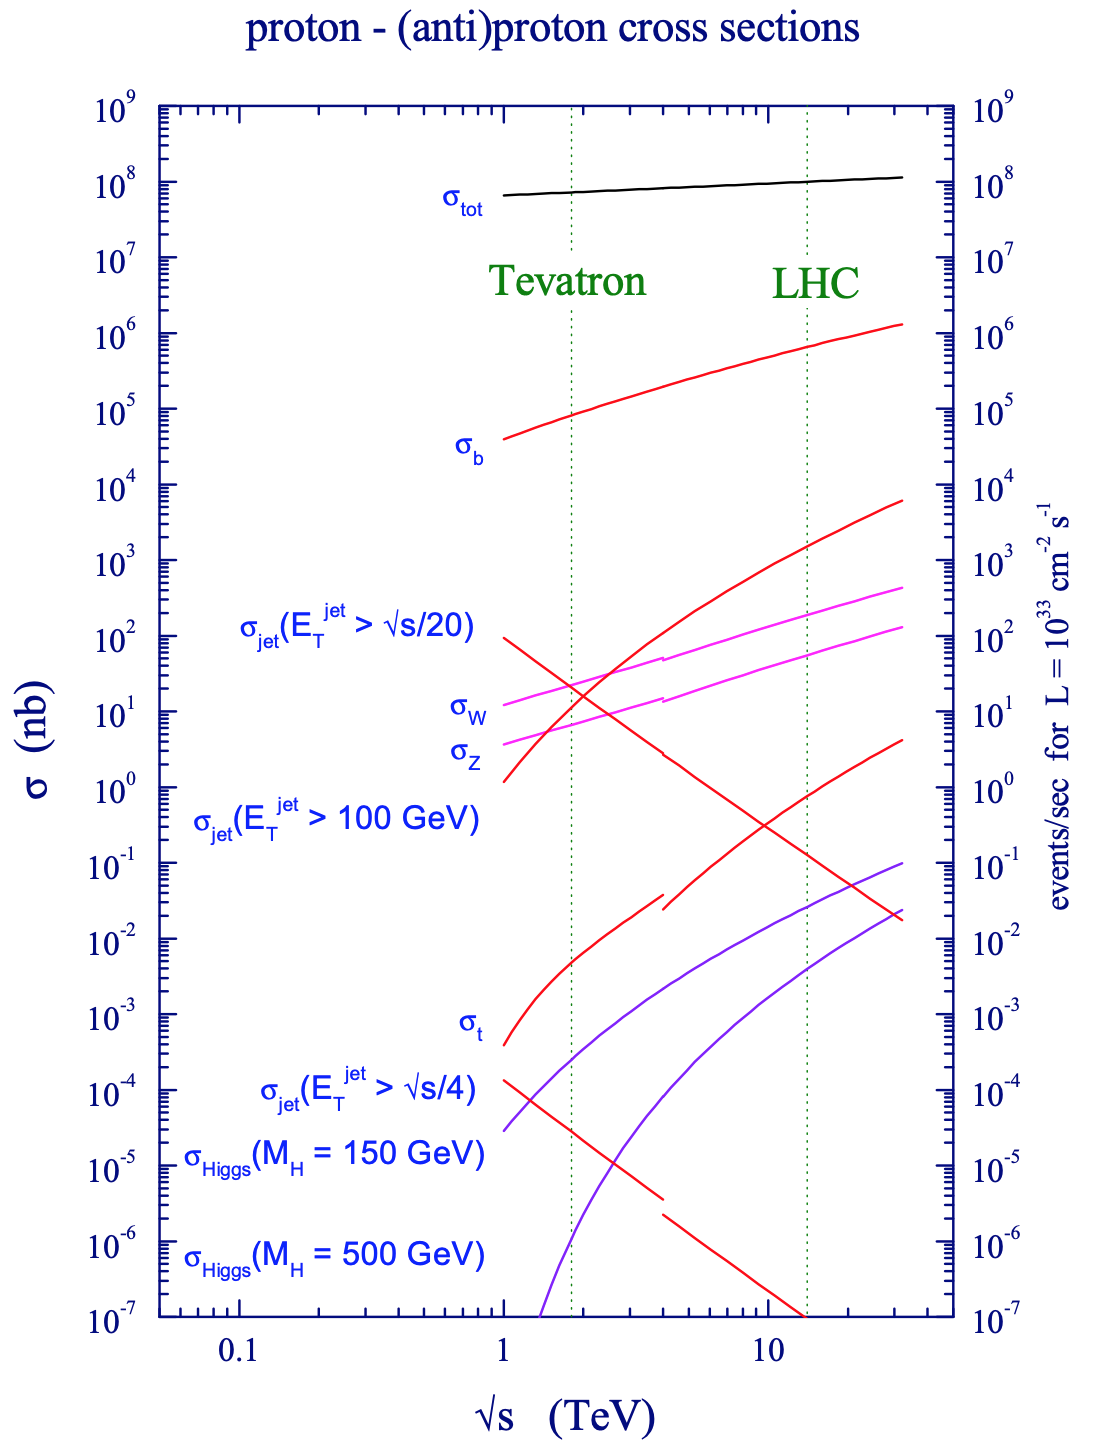
\includegraphics[width=0.6\linewidth]{figures/physics_of_pp/pp_cross_sections.png}
    \caption{Cross sections for typical processes of interest in pp collision experiments, shown as a function of the center-of-mass energy, $\sqrt{s}$. Taken from~\cite{Campbell:2006wx}.}
    \label{fig:pp_xs}
\end{figure}

\subsection{Parton Showers, Hadronization, and Jets} \label{sec:pp_physics_jets}
High energy processes involving the strong interaction are very well-described by perturbative QCD calculations.
However, at lower energies (less than or equal to about 1 GeV), the perturbative appraoch fails to provide an accurate description of the SM phenomena: the strong coupling $\alpha_s$ of QCD becomes close to unity, as shown in Fig.~\ref{fig:pp_qcd_coupling}.
\begin{figure} [htbp!]
    \centering
    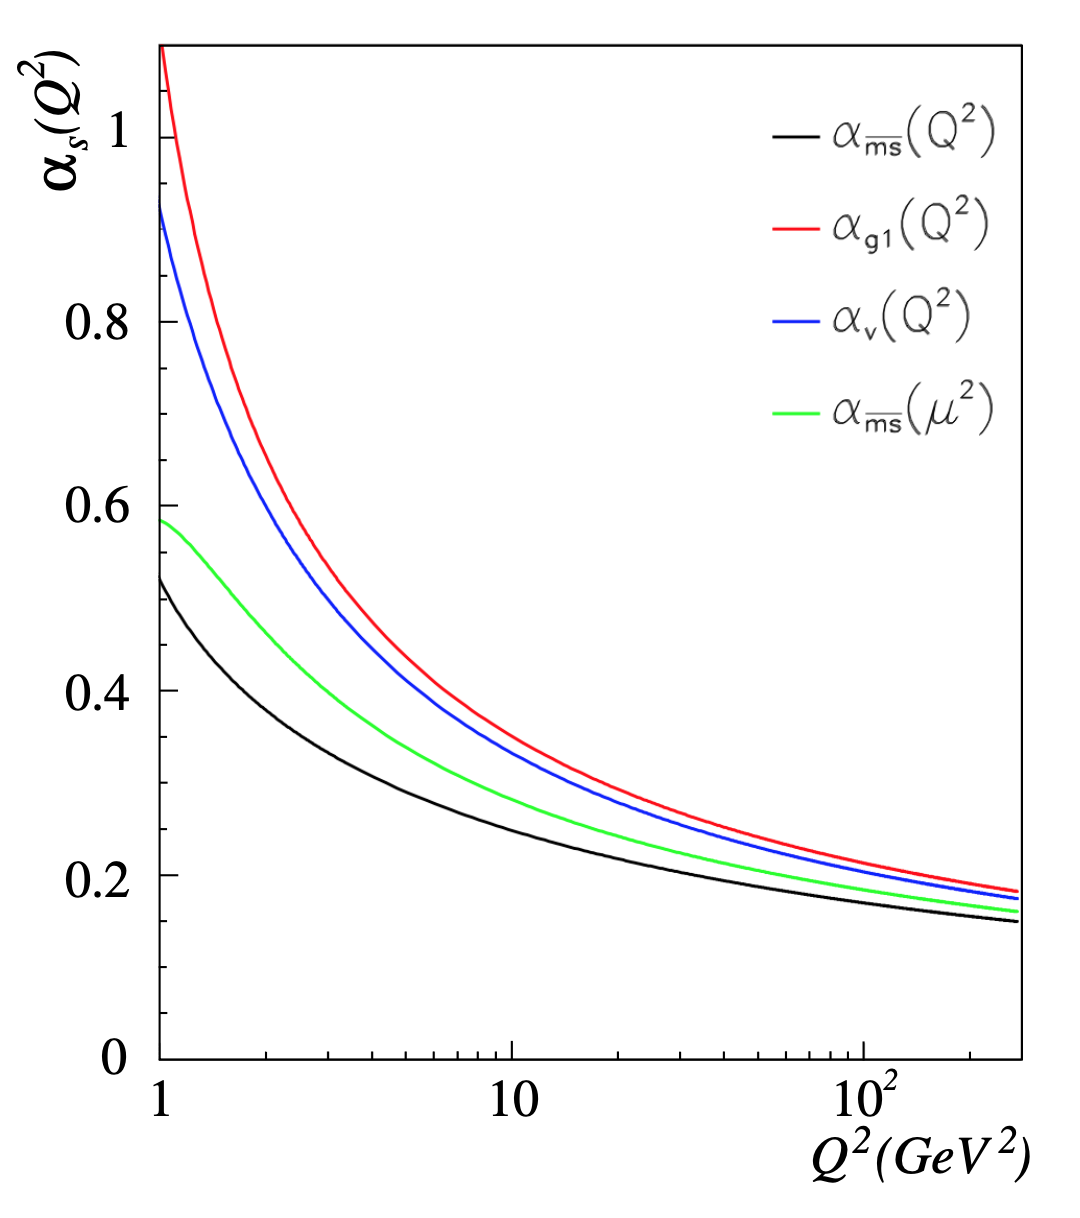
\includegraphics[width=0.6\linewidth]{figures/physics_of_pp/pp_qcd_coupling.png}
    \caption{The strong coupling constant $\alpha_s$ of QCD as a function of $Q^2$. Different colored lines correspond to various renormalization schemes. Taken from~\cite{Deur:2016tte}.}
    \label{fig:pp_qcd_coupling}
\end{figure}
When the coupling $\alpha_s$ nears unity, the perturbative approach fails for the following reason: perturbative expansions are made in powers of the coupling, so the coupling must be significantly less than one in order for a finite expansion to provide a good approximation.
In describing phenomena like parton showers and hadronization, energy scales of $\mathcal O(1)$ GeV are relevant, and a strictly perturbative calculation will not provide a satisfactory description.

A \emph{parton shower} refers to the process by which a high energy parton stemming from the hard interaction produce showers of ``soft'' particles at lower energies.
Typically, this is either gluon splitting, in which a gluon converts into a quark-antiquark pair, or gluon radiation, in which a quark radiates a gluon.
In practice, parton showers are modeled with Monte Carlo generators which utilize Sudakov form factors~\cite{Sudakov:1954sw} and splitting functions to simplify calculations~\cite{Hoche:2014rga}.

As discussed in Sec.~\ref{sec:theory_qcd}, quarks and gluons are confined to bound states which must be colorless.
Moreover, the potential energy of a hadron increases as a function of the distance between the partons.
At a large enough distance, it becomes energetically favorable to break the original bound state in which they existed and instead form new hadrons.
This process is called \emph{hadronization}.
In high energy collisions, quarks and gluons are often ejected from the hard interaction with high enough momentum for hadronization to occur. 
Frequently, the newly formed hadron will initiate a cascade of decays and gluon radiation, forming a cone of hadronic activity.
This cone of particles stemming from the hadronization of a quark or gluon is called a \emph{hadronic jet}.
Hadronization cannot be adequately described through perturbative calculations alone, and instead phenomenological models like the Lund-String Model~\cite{Andersson:1983ia} are employed.

\subsection{Underlying Event and Pileup}
In a given bunch crossing, there is typically only one hard scattering interaction of interest from a physics point of view.
In addition to this hard interaction, there are additional lower energy ``soft'' scattering interactions.
The soft scattering may be due either to interactions between partons other than those involved in the hard scattering interaction or interactions between protons other than those involved in the hard scattering interaction.
The former is called the \emph{underlying event}, while the latter interactions are called \emph{pileup} interactions.
The modeling of underlying event and pileup is often performed through heuristic approaches which extrapolate directly from experimental collision data.

Though soft scattering interactions from underlying event and pileup are typically not of interest, it is still imperative to understand and adequately model them in order to study physics processes of interest.
A large portion of the hadronic activity in an event at the LHC stems from these soft interactions and will effect, for example, the jet multiplicity and missing transverse momentum calculation in that event.
Physics analyses often use the jet multiplicity and missing transverse momentum to identify regions of high signal purity (for example, an analysis searching for supersymmetric particles will typically select for events with high missing transverse momentum) -- for these reasons, it is vital to understand the contribution of underlying event and pileup to these distributions in order to properly model the targeted signal process and accurately estimate the relevant SM background processes.

Parton showers, hadronization, and underlying event are visually depicted for a hadron-hadron collision in Fig.~\ref{fig:pp_event_schematic}.

\begin{figure} [htbp!]
    \centering
    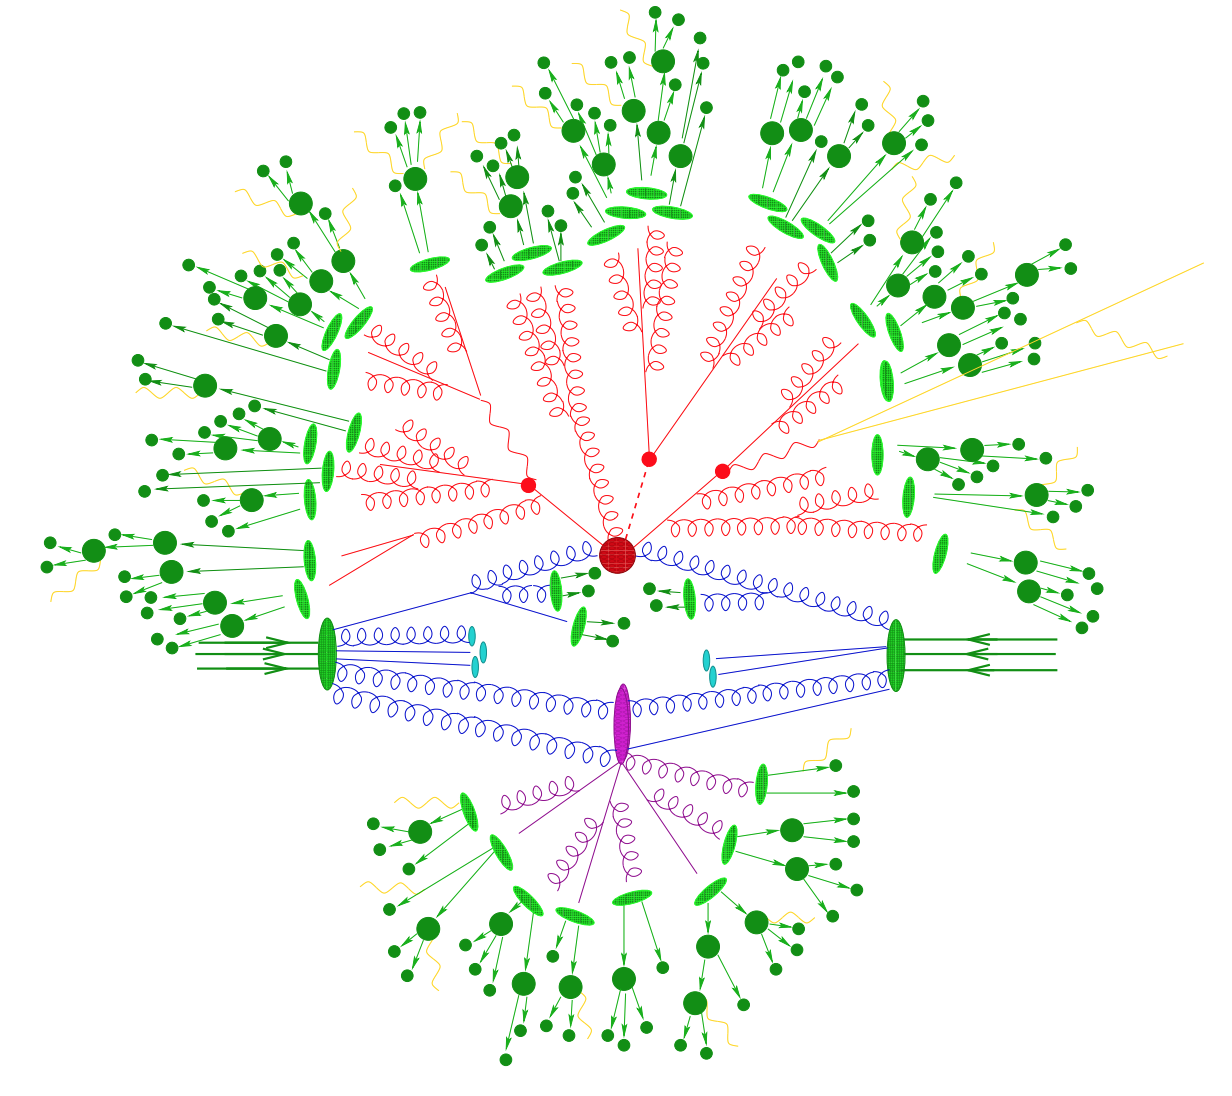
\includegraphics[width=0.7\linewidth]{figures/physics_of_pp/pp_event_schematic.png}
    \caption[Schematic of a hadron-hadron collision. Taken from~\cite{Hoche:2014rga}.]{Schematic of a hadron-hadron collision. The red blob indicates the hard scattering interaction and the subsequent tree-like structure depicts parton showers, while the purple blob indicates an underlying event scattering interaction. Light green blobs depict hadronization, dark green blobs depict subsequent decays of those hadrons, and yellow lines depict soft Bremsstrahlung radiation. Taken from~\cite{Hoche:2014rga}.}
    \label{fig:pp_event_schematic}
\end{figure}


\section{Monte Carlo Simulation} \label{sec:pp_mc}

The CMS detector was designed with two primary physics goals in mind.
First, to study the properties of the Higgs boson; in particular, the nature of electroweak symmetry breaking for which the Higgs mechanism is responsible\footnote{Note that during the design of the CMS detector, the Higgs boson was theorized to exist but had not yet been discovered.}.
Second, to reveal signs of physics beyond the Standard Model which might be present at the TeV scale.
This section discusses technical design aspects of the CMS detector and how they support the physics goals of the CMS experiment.
\subsection{General Design Concepts} \label{sec:cms_overview}
The CMS detector is over 20m in length and nearly 15m in diameter -- it is ``compact'' only in the context of the tremendous size of a detector needed to facilitate the physics goals for which it was designed.
The various components of the CMS detector are shown in Fig.~\ref{fig:cms_schematic}, with humans shown to illustrate the scale (banana not available).

\begin{figure} [htbp!]
    \centering
    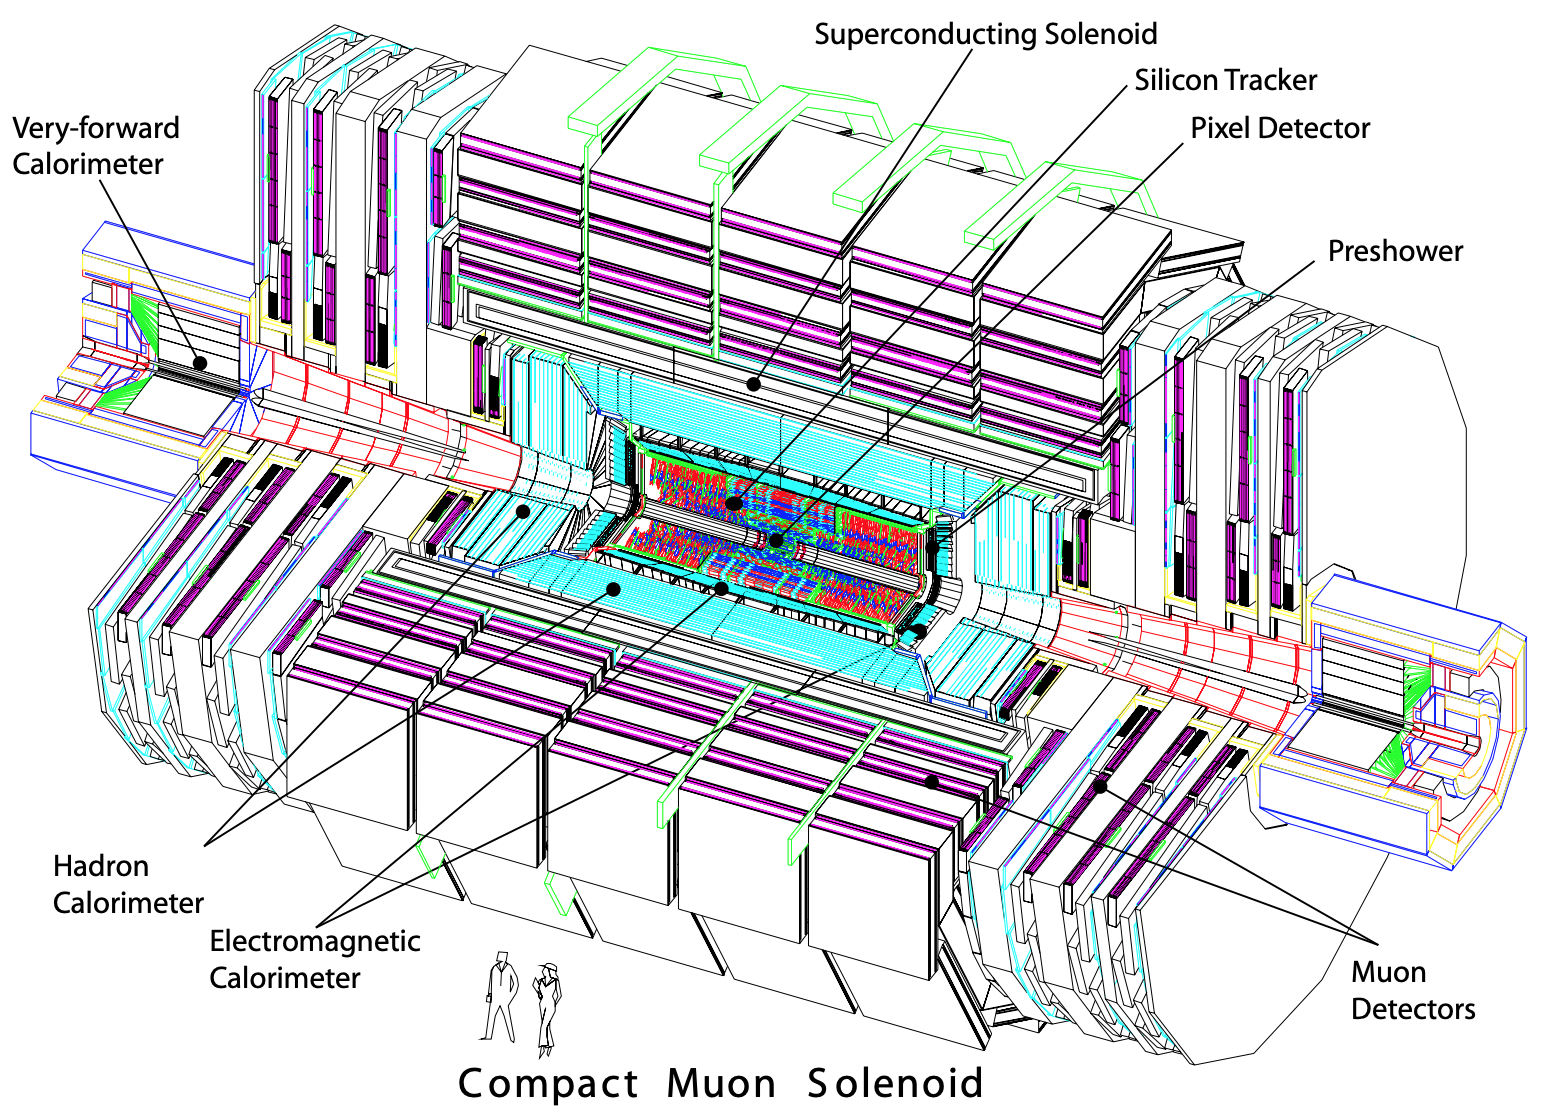
\includegraphics[width=0.8\linewidth]{figures/cms/cms_detector_schematic.png}
    \caption{Schematic of the various components of the CMS detector. Taken from~\cite{Chatrchyan:2008aa}.}
    \label{fig:cms_schematic}
\end{figure}

As its name suggests, the primary feature of the CMS detector is a superconducting solenoid providing a magnetic field of 4~T.
The purpose of the magnetic field is to bend the path of charged particles originating from inelastic proton-proton interactions: the precise spatial resolution of the tracker and muon system allows one to determine a particle's radius of curvature, in turn allowing one to determine the particle's momentum.
Excellent momentum resolution of charged particles supports nearly every physics analysis performed with the CMS detector, but is especially important for determining the invariant mass of heavy resonances (e.g. studying the properties of the Higgs boson in the H $\to$ ZZ$^{*} \to 4l$ channel), distinguishing between hadronic jets which originate from b quarks from those which originate from gluons or light-flavor quarks (e.g. the H $\to$ bb decay channel and searches for new physics involving final states with b-jets), and for precise resolution of the missing transverse energy (e.g. final states with neutrinos or searches for new physics involving final states with undetected dark matter or supersymmetry candidate particles).

The other major components of the detector include: 
\begin{itemize}
    \item The tracker, which allows for identification and measurement of the momenta of charged particles.
    \item The electromagnetic calorimeter (ECAL), which allows for identification and momenta measurement of electrons and photons, particularly important for H $\to \gamma \gamma$ physics.
    \item The hadronic calorimeter (HCAL), which assists in the identification and momentum resolution of charged hadrons and provides the only handle on measuring neutral hadrons.
    \item The muon system, which enables better momentum resolution of very high energy ($\mathcal O$(TeV)) muons (while the tracker excels in providing good momentum resolution for lower energy, $\mathcal O$(GeV) muons).
\end{itemize}
Each of these components is described in greater detail in the following subsections.

A design consideration common to multiple subdetector components is the goal of hermeticity: a fully hermetic detector is able to measure particles emerging in any direction from an inelatic collision.
In other words, a hermetic detector has full coverage of the $4\pi$ steradians of solid angle surrounding the interaction point.
The CMS detector is not fully hermetic, as it is practically impossible to measure particles which emerge parallel to the LHC's proton beams.
Still, the CMS detector is able to measure very forward particles (with ``forward'' meaning ``close to parallel with the beam axis''), aiding the nearly complete reconstruction of the final state of a given pp interaction, which is essential for resolution of the missing transverse energy.

To expand upon the concepts of hermeticity and the identification of forward particles, we must first introduce the coordinate system used to describe the CMS detector.
Given the cylindrical shape of the detector, standard cylincdrical coordinates form the basis of the coordinate system: the $\hat{z}$-axis is defined as the axis along which the proton beams travel, and the $\hat{\phi}$ direction then coincides with the detector's circular symmetry perpendicular to the beam axis.
Instead of the typical polar angle $\hat{\theta}$, position is usually expressed in terms of pseudorapidity, defined in terms of $\theta$ as
\begin{equation}
    \eta = -\ln \Bigg[ \tan \bigg(\frac{\theta}{2}\bigg) \Bigg].
\end{equation}
A pseudorapidity of $\eta = 0$ corresponds to a direction perpendicular to the beam axis, while $\eta = \infty$ corresponds to a direction parallel to the beam axis.
Pseudorapidity is convenient for a number of reasons, including the fact that it is nearly Lorentz invariant under boosts along the $\hat{z}$-axis.
We say that it is ``nearly'' Lorentz invariant as this is only true for massless particles.
However, at the LHC, the transverse momentum of a given particle is typically sufficiently larger than the mass ($\pT >> m$) such that the pseudorapidity is approximately Lorentz invariant. 

Much of the reason for CMS's 20m of length in the direction of the beam axis is motivated by the goal of hermeticity.
The forward calorimeter (described in greater detail in Sec.~\ref{sec:cms_hcal}) provides coverage up to pseudorapidities of $|\eta| \leq 5.0$.
Pairing the extensive range in pseudorapidities with the CMS detector's complete coverage in the $\hat{\phi}$-direction, the CMS detector is nearly hermetic, aiding the resolution of missing transverse energy and consequently the ability to infer the presence of undetected particles.
The exact coverage of each of the detector subcomponents is discussed in greater detail in the following subsections.

\subsection{Solenoid}
The solenoid installed in the CMS detector is over 12~m in length and 6m in diameter, capable of providing a 4~T magnetic field.
The purpose of such a strong magnetic field is to bend the trajectories of charged particles (as illustrated in Fig.~\ref{fig:cms_transverse_view}, allowing CMS to measure their momentum, mass, and charge.
Fig.~\ref{fig:cms_transverse_view} depicts the three major classes of particles which have their trajectories curved by the magnetic field produced by the solenoid: an electron (red), a charged hadron (green), and a muon (blue).
Measurements of the momenta of electrons are also aided by the ECAL (described in Sec.~\ref{sec:cms_ecal}), those of charged hadrons are also aided by the HCAL (described in Sec.~\ref{sec:cms_hcal}), and those of muons are also aided by the muon system (described in Sec.~\ref{sec:cms_muon_system}).

\begin{figure} [htbp!]
    \centering
    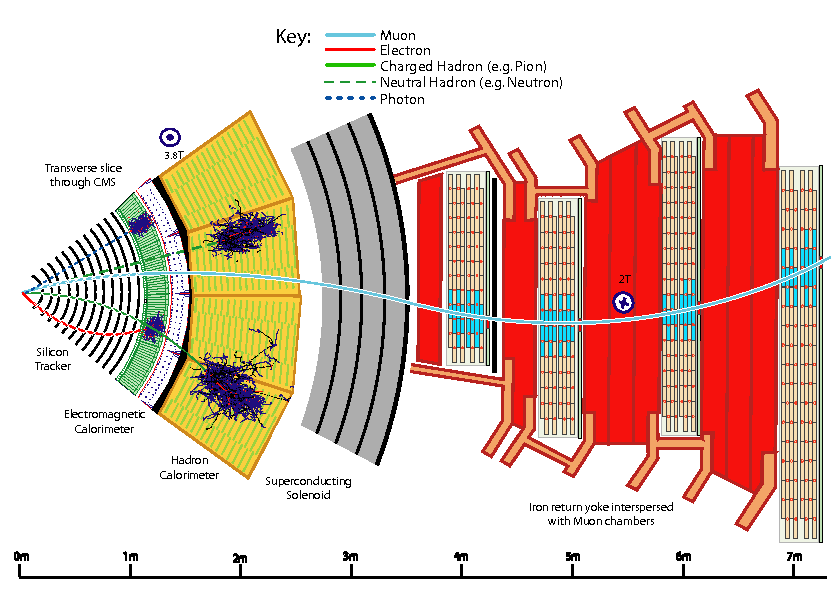
\includegraphics[width=\linewidth]{figures/cms/cms_transverse_view.png}
    \caption{Depiction of a transverse slice of the CMS detector, along with trajectories of particles of different types. Taken from~\cite{Sirunyan:2270046}.}
    \label{fig:cms_transverse_view}
\end{figure}

The solenoid is installed around the the tracker (Sec.~\ref{sec:cms_tracker}), the ECAL (Sec.~\ref{sec:cms_ecal}), and the HCAL (Sec.~\ref{sec:cms_hcal}) which is why the solenoid must be so large.
In order to support the massive current (over $10^4$~A) required for the magnetic field, the solenoid is constructed with superconducting Niobium-Titanium (NbTi), and its temperature must be kept sufficiently low to ensure superconductivity of the NbTi. 

\subsection{Tracker} \label{sec:cms_tracker}
The innermost component of the CMS detector is the silicon tracker, and its primary aim is to provide the precise reconstruction of charged particles and secondary vertices (an inelastic pp collision is deemed a ``primary vertex'' while decays of particles produced from a primary vertex are deemed ``secondary vertices'').
The tracker is nearly 6~m in length and 2.5~m in diameter, composed of an inner pixel detector with three layers ranging from 4-10~cm and an outer silicon strip tracker with ten layers ranging to 1.1~m.
Both the pixel detector and the silicon strip tracker are accompanied by endcap disks on either end of the barrel, extending the pseudorapidity coverage to $|\eta| \leq 2.5$.
Between the data-taking periods corresponding to 2016 and 2017, the inner pixel detector was upgraded~\cite{Botta:2285433}, extending the coverage of the tracker up to $|\eta| \leq 3.0$.
As shown in Fig.~\ref{fig:cms_tracker_upgrade}, the number of fake tracks, the impact parameter resolution, and the vertex resolution are each improved as well, resulting in an approximately 10\% improvement in the b-tagging efficiency for a fixed fake rate.

\begin{figure} [htbp!]
    \centering
    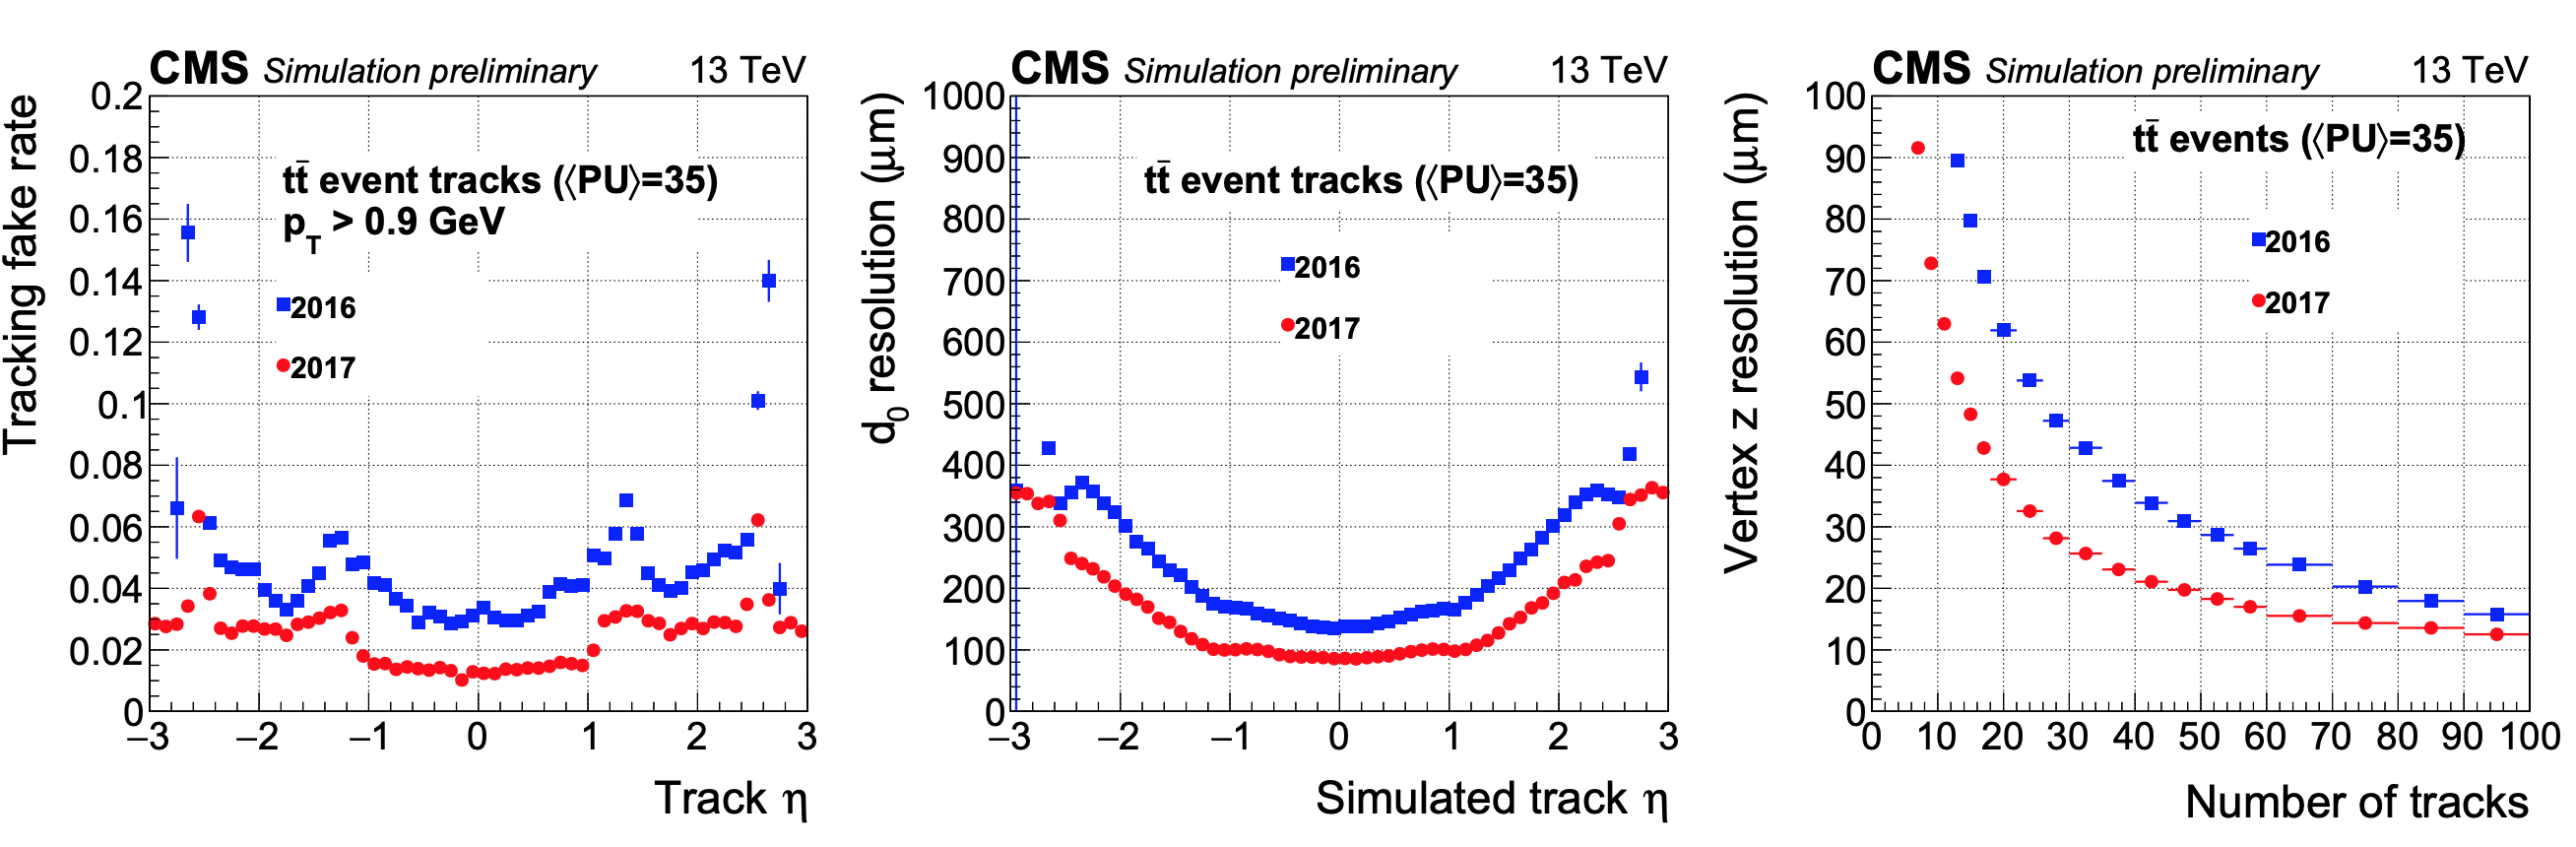
\includegraphics[width=\linewidth]{figures/cms/cms_pixel_upgrade.png}
    \caption{Comparison of tracker performance before and after the upgrade to the pixel detector, performed in between the 2016 and 2017 data-taking periods. Taken from~\cite{Botta:2285433}.}
    \label{fig:cms_tracker_upgrade}
\end{figure}

The primary design considerations for the tracker include the following:
\begin{itemize}
    \item Ability to reconstruct a large number of charged particles in each bunch crossing, with $\mathcal O(1000)$ charged particles expected from a single bunch crossing at the LHC design luminosity of $\mathcal L = 10^{34}$~cm$^{-2}$~s$^{-1}$ (corresponding to about 20 individual pp interactions).
    \item Ability to reconstruct charged particles with precise temporal resolution, with bunch crossings separated by a distance corresponding to 25~ns.
    \item Minimal interaction of photons with the tracker material, as precise measurements of photons are vital to studying Higgs physics in the \Hgg decay channel.
\end{itemize}

The first two considerations are in direct conflict with the third consideration: a tracker with high granularity and fast response implies large power density of electronics, which requires efficient cooling. This increases the material budget of the tracker, increasing the chances of bremsstrahlung and photon conversions, which in turn degrade the ECAl's photon energy resolution. 
An acceptable compromise providing both execllent tracking and excellent photon resolution was achieved with the tracker design depicted in Fig.~\ref{fig:cms_tracker_schematic}.

\begin{figure} [htbp!]
    \centering
    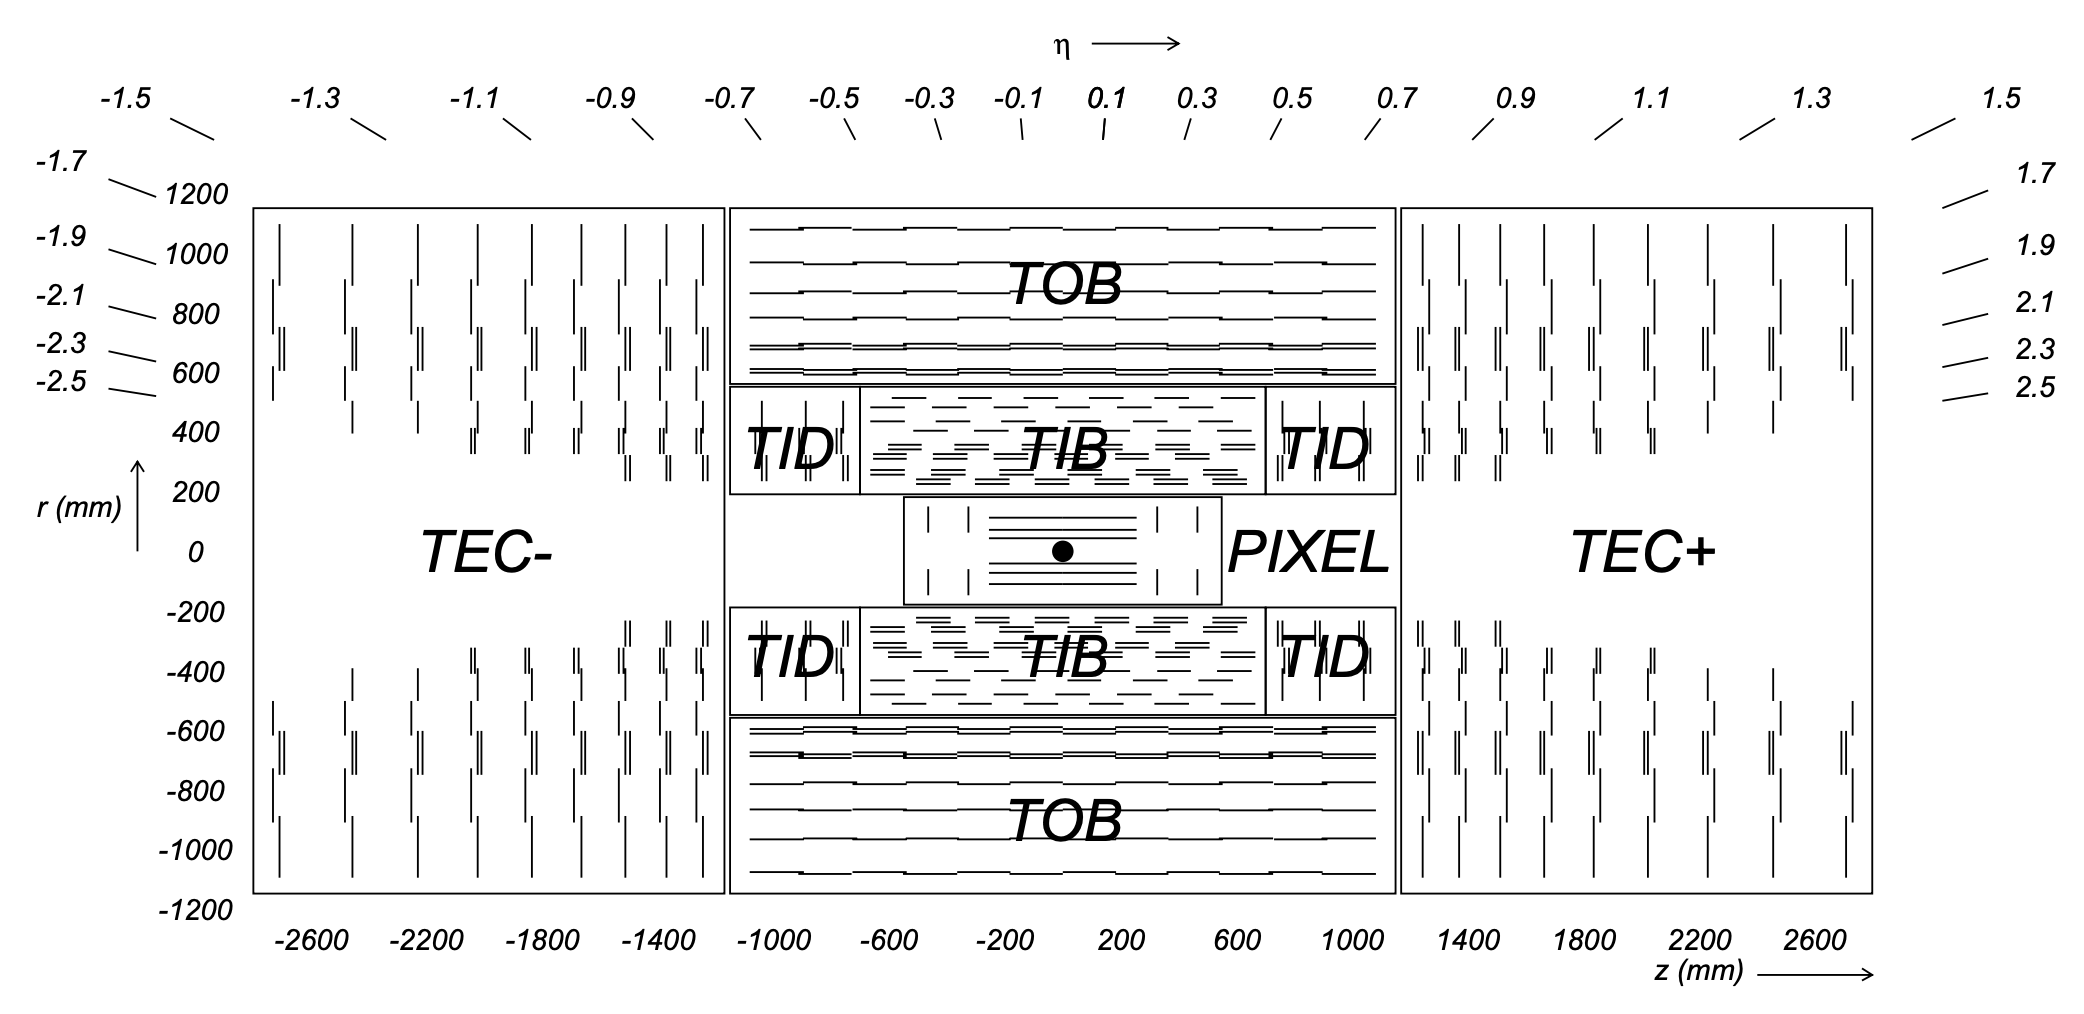
\includegraphics[width=0.8\linewidth]{figures/cms/cms_tracker_schematic.png}
    \caption{Schematic of the CMS tracker from a cross-sectional viewpoint. TIB, TOB, TID, and TEC represent the tracker inner barrel, tracker outer barrel, tracker inner disk, and tracker endcap components, respectively. Taken from~\cite{Chatrchyan:2008aa}.}
    \label{fig:cms_tracker_schematic}
\end{figure}

The material budget for the CMS tracker is shown in Fig.~\ref{fig:cms_tracker_budget}, showing the thickness of the tracker material in terms of the characteristic radiation lengths $X_0$ (for electromagnetic particles, e.g. electrons and photons) and characteristic nuclear interaction lengths $\lambda_I$ (i.e. for hadrons).
The tracker thickness in terms of both radiation lengths and nuclear interaction lengths is lowest in the most central part of the barrel and increases in the more forward components, accounting for one of the reasons that CMS achieves better energy resolution for very central particles.

\begin{figure} [htbp!]
    \centering
    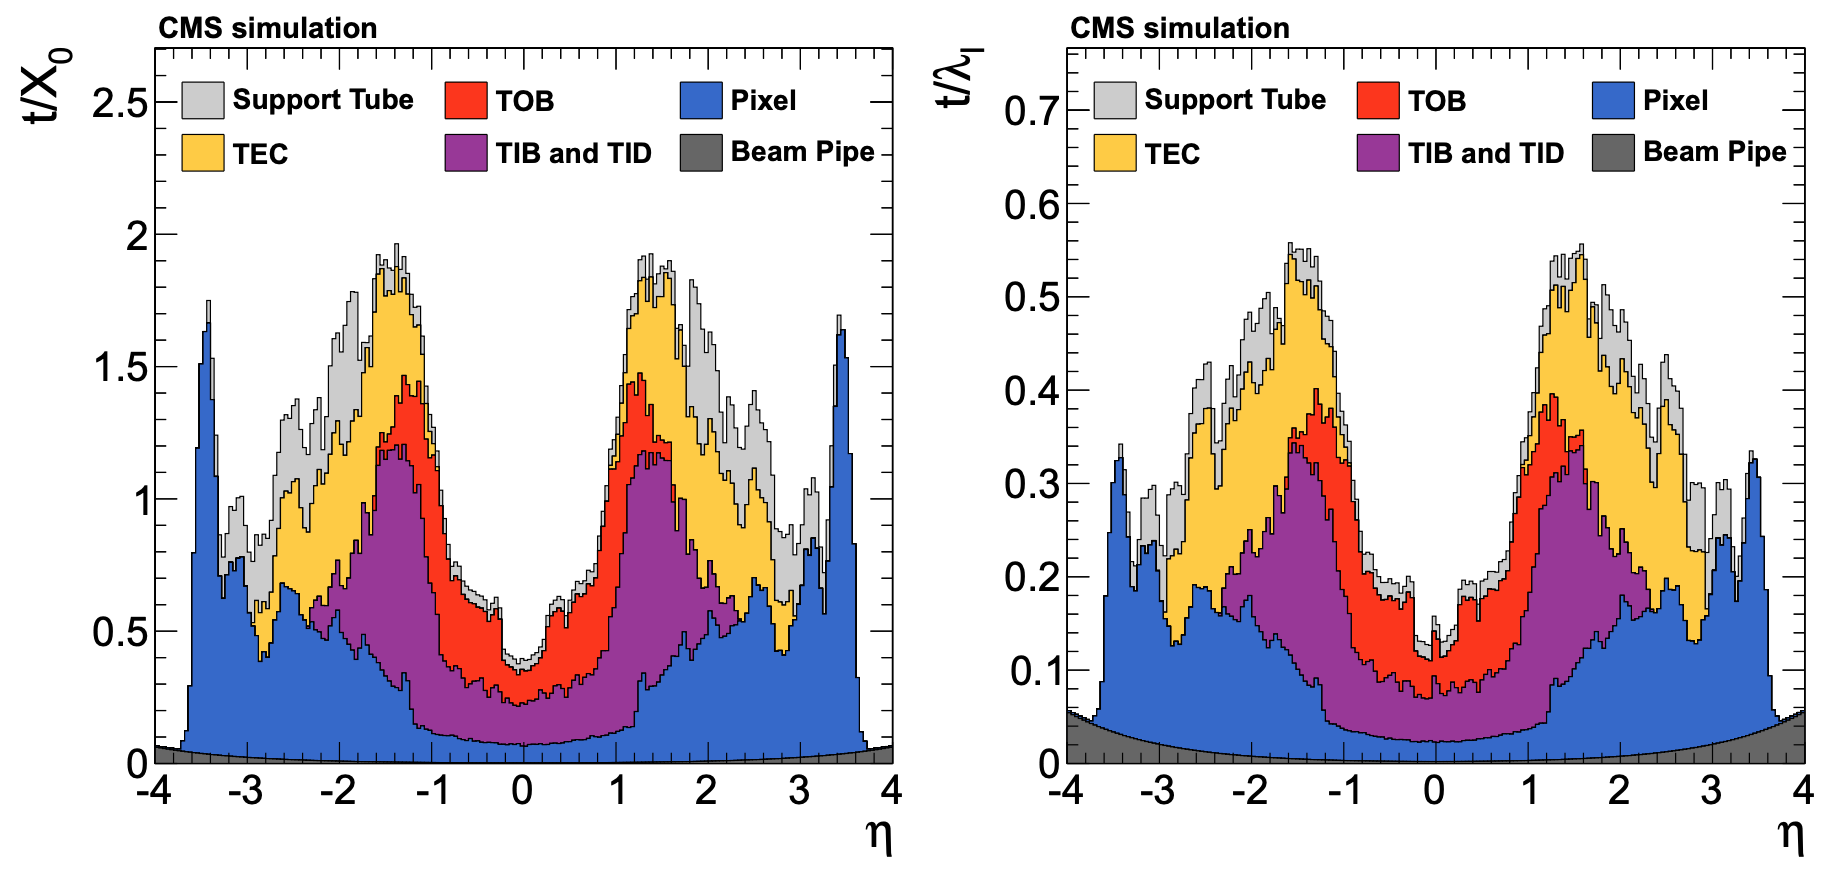
\includegraphics[width=\linewidth]{figures/cms/cms_tracker_budget.png}
    \caption{The material budget for the CMS tracker shown for both the characteristic radiation lengths of electromagnetic interactions (left) and the characteristic nuclear interaction lengths of hadronic interactions (right), with the contributions of each of the tracker subcomponents shown individually. Taken from~\cite{Chatrchyan:1704291}.}
    \label{fig:cms_tracker_budget}
\end{figure}

The tracking effieciency achieved by the CMS tracker is shown in Fig.~\ref{fig:cms_tracker_eff}, for muons, pions, and electrons as a function of their transverse momentum.
In general, the tracker achieves higher efficiency for muons than for electrons or pions, as electrons are more likely to emit radiation via bremsstrahlung and charged pions may undergo nuclear interactions with the tracker material.
Energy resolution of high \pT ($\mathcal O(TeV)$) muons is assisted by the muon system, as shown in Fig.~\ref{fig:cms_muon_vs_tracker}.

\begin{figure} [htbp!]
    \centering
    \begin{tabular}{c c c}
        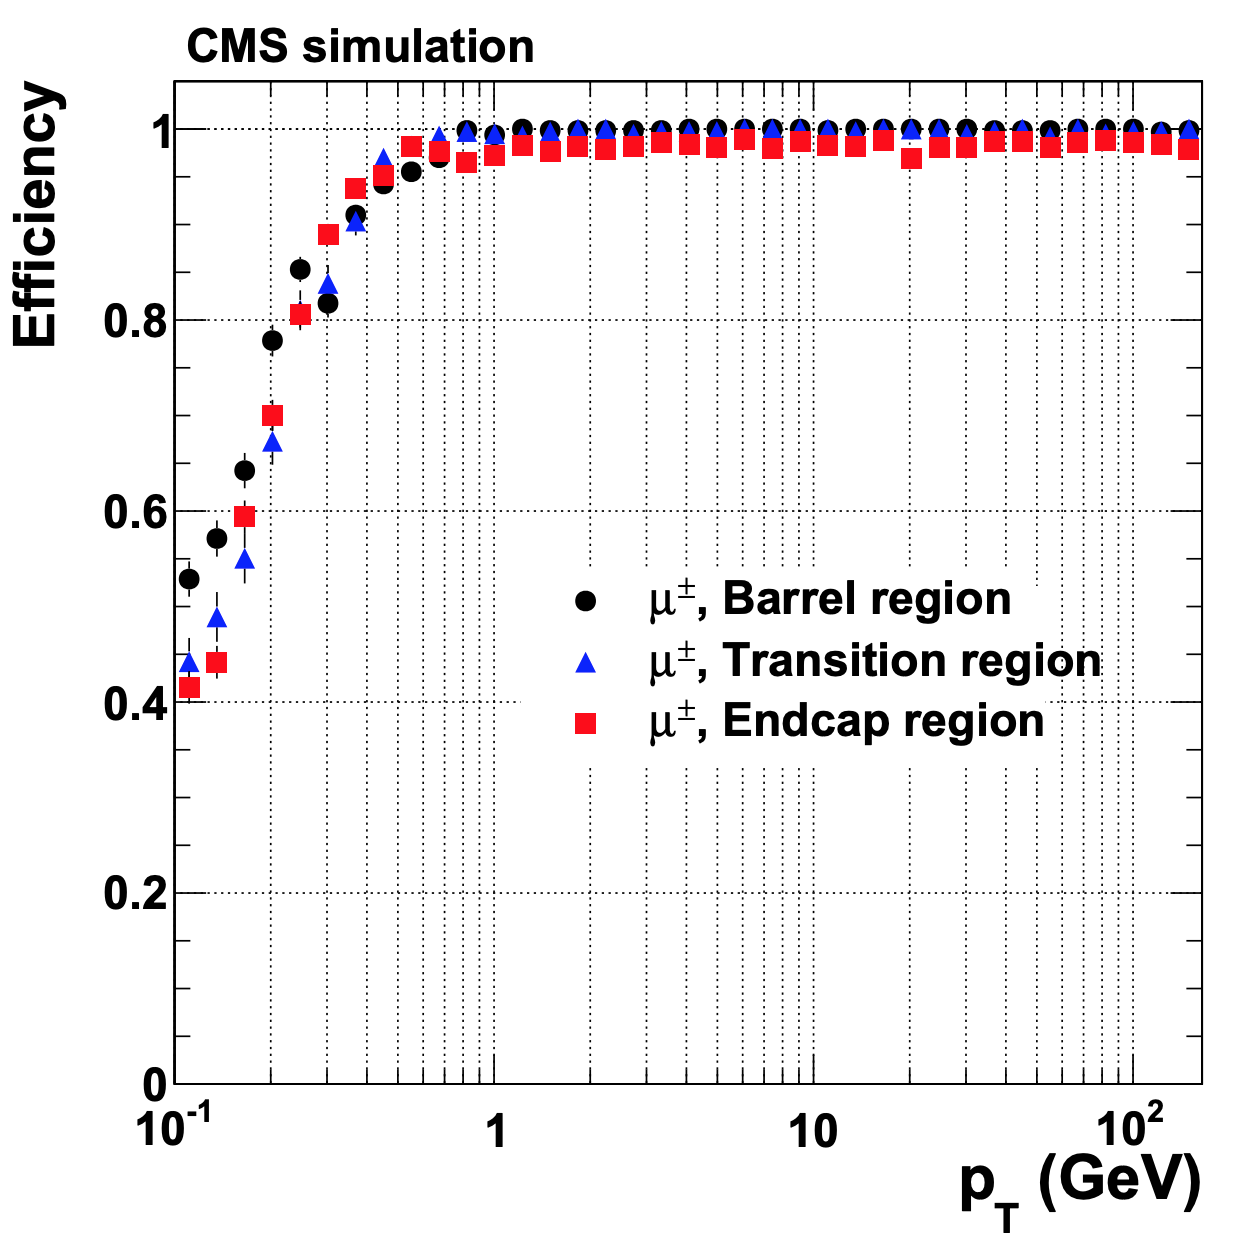
\includegraphics[width=0.31\linewidth]{figures/cms/cms_tracker_muon.png} &
        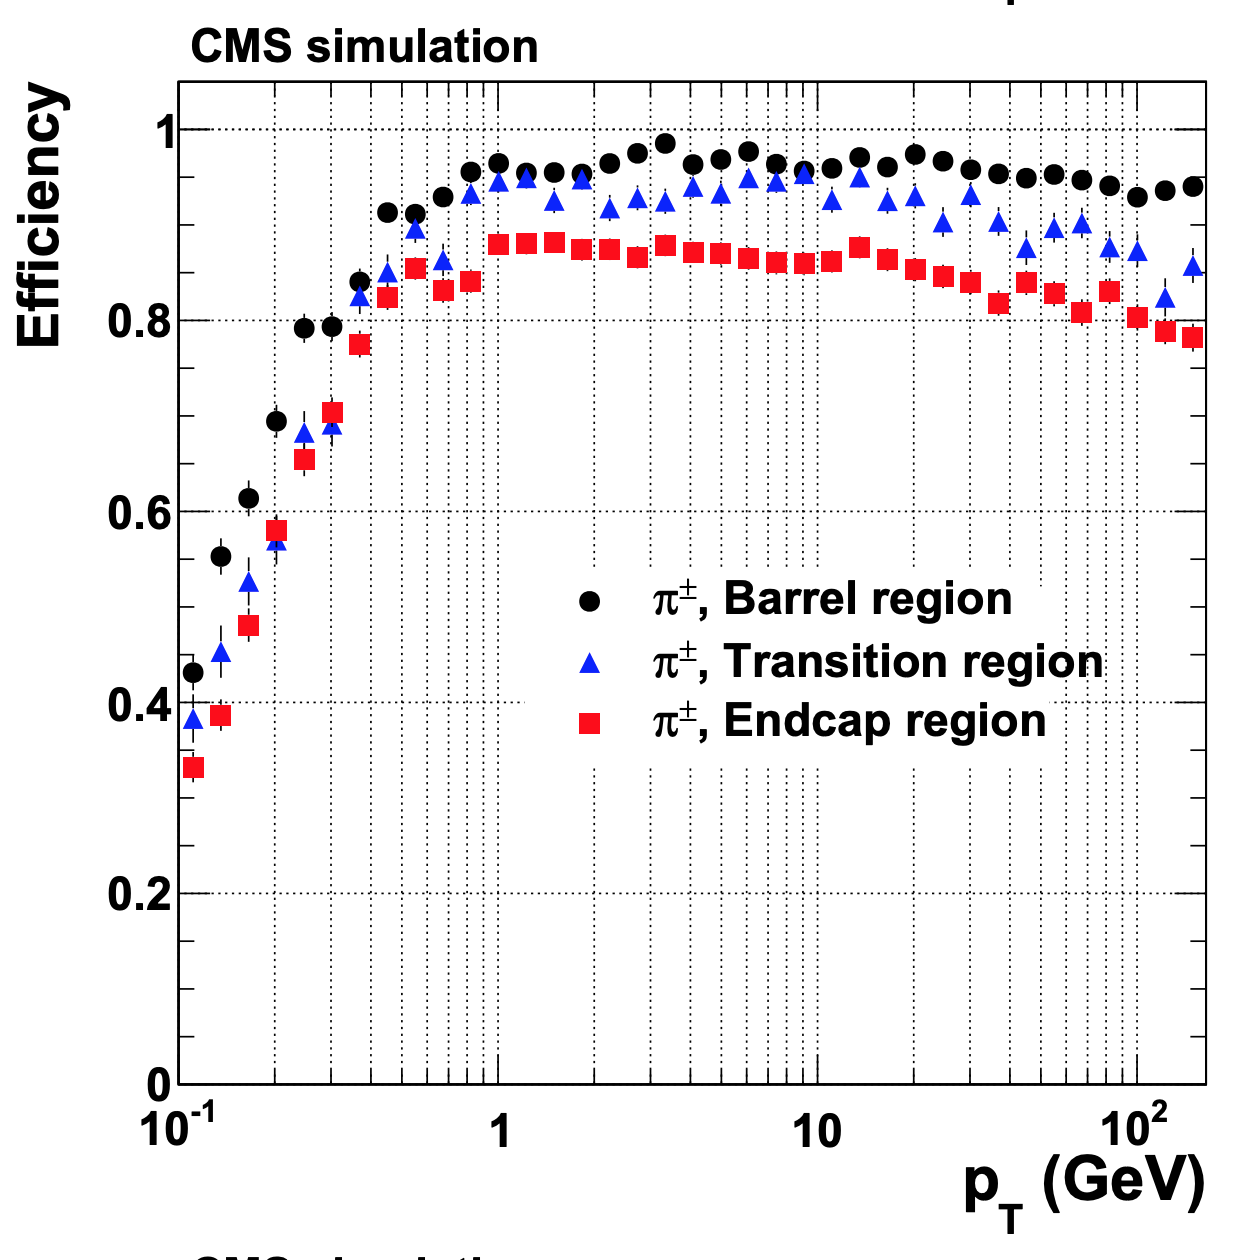
\includegraphics[width=0.31\linewidth]{figures/cms/cms_tracker_pion.png} &
        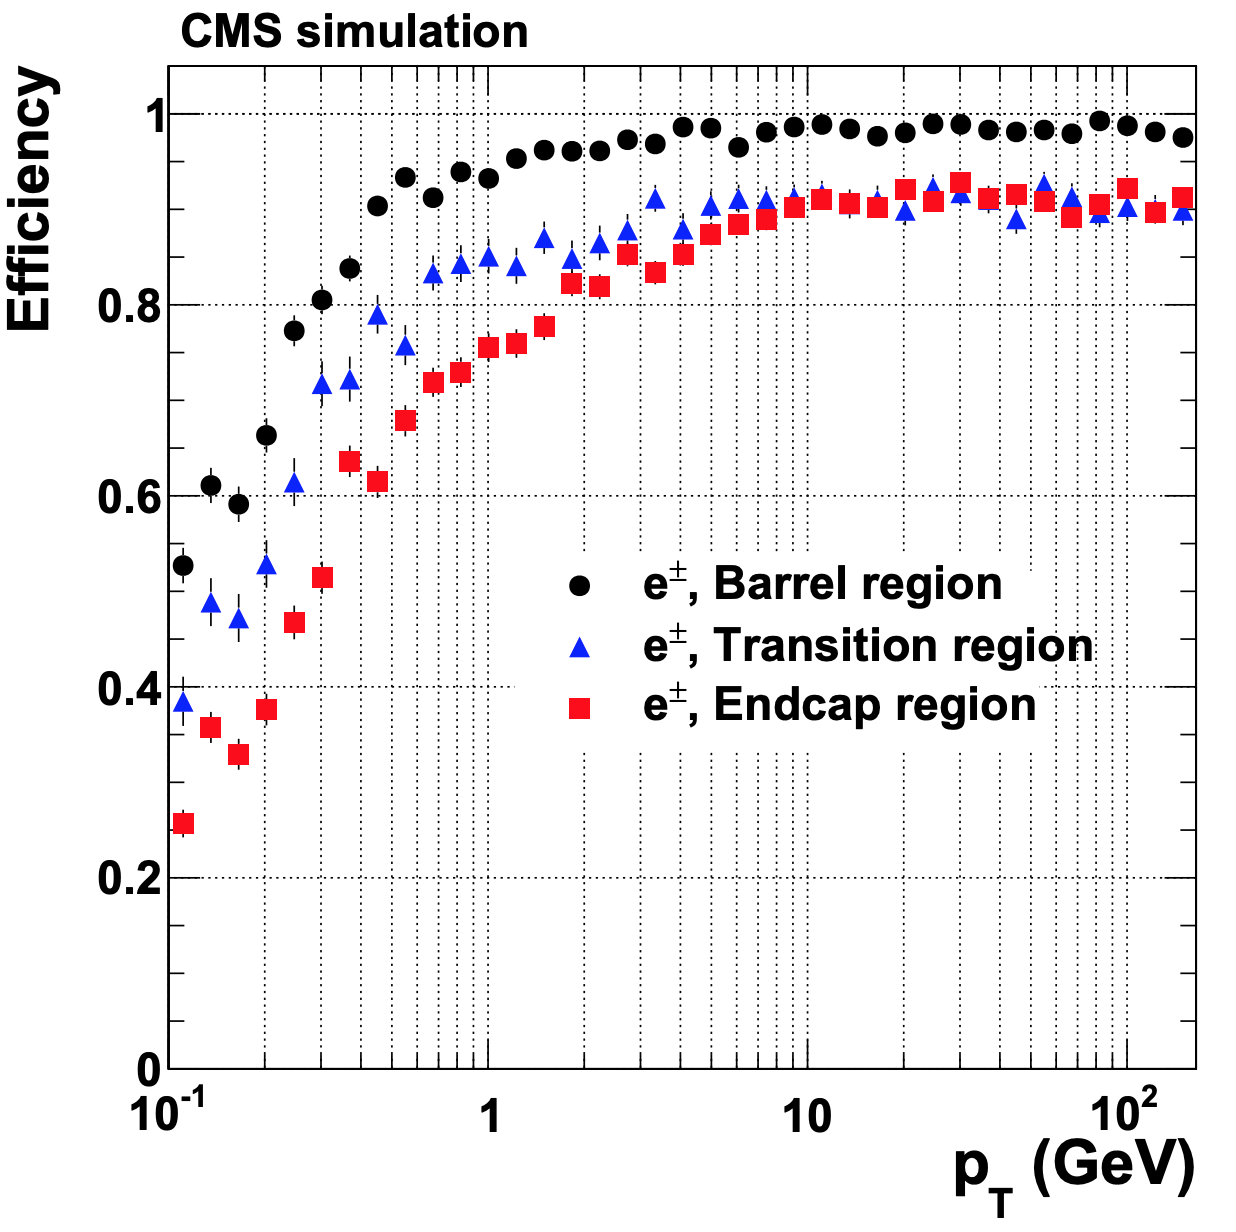
\includegraphics[width=0.31\linewidth]{figures/cms/cms_tracker_electron.png}
    \end{tabular}
    \caption{Tracking efficiency as a function of \pT for muons (left), charged pions (middle), and electrons (right), shown separately for the barrel (black), transition region (blue), and endcap (red). Taken from~\cite{Chatrchyan:1704291}.}
    \label{fig:cms_tracker_eff}
\end{figure}


\subsection{Electromagnetic Calorimeter} \label{sec:cms_ecal}
The primary goal of the CMS electromagnetic calorimeter is to preicsely measure the momenta of photons, especially important for studying the properties of the Higgs boson in the \Hgg channel.
Along with the tracker, the ECAL also assists in measurements of electrons which radiate a significant fraction of their energy through via bremsstrahlung as they pass through the detector.
Other charged particles, like charged pions and muons, interact relatively negligibly with the ECAL, as they emit a much smaller fraction of their energy via bremsstrahlung (due to the fact that they are much more massive than electrons).

The CMS ECAL is composed of over $6 \times 10^4$ lead tungstate (PbWO$_4$) crystals in the barrel and over $7 \times 10^3$ crystals in each of the endcaps, with the barrel component (EB) providing coverage up to $|\eta| \leq 1.479$ and the endcap components providing coverage from $1.479 \leq |\eta| \leq 3.0$~\cite{Chatrchyan:2008aa}.

Lead tungstate is an attractive choice for the ECAL crystals for several reasons, including its high density (8.28~g/cm$^3$), short radiation length (0.89~cm), and small Moliere radius (2.2~cm), defined as the average size of a cylinder containing 90\% of an incident photon or electron's energy.
The short radiation length allows the CMS ECAL to be compact, and the small Moliere radius allows for better spatial resolution of incident photons and electrons.
The former is important from a practical and financial point of view, as the ECAL must be placed within the HCAL and solenoid, while the latter is important as better spatial resolution allows for better diphoton and dielectron invariant mass resolution (assisting with idenitfying \Hgg and \Zee events).

Two additional attractive properties of lead tungstate include its short scintillation time and resistance to radiation damage.
The scintillation time must be on the order of the bunch crossing time at the LHC (25~ns) so that ECAL deposits from consecutive crossings can be distinguished from each other (a short bunch crossing time is desirable as it results in increased integrated luminosity).
Indeed, about 80\% of light is emitted within 25~ns within the CMS ECAL~\cite{Bayatian:2006nff}, allowing for high temporal resolution in the high luminosity conditions of the LHC.
Due to the high particle flux, radiation damage to detector components is inevitable; this results in wavelength-dependent loss of light transmission~\cite{Bayatian:2006nff}.
Although lead tungstate is particularly radiation-hard, the damage must still be tracked and corrected for by injecting laser light and monitoring the transparency of crystals.

Further details of the reconstruction of photons are described in Sec.~\ref{sec:evt_photon}.

\subsection{Hadronic Calorimeter} \label{sec:cms_hcal}
The CMS Hadronic Calorimeter (HCAL) is particularly important for measuring the momenta of neutral hadrons, the only detector subcomponent which is able to do so.
It also assists in the momenta measurements of charged hadrons, though the tracker is typically much more effective for this purpose.
Precisely measuring the momenta of hadrons allows for good energy resolution of hadronic jets -- this is important for constructing a reliable estimate of the missing transverse momentum in a given event.
Conversely, poor resolution of jet energies would result in poor resolution of the missing transverse momentum, degrading the experiment's ability to identify events in which there is true missing transverse momentum, either from neutrinos or yet-to-be discovered particles which do not interact with the CMS detector.
The CMS detector is typically able to achieve a mometum resolution of around 10\%~\cite{Bayatian:2006nff} for hadronic jets, using a combination of information from the various detector subcomponents.

The CMS HCAL is composed of two primary components: barrel (HB), covering $|\eta| \leq 1.4$ and endcap (HE), covering $1.3 \leq |\eta| \leq 3.0$.
The barrel component also contains a ``tail catcher'' placed outside the solenoid (HO), which covers up to $|\eta| \leq 1.26$.
Finally, a forward calorimeter (HF) specializes in measuring very forward particles, up to $|\eta| \leq 5$~\cite{Bayatian:2006nff}.
The various components of the HCAL and their pseudorapidity coverage are depicted in Fig.~\ref{fig:cms_hcal_schematic}.

\begin{figure} [htbp!]
    \centering
    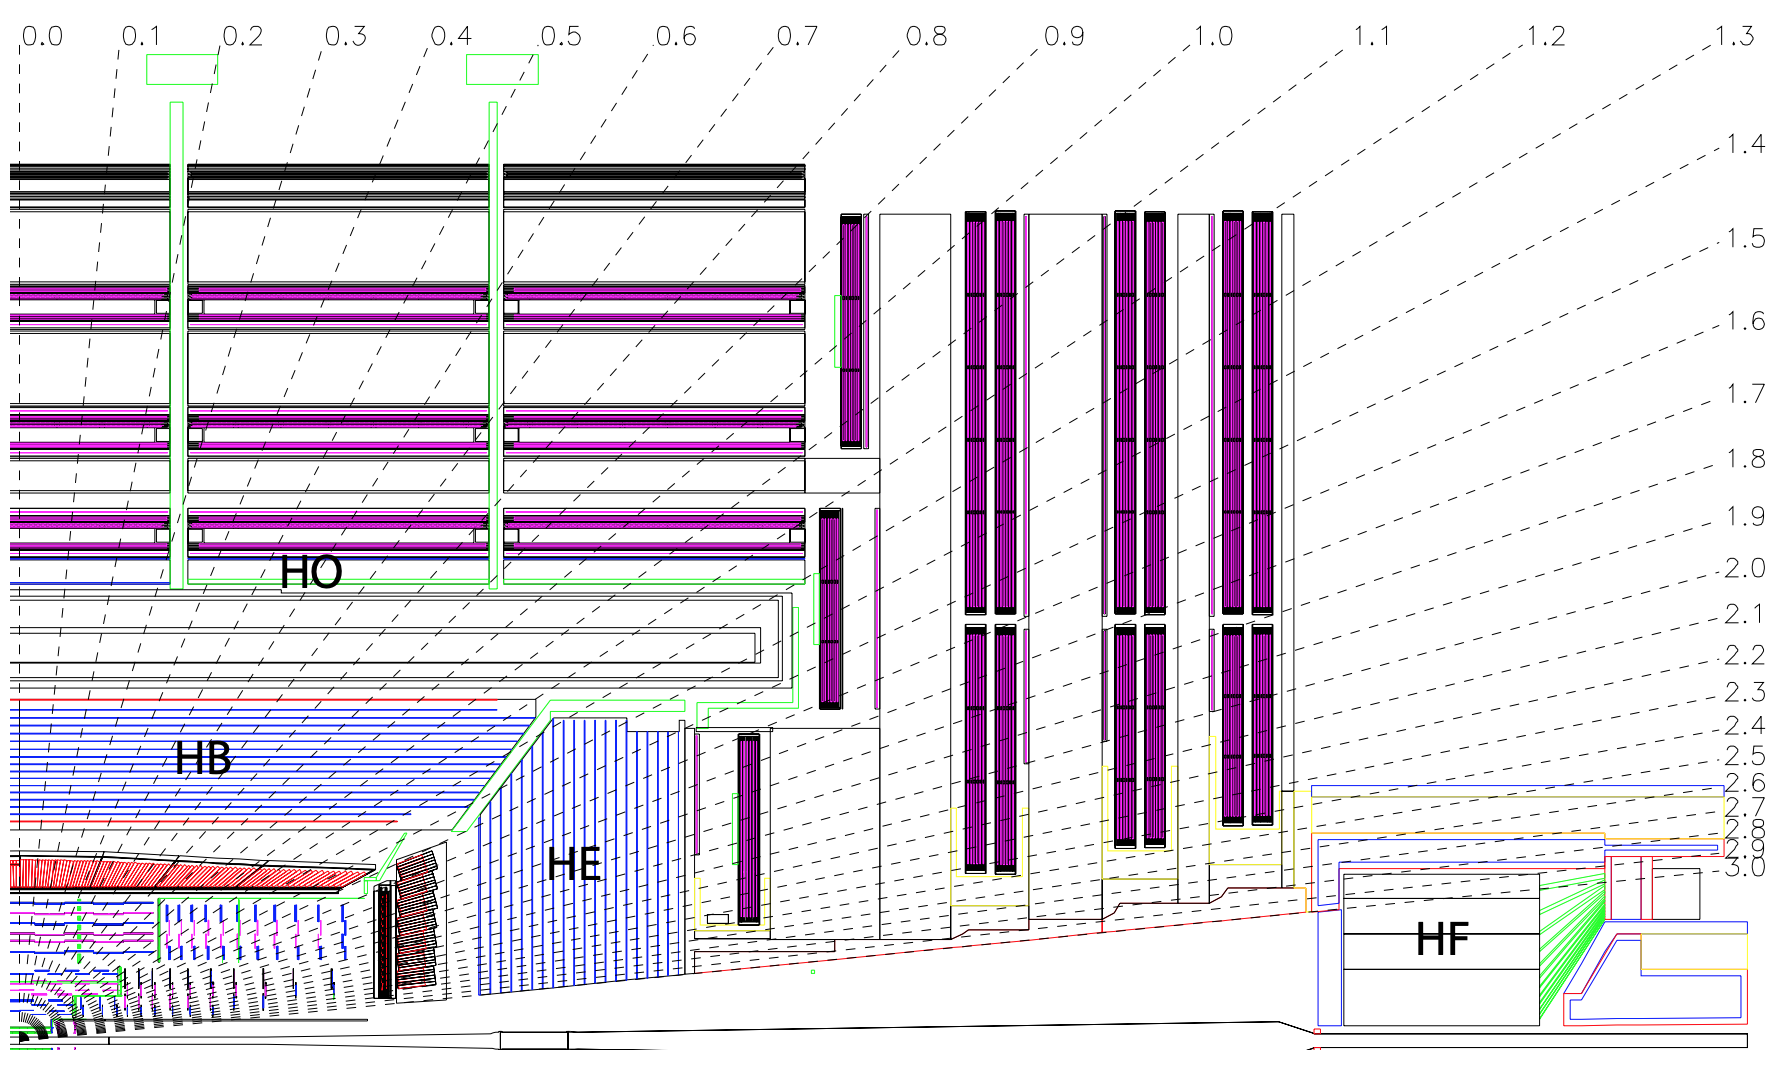
\includegraphics[width=0.7\linewidth]{figures/cms/hcal_schematic.png}
    \caption{Schematic of subcomponents of the CMS HCAL, along with their pseudorapidity coverage. Taken from~\cite{Chatrchyan:2008aa}.}
    \label{fig:cms_hcal_schematic}
\end{figure}

Conceptually, the HCAL aims to measure hadron energies by placing a high density of atomic nuclei, with which hadrons are likely to undergo nuclear (i.e. strong) interactions.
The products of these nuclear interactions are then measured with plastic scintillators and the HCAL is then able to reconstruct the energy of the original hadron.

In practice, this is achieved through brass alloy absorber plates with plastic scintillators interspersed between them~\cite{Bayatian:2006nff}.
To decrease the probability that hadrons ``punch through''~\cite{Belotelov:933703} the HCAL and leave the detector unmeasured, multiple layers of brass and plastic scintillators are utilized, with 17 layers total.

\subsection{Muon System} \label{sec:cms_muon_system}
The outermost detector subcomponent of the CMS detector is the muon system, placed outside the solenoid.
The primary goals of the muon system are to identify the presence of muons, measure their momenta, and provide the ability to trigger on events with muons~\cite{Chatrchyan:2008aa}.
Installing a second tracker outside the solenoid would be ideal, but in practice, this would be far too expensive.
A more economical solution is a detector using gas-filled chambers, exploiting the fact that muons traversing through the gas will ionize it.

The muon system is made of three components:
\begin{enumerate} 
    \item Drift tube (DT) chambers, which cover the region $|\eta| \leq 1.2$.
    \item Cathode strip chambers (CSC), which cover the region $0.9 \leq |\eta| \leq 2.4$.
    \item Resitive plate chamber (RPC) system, which is installed in both the barrel and endcap regions, covering $|\eta| \leq 1.6$.
\end{enumerate}

The DT chambers are well-suited to the barrel, where the muon rate and background rate are lower, while the CSCs, having better radiation resistance~\cite{Chatrchyan:2008aa}, are better suited to the endcaps, where the muon rate and background rate are higher.
The RPCs specialize in providing the ability to trigger on events with muons: although their position resolution is coarser than that of the DT chambers or CSCs, they provide excellent time resolution, allowing consecutive bunch crossings to be distinguished from one another.

The muon system is especially helpful in assisting in the measurement of high $p_{\text{T}}$ $\mathcal O$(TeV) muons.
As charged particles' energies are primarily determined through the curvature of their tracks, this presents a challenge for especially high energy particles: higher energy particles curve less and there is greater uncertainty on their respective momentum measurements.
Fig.~\ref{fig:cms_muon_vs_tracker} shows the momentum resolution for muons as a function of $p_{\text{T}}$.
While both the tracker and muon system are capable of measuring the momenta of muons of a wide range of energies, the muon system provides the greatest improvement to the overall resolution at very high $p_{\text{T}}$.

Beyond just improving the momentum resolution of high energy muons, the muon system is useful in the measurement of lower energy muons as well.
As the muon system and the tracker provide independent measurements of muons, this allows for fault-finding and cross-checks of each detector component.

\begin{figure} [htbp!]
    \centering
    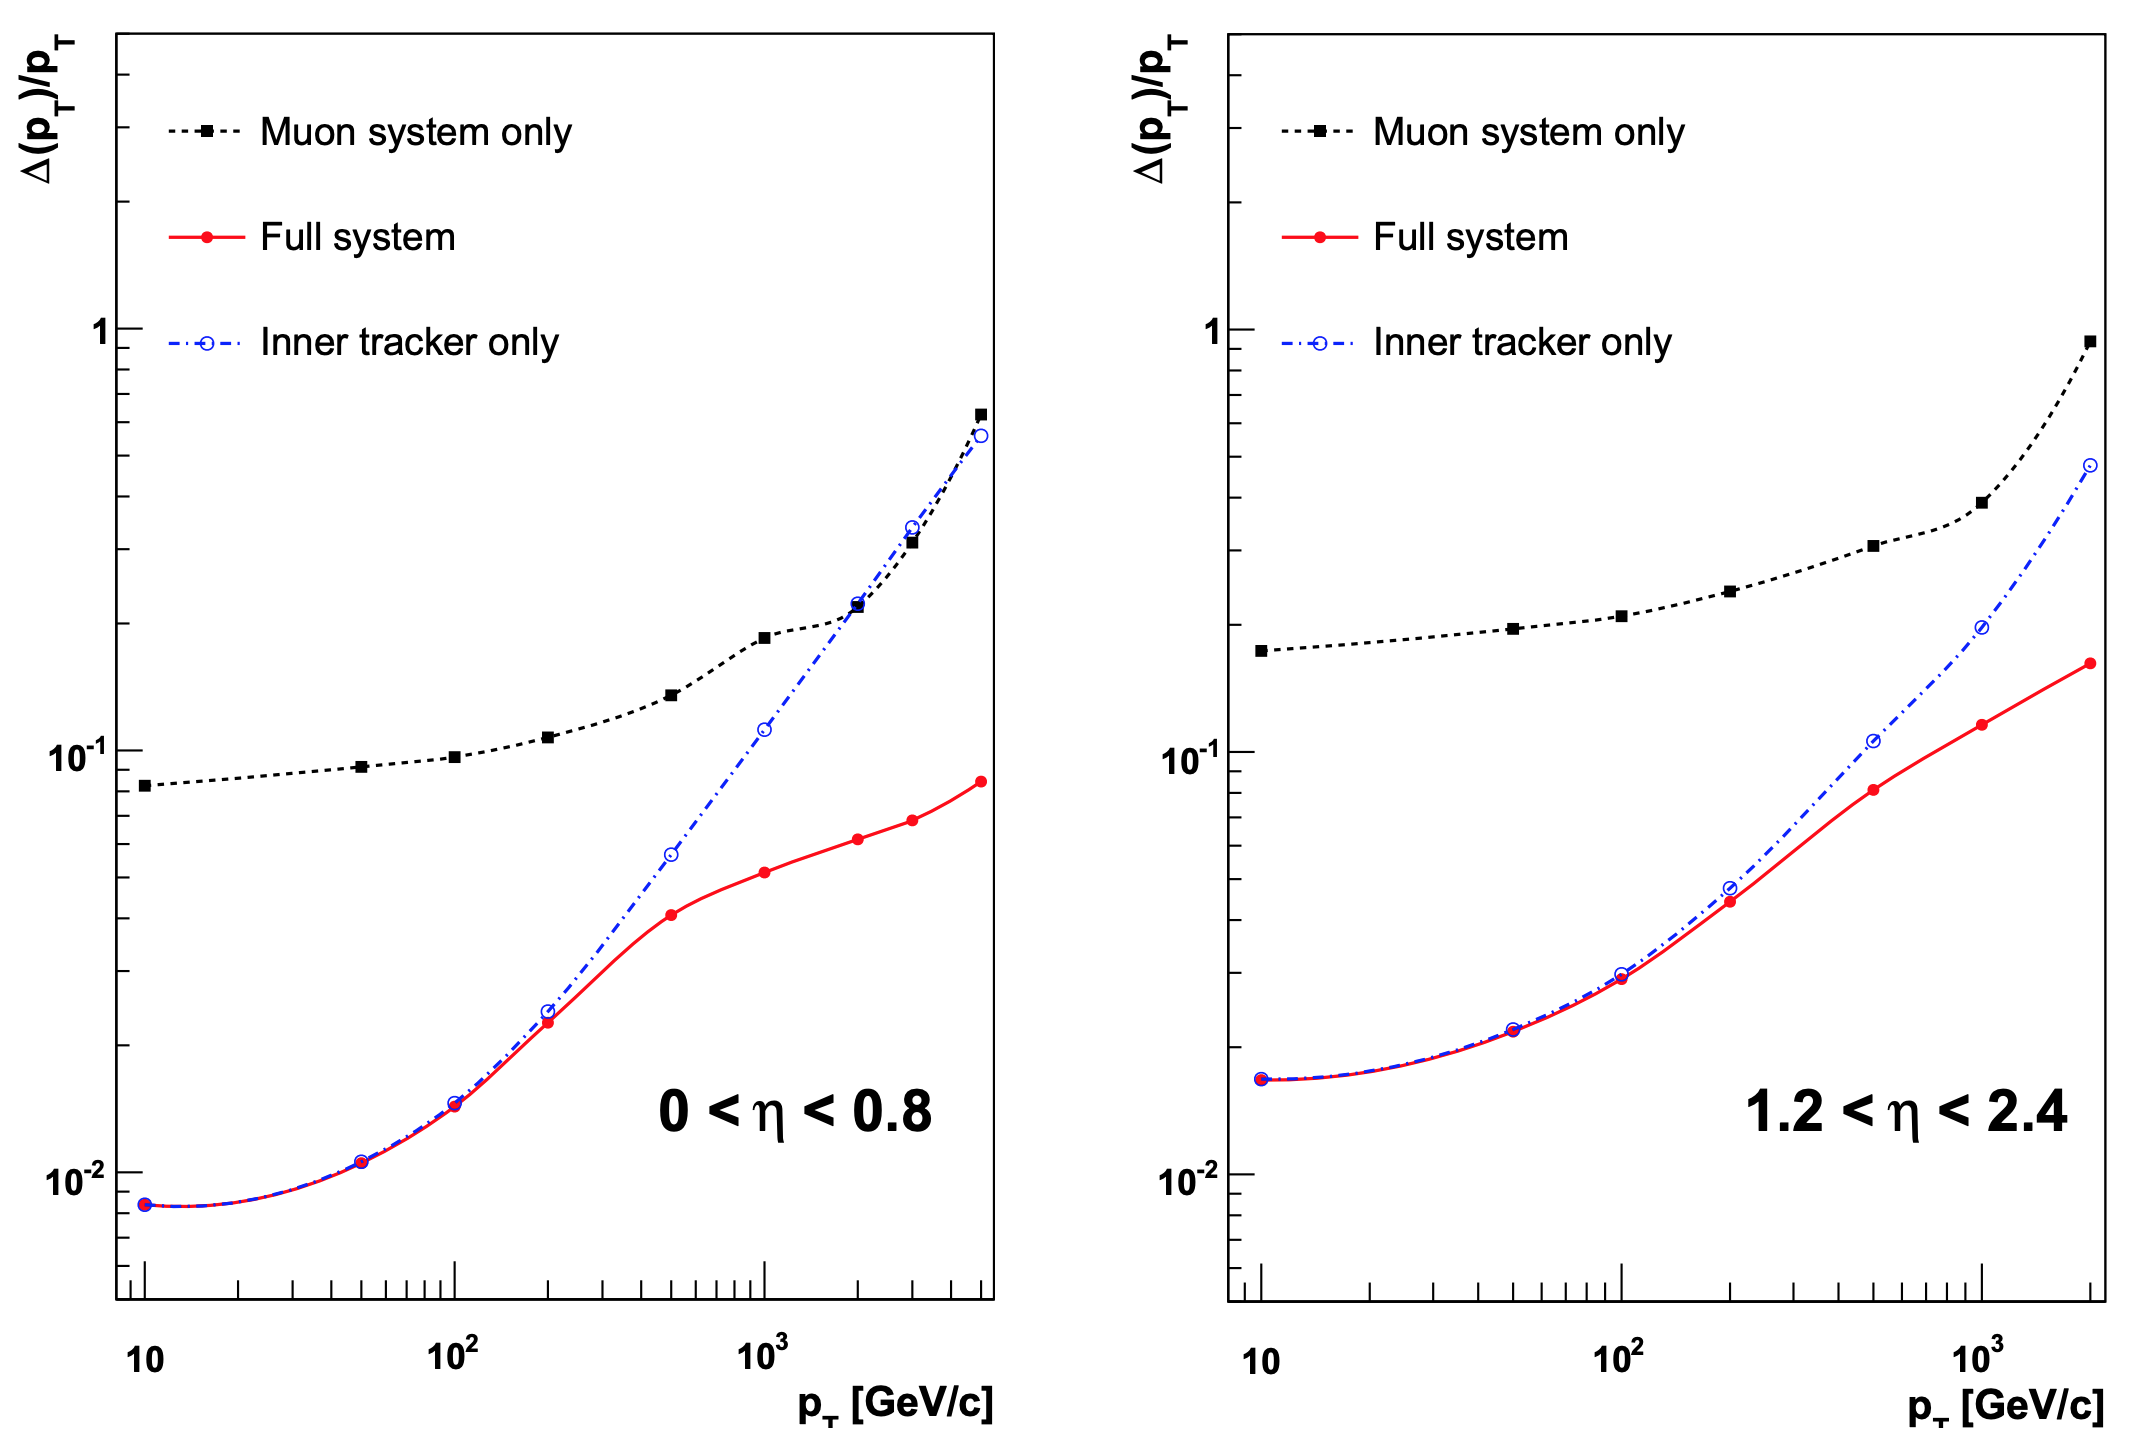
\includegraphics[width=0.8\linewidth]{figures/cms/cms_tracker_vs_muon.png}
    \caption{Fractional momentum resolution for muons reconstructed by the CMS detector, shown for reconstructions using the inner tracker only (blue), the muon system only (black), and the combination of measurements from both subdetectors (red). The muon system improves significantly the momentum resolution of $\mathcal O$(TeV) muons. Taken from~\cite{Chatrchyan:2008aa}.}
    \label{fig:cms_muon_vs_tracker}
\end{figure}

\subsection{Trigger System} \label{sec:cms_trigger}
At the LHC's design luminosity of $10^{34}$~cm$^{-2}$~s$^{-1}$, the pp interaction rate is greater than 1~GHz~\cite{Khachatryan:2016bia}.
It is neither necessary nor feasible to store the data of each of the more than $10^9$ events per second, as the vast majority of pp interactions are neither interesting nor useful in light of the goals of the CMS physics program.
It is not feasible in the sense that the CMS readout electronics impose an upper limit on the event rate of about 100~kHz, such that the vast majority of events must be thrown away.
Is is not necessary in the sense that most physics processes of interest have cross sections many orders of magnitude smaller than the nominal pp interaction cross section.

In order to select only the most interesting events to store for later analysis, a two-tiered trigger system is employed by the CMS detector.
The first level (L1), is implemented on custom hardware, and reduces the event rate by a factor of about $10^4$, from around 1~GHz to around 100~kHz.
The second level (HLT), is implemented in software, and further reduces the event rate to a typical rate of 400~Hz.

\subsubsection{L1 Trigger}
The L1 trigger combines information from the ECAL, HCAL, and muon system to decide with a fixed latency of 4~$\mu$s of a collision if the event should be accepted or not.
A schematic overview of the trigger system is shown in Fig.~\ref{fig:cms_l1_trigger}.
Events which pass the L1 trigger are then evaluated by the high-level trigger system to make a final decision on if the full event data will be stored.

\begin{figure} [htbp!]
    \centering
    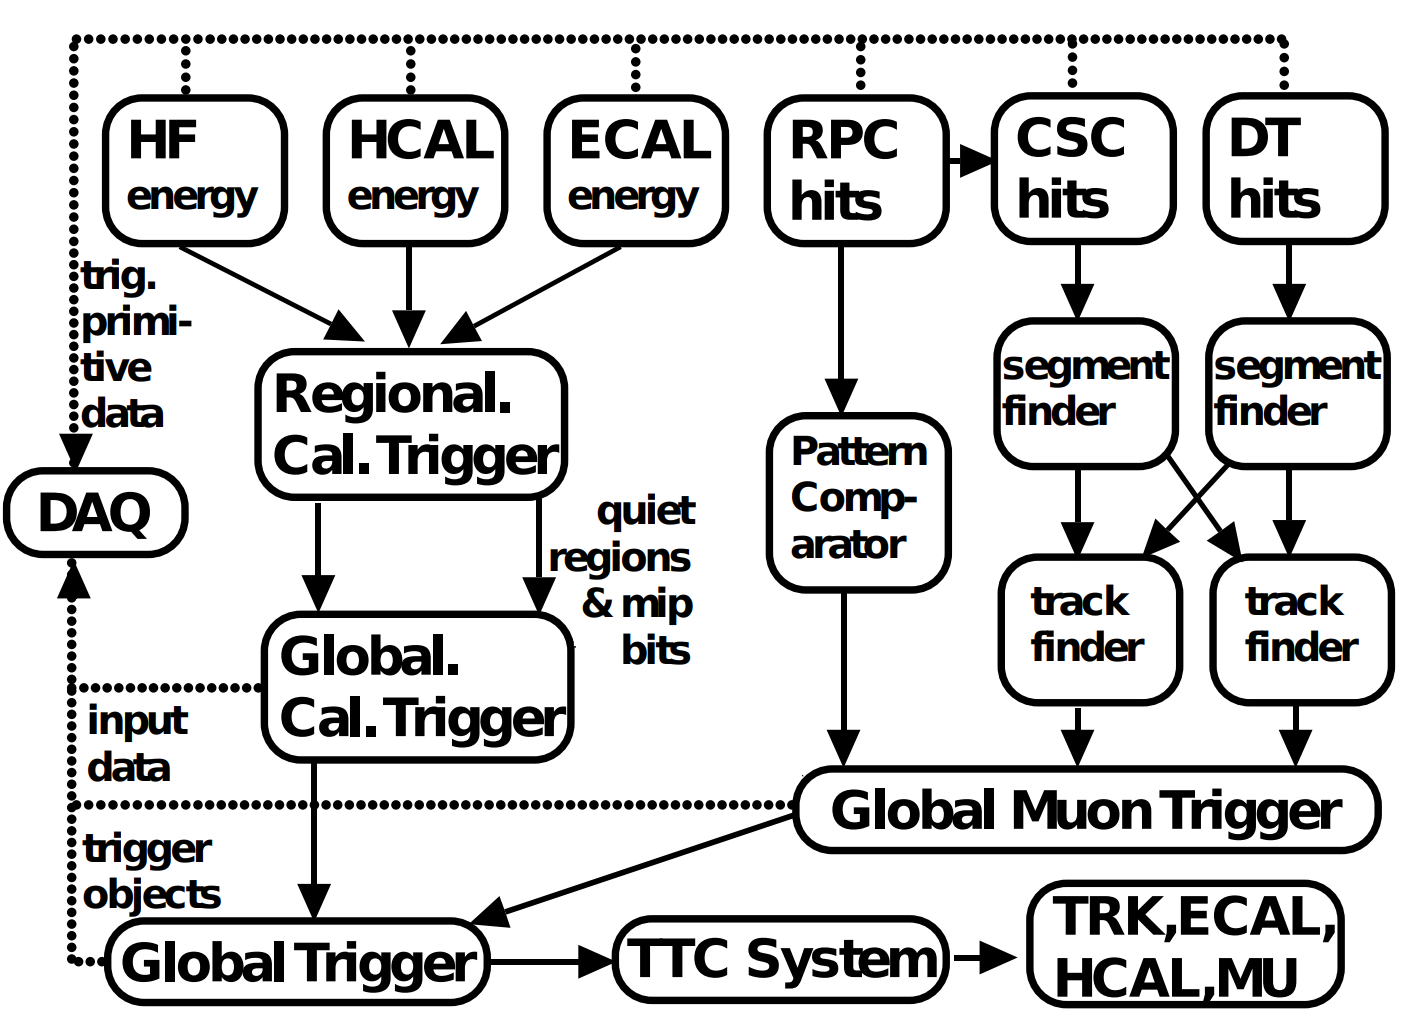
\includegraphics[width=0.6\linewidth]{figures/cms/cms_l1_trigger.png}
    \caption[Schematic overview of the CMS L1 trigger system. Taken from~\cite{Khachatryan:2016bia}.]{Schematic overview of the CMS L1 trigger system. Information from the calorimeters are first processed regionally and then a global calorimeter decision (GCT) is made. Similarly, information from the various components of the muon system are first processed regionally and then at a global level (GMT). The information from the global calorimeter trigger and global muon trigger are combined in a single global trigger (GT) which performs the final decision on whether to store the event. Taken from~\cite{Khachatryan:2016bia}.}
    \label{fig:cms_l1_trigger}
\end{figure}

\subsubsection{High-Level Trigger}
In contrast to the L1 trigger, the high-level trigger (HLT) system accepts events for storage based off a more complete, nearly offline-quality reconstruction of the event.
Details of event reconstruction, e.g. the particle flow algorithm, are describe in Sec.~\ref{sec:evt_pf}.
Near offline-quality event reconstruction is achieved in practice through the use of a ``processor farm'', a system of over $10^4$ CPUs working in parallel to efficiently reconstruct each event.
The HLT takes significantly longer to ``think'' about each event, with an average processing time on the order of 100~ms per event (compare to 4~$\mu$s for L1).

The high-level trigger paths used for the \ttH (\Hgg) analysis are the following:
\begin{itemize}
    \item 2016: \texttt{HLT\_Diphoton30\_18\_R9Id\_OR\_IsoCaloId\_AND\_HE\_R9Id\_Mass90*}
    \item 2017: \texttt{HLT\_Diphoton30\_22\_R9Id\_OR\_IsoCaloId\_AND\_HE\_R9Id\_Mass90*}
    \item 2018: \texttt{HLT\_Diphoton30\_22\_R9Id\_OR\_IsoCaloId\_AND\_HE\_R9Id\_Mass90*}
\end{itemize}

Conceptually, each of these triggers requires the presence of two photons with leading (subleading) transverse momenta of 30 (18/22) GeV, imposes requirements on the photons' shower shape variables (described in further detail in Sec.~\ref{sec:evt_photon}), and requires a diphoton invariant mass of at least 90 GeV.
The photon selection requirements described in Sec.~\ref{sec:evt_photon} are defined to be similar (and slightly stricter) than those of the trigger paths listed here.
Still, the efficiency of the trigger in simulation does not necessarily match that in data.
The efficiency is measured in data with \Zee events and the efficiency in simulation is accordingly corrected as a function of the transverse energy, pseudorapditity, and shower shape variable $R_9$ (defined in Sec.~\ref{sec:evt_photon}), with the uncertainty on the scale factor taken as a systematic uncertainty (described in Sec.~\ref{sec:tth_systematic_uncertainties}). 


\chapter{Event Reconstruction and Selection}

\section{Introduction} \label{sec:evt_intro}
The raw data recorded by the CMS detector for a single bunch crossing is typically not yet suitable for high-level physics analysis.
Several layers of abstraction transform the data from the raw detector readout into high-level physics objects.
The first layer of abstraction uses the particle flow (PF) algorithm \cite{particle_flow}, which combines information from each of the CMS subdetectors (the tracker, ECAL, HCAL, and muon system) in an attempt to reconstruct every particle in the event (PF candidates).
Physics objects are then refined further by placing quality requirements on the PF candidates.


\section{The Particle Flow Algorithm} \label{sec:evt_pf}
The PF algorithm forms the basis of event reconstruction for almost all physics analyses in CMS.
It attempts to individually reconstruct every particle in a given event, doing so by combining information from each of the CMS subdetectors.
The fundamental inputs to the PF algorithm are tracks, originating from the tracker and muon system, and calorimeter clusters, obtained from the ECAL and HCAL.
Combining each of these pieces of information results in more accurate reconstruction of individual particles (and by extension, hadronic jets).
Notably, jets built from PF candidates contain 95--97\% of the jet energy, compared 60--80\% for jets built solely from calorimeter clusters.
The angular resolution of jets is also improved by a factor of 2--3~\cite{beaudette2014:Brient:2013hsa}.

Tracks are reconstructed in three stages using a procedure based on Kalman-Filtering.
First, seeds are generated using a small number of hits compatible with a track.
Second, compatible hits in other tracker layers along the trajectory of this track are identified.
Finally, a fit is performed with each of the hits in order to determine the properties associated with the candidate particle: origin, transverse momentum, and direction.
In order to prevent the identification of fictitious tracks, a set of strict quality criteria are imposed upon the candidate tracks.
Tracks are required to have a minimum amount of transverse energy ($\pT > 0.9$ GeV), must be seeded from hits in at least two consecutive layers in the pixel detector, must have at least 8 total hits, and may be missing hits in at most 1 layer.
While these requirements allow the tracking algorithm to maintain a low misidentification rate, they also exclude around 20-30\% of charged hadron tracks with $\pT > 1$ GeV.
Charged hadron tracks frequently do not pass the track requirements because of their high probability to undergo nuclear interactions with the beam pipe or detector material before reaching the outer tracker.
Muons with $\pT > 1$ GeV, on the other hand, have a negligible probability of interacting before reaching the outer tracker and consequently have a much higher tracking efficiency of 99\%.

Clusters in the ECAL and HCAL are built by first identifying a seed, a cell with energy larger than a certain seed threshold and also larger than the energy of neighboring cells.
The ECAL and HCAL cells are of a size such that a typical particle interacting with either calorimeter will leave its energy distributed across multiple neighboring cells.
If two particles enter a calorimeter close to each other, some cells may receive energy contributions from both particles.
To address scenarios like this, topological clusters are formed by joining cells that are ``once-removed'' from the seed (i.e. they share at least one neighbor with a seed) with an energy larger than a certain threshold, not necessarily the same as the seed threshold.
The energy of each cluster within a topological cluster is then determined by a maximum-likelihood fit to a sum of Gaussians.
The number of Gaussians is the number of seeds in the topological cluster and the parameters to fit are the energy of each cluster (the amplitude of each Gaussian), $A_i$, and the position ($\eta_i, \phi_i$) of each cluster.
The initial values for the energy and position of each cluster are chosen as the energy and position of the corresponding seed.
The width for each Gaussian is fixed and depends on the specific calorimeter.

A link algorithm then combines compatible tracks and clusters, using the full set of information to reconstruct five different types of particles:
\begin{itemize}
    \item \textbf{Muons:} reconstruction based on tracks from both the inner tracker and the muon system.
    \item \textbf{Electrons:} tracks for electrons are reconstructed with a Gaussian-sum filter (GSF) that allows for sudden loss of energy due to bremsstrahlung. GSF tracks linked to an ECAL supercluster are then chosen as electron candidates.
    \item \textbf{Photons:} reconstruction based on ECAL superclusters which are \emph{not} linked to GSF tracks.
    \item \textbf{Charged hadrons:} reconstruction based on tracks that are linked to both ECAL and HCAL clusters.
    \item \textbf{Neutral hadrons:} reconstruction based on HCAL clusters which are \emph{not} linked to tracks or ECAL superclusters.
\end{itemize}

The PF algorithm does not attempt to distinguish between different types of charged or neutral hadrons.


\section{Vertex Reconstruction} \label{sec:evt_vertex}
For data collected by the CMS detector during Run II of the LHC, the mean number of of primary interactions was $\mu = 29$. 
The primary vertex is taken to be the one with the largest value of the sum of the squares of the transverse momenta of the physics objects~\cite{Contardo:2020886}.
In other words, it is chosen as:
\begin{equation}
    \argmax_{i \in \mathcal I} f(i), \qquad f(i) \equiv \sum_{j=1}^{N_i} (\pT^j)^2
\end{equation}
where the sum runs over the $N_i$ physics objects associated with the $i$-th vertex.

For many \Hgg analyses, this prescription of choosing the primary vertex is suboptimal, as it relies on charged tracks linked to the primary vertex and as photons are neutral particles, they do not leave tracks.
However, for the \ttH analysis in which additional jets and leptons are expected in the final state, this choice of primary vertex is found to be the correct choice for $>99$\% of \ttH events, so no further vertex selection criteria are employed. % FIXME cite 2017 ttH AN for vertex efficiency?


\section{Photon Reconstruction} \label{sec:evt_photon}
The photons selected for use in this analysis are initially taken from the PF photon candidates described in Sec.~\ref{sec:evt_pf}.
In further reconstruction of photons for \Hgg analyses, there are several challenges to overcome.

First, the energy estimate provided by the PF algorithm generally has inherent bias.
The bias in the photon energy estimates are corrected for with a regression technique which utilizes \Zee events in which the electrons have been reconstructed as photons.
The procedure, described in Sec.~\ref{sec:evt_photon_energy} exploits the fact that the mass of the Z boson is known~\cite{Tanabashi:2018oca} to good precision, ensuring that the \mee distribution is centered around \mZ.
An additional smearing procedure corrects for the differences in energy resolution between data and simulation.
This step is vital as simulation, rather than actual data, is used to construct the models of SM Higgs boson production modes, including \ttH.

A second challenge in \Hgg analyses is distinguishing between ``prompt'' photons and ``fake'' photons.
Prompt photons are those produced in the decay of the Higgs boson or from the primary hard inelastic scattering process and are typically the objects of interest of physics analyses.
Fake photons are those produced in hadronic jets, usually through the decay \Pigg, and are (typically) of less interest.
Prompt photons tend to be more isolated in the detector and tend to have different shower shapes in the ECAL.
These differences are exploited through the used of a BDT trained to distinguish between prompt and fake photons.

The photon ID BDT, described in Sec.~\ref{sec:evt_photon_idmva}, uses a variety of high-level variables describing the photon's kinematics, shower shape, and isolation.
The shower shape \& isolation variables and the photon ID BDT are used to select photons of interest for the \ttH analysis, rejecting as many fake photons as possible while retaining a high efficiency on prompt photons.
As simulation is used to construct the models of SM Higgs boson production modes, it is important that the shower shape \& isolation variables and the photon ID BDT are well-described in simulation.
A chained quantile regression method, described in Sec.~\ref{sec:evt_photon_ss}, corrects the distributions of these features in simulation.
The multitude of high-level variables used to describe photons are defined in Sec~\ref{sec:evt_photon_vardef}.
 
\subsection{Variable Definitions} \label{sec:evt_photon_vardef}
The variables defined in this section are used for studying the scale \& resolution of photon energy reconstruction, discriminating between prompt and fake photons, selecting the photons to be used in analysis, or a combination of the three.

\subsubsection*{General}
\begin{itemize}
    \item \emph{Conversion-safe electron veto}: a flag rejecting the photon candidate if there is a track with at least one hit in the inner layer of the pixel detector pointing to the photon supercluster \emph{and} the track is not matched to a vertex. 
    \item \emph{Pixel seed veto}: a flag rejecting the photon candidate if any track with at least two hits points to the photon supercluster. In general, the pixel seed veto provides a more severe rejection of electrons but excludes a larger fraction of photons.
    \item $\rho$: the median energy density per unit area in the event. 
\end{itemize}

The pixel seed veto is, in general, much stricter than the conversion-safe electron veto in rejecting electrons imitating photons.
For most \Hgg analyses, electrons are not a large source of fake photons and so the conversion-safe electron veto is used for its greater efficiency on real photons.
However, the \ttH analysis has a significant background component coming from \ttplusX events in which an electron from a $\PW \to \Pe\nu_{\Pe}$ decay is reconstructed as a photon.
To target this background, the pixel seed veto is employed (as a training variable in the BDT used to define signal regions).

\subsubsection*{Shower shape variables}
\begin{itemize}
    \item $E_{2\times2}/E_{5\times5}$: the ratio of energies between $2\times2$ and $5\times5$ matrices of ECAL crystals. The $2\times2$ matrix is defined as that containing the two most energetic crystals, the $5\times5$ matrix is defined as that centered on the supercluster seed crystal.
    \item \emph{cov}$_{i\eta i\phi}$: the covariance of the crystal values of the $5\times5$ matrix centered on the supercluster seed crystal.
    \item $\sigma_{i\eta i\eta}$: the standard deviation along the $\eta$ direction of the electromagnetic shower (expressed in terms of crystal cells).
    \item $R_9$: $E_{3\times3}/E_{\text{SC}}$, where $E_{3\times3}$ is the $3\times3$ crystal matrix centered on the supercluster seed crystal and $E_{\text{SC}}$ is the total energy of the supercluster.
    \item $\sigma_\eta$: the standard deviation of crystal $\eta$ values in the supercluster, with each crystal's contribution weighted by the logarithm of its energy.
    \item $\sigma_\phi$: the standard deviation of crystal $\phi$ values in the supercluster, with each crystal's contribution weighted by the logarithm of its energy.
    \item \emph{Preshower} $\sigma_{RR}$: the standard deviation of the shower spread in the $x$ and $y$ directions of the preshower detector (defined only in the endcap).
\end{itemize}

The shower shape variables are useful in both the regression of photon energy and the discrimination between prompt photons and hadronic jets misidentified as photons (``fake'' photons).

\subsubsection*{Isolation variables}
\begin{itemize}
    \item $\mathcal I_{\text{ph}}$: the transverse energy sum of all other PF photons in a cone size $R=0.3$ around the photon candidate.
    \item $\mathcal I_{\text{ch, sel}}$: the transverse energy sum of all PF charged hadrons in a cone size $R=0.3$ around the photon candidate, measured with respect to the selected vertex.
    \item $\mathcal I_{\text{ch, wst}}$: the transverse energy sum of all PF charged hadrons in a cone size $R=0.3$ around the photon candidate, measured with respect to the worst-fit vertex.
    \item $H/E$: the energy sum from the HCAL towers within a cone of $R=0.15$ around the supercluster, divided by the energy of the supercluster.
    \item $\mathcal I_{\text{tk}}$: the transverse momentum sum of all tracks in a cone size $R=0.3$ around the photon candidate. Tracks within an inner cone size $R=0.04$ are \emph{not} included in this sum, effectively making the sum over a ``hollow'' cone.
\end{itemize}

The isolation variables are useful in discriminating between prompt photons and hadronic jets misidentified as photons.

\subsection{Energy Scale \& Resolution Corrections} \label{sec:evt_photon_energy}
The energy measurements of individual ECAL channels are first corrected, as described in Sec.~\ref{sec:cms_ecal}.
Once the ECAL energy measurements are calibrated, a multivariate regression technique~\cite{Khachatryan:2015iwa} is used to further correct the energy of photon candidates.
After the multivariate regression is applied, further energy scaling is applied to correct for any time or position dependent bias effects in the energy measurements in data.
Lastly, a smearing procedure is applied to simulation such that the energy resolution from simulation matches that in data.

The multivariate regression attempts to correct for many systematic sources of bias in the supercluster energy measurement.
For example, the supercluster may not capture all of the electromagnetic shower from a given photon (thereby underestimating its energy).
These sources typically relate to the details of the ECAL geometry (i.e. the geometrical arrangement of crystals and voids between crystals) and the probability of interaction with detector material before reaching the ECAL.
Among the training inputs for the regressor are the supercluster coordinates ($\eta$ and $\phi$), shower shape variables, information about the seed crystal of the supercluster, and variables ($\rho$ and number of vertices) describing the pileup conditions of the event. 

The regressor attempts to predict the form of the probability distribution function for $E_{\text{true}}/E_{\text{raw}}$.
The functional form for the probability distribution function for $E_{\text{true}}/E_{\text{raw}}$ is chosen as a Gaussian with two power law tails.
The regressor simultaneously predicts the true energy and the uncertainty in the energy measurement for a given photon, by returning values of the parameters for the functional form.
The true energy, $E_{\text{true}}$ is taken as the most probable value of the probability distribution function returned by the regressor.
The energy resolution is determined from the width of the probability distribution function. 
The sum of probability distribution functions returned by the regressor are compared to the actual $E_{\text{true}}/E_{\text{raw}}$ distribution (in simulation) in Fig.~\ref{fig:photon_energy_regression}.
\begin{figure} [h!]
    \centering 
    \begin{tabular}{c c}
        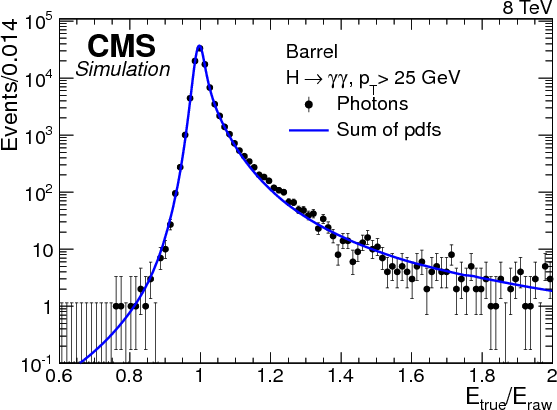
\includegraphics[width=0.48\linewidth]{figures/event_reconstruction_and_selection/figs_recoenergy_Fig-2a.png} &
        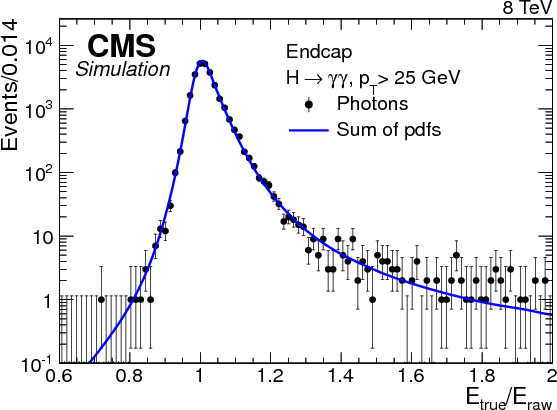
\includegraphics[width=0.48\linewidth]{figures/event_reconstruction_and_selection/figs_recoenergy_Fig-2b.png}
    \end{tabular}
    \caption{Sum of probability distribution functions returned by the regressor (blue) compared with the actual $E_{\text{true}}/E_{\text{raw}}$ distribution in simulation (black). Taken from~\cite{Khachatryan:2015iwa}}.
    \label{fig:photon_energy_regression}
\end{figure}

Next, an energy scaling procedure is applied on data to correct any non-uniformity in time or position ($\eta$) in the energy measurements.
Sources of bias include damage to the ECAL due to radiation, for example.
Since the detector response changes as a function of $\eta$ (radiation damage is not uniform in $\eta$) and as a function of time (damage is ``cumulative''), the scale correction is derived in bins of $\eta$ and run number.
This procedure exploits the known mass of the Z boson by using an analytic fit to the invariant mass of electrons reconstructed as photons in \Zee events in data and simulation.
The functional form in the fit is the convolution of a Breit-Wigner~\cite{Breit:1936zzb} and a Crystal Ball function, with the Crystal Ball modeling both the calorimeter resolution effects and losses due to bremsstrahlung.
The parameters of the Breit-Wigner are fixed to the Particle Data Group values~\cite{Tanabashi:2018oca} of \mZ and $\Gamma_{\PZ}$.
The scale correction is calculated from the difference in the mass peaks between data and simulation:
\begin{equation}
    \Delta P = \frac{m_{\text{data}} - m_{\text{MC}}}{\mZ}
\end{equation}
While the Z mass peak initially varies by a few percent as a function of $\eta$ and run number, the peak is stable after applying the scale corrections to data. %, as Fig.~\ref{fig:photon_scales} shows.

%Moreover, the reconstructed Z peak is quite consistent between data and simulation.
%\begin{figure} [h!]
%    \centering
%    \begin{tabular}{c c}
%        \includegraphics[width=0.48\linewidth]{figures/event_reconstruction_and_selection/hig19015_Figure_002-a.pdf} &
%        \includegraphics[width=0.48\linewidth]{figures/event_reconstruction_and_selection/hig19015_Figure_002-b.pdf}
%    \end{tabular} 
%    \caption{Taken from \cite{CMS:2020omd}.}
%    \label{fig:photon_scales}
%\end{figure}
Finally, a smearing procedure is applied to the energy measurements in simulation to ensure that the energy resolution in simulation matches that observed in data.
The additional smearing applied to simulation is a Gaussian function and its properties are determined by a fit to the Z invariant mass peak.
The smearings are derived with the same bins as the energy scales.

The regression, scales, \& smearings are validated by comparing the invariant mass distribution of electrons reconstructed as photons in \Zee events between data and simulation.
Fig.~\ref{fig:photon_energy_validation} shows that excellent agreement between data and simulation is achieved for all three years of data-taking.
\begin{figure} [h!]
    \centering
    \begin{tabular}{c c}
        \includegraphics[width=0.48\linewidth]{figures/event_reconstruction_and_selection/hig19015_Figure_002-a.pdf} &
        \includegraphics[width=0.48\linewidth]{figures/event_reconstruction_and_selection/hig19015_Figure_002-b.pdf}
    \end{tabular}
    \caption{Validation of photon energy regression, scales, and smearings: comparisons of $m_{ee}$ distributions in \Zee events. Taken from \cite{CMS:2020omd}.}
    \label{fig:photon_energy_validation}
\end{figure}
An additional, ``residual'', scale correction is derived simultaneously with the smearings.
The residual scale correction, applied on top of the run-dependent scale corrections previously described, corrects for any remaining differences between the central value of \PZ mass peak in data and simulation (which match by construction of the run-dependent scale corrections) and the central value of the \PZ mass peak known from the well-measured mass of the \PZ.
The run-dependent scale corrections ensure agreement between data and simulation, while the residual scale corrections ensure agreement between data, simulation and the known mass of the \PZ.
Each of the run-dependent scale corrections, residual scale corrections, and smearing corrections range from approximately 1--3\%.

\subsection{Shower Shape \& Isolation Corrections} \label{sec:evt_photon_ss}
The shower shape and isolation variables that are used in training the photon ID BDT show disagreement between data and simulation.
Because of the disagreement in the input variables, disagreement between data and simulation in the photon ID BDT score is also observed.
The distributions of these variables in simulation are corrected with a chained quantile regression method~\cite{DBLP:journals/corr/abs-1211-6581}.
Each variable is corrected using separately trained BDTs, each trained to predict the conditional shape of the cumulative distribution function in both data and simulation.
The value in simulation is replaced by the value corresponding to the same point on the cumulative distribution function in data.
The BDTs take the photon kinematics, $\rho$, and the variables that have already been corrected as inputs.
The variables that have already been corrected are given as additional inputs in order to better preserve the correlations between the input variables in data.
After applying this method, good agreement between data and simulation in the photon ID BDT output is achieved for all three years, as seen in Fig.~\ref{fig:photon_idmva}.

\subsection{Photon Identification BDT} \label{sec:evt_photon_idmva}
A common challenge to all \Hgg analyses is the discrimination between prompt and fake photons.
\begin{itemize}
    \item \textbf{Prompt photons:} photons which are external lines in the Feynman diagram of the primary hard inelastic scattering process of the event.
    \item \textbf{Fake photons:} all other photons. Primarily composed of hadronic jets in which a \Pigg decay results in the jet being misidentified as a photon.
\end{itemize}
Broadly speaking, distinguishing between the two is an easy problem.
Prompt photons tend to be \emph{isolated} in the detector, meaning there are few particles in close physical proximity.
Fake photons tend not to be isolated, as they are overwhelmingly hadronic jets and therefore typically accompanied by a shower of hadronic activity.
However, the characteristic scale for the cross sections of multi-jet production is many orders of magnitude larger than the characteristic scale for the cross sections of Higgs boson production.
While the vast majority of hadronic jets can easily be distinguished from prompt photons, the ``tails of the distribution'', in which the electromagnetic activity of a hadronic jet may be quite isolated, provide a challenging background.

A binary classifier BDT is trained to distinguish between the two cases, helping further reduce the contribution of fake photons to the background.
The BDT is trained on simulation of \gjets events.
Signal events are prompt photons, taken as reconstructed photons which are matched to a generator-level photon from the hard inelastic scattering process
The matching procedure is done by requiring a maximum $\Delta R$ between the reconstructed and generator-level photons.
Background events are taken as all other reconstructed photons in the event.
These are overwhelmingly populated by hadronic jets misidentified as photons.
The BDT is trained with the (previously defined) shower shape and isolation variables.
The photon ID BDT is validated with two methods, both exploiting the tag-and-probe method.
The first uses \Zee events in which electrons are reconstructed as photons and the second uses \Zuug events in which the \PZ decays to two muons and one of the muons radiates a photon.
Good agreement between data and simulation is found with both methods. Fig.~\ref{fig:photon_idmva} shows the agreement in \Zee events.
\begin{figure} [h!]
    \centering
    \includegraphics[width=0.7\linewidth]{figures/event_reconstruction_and_selection/hig19015_Figure_003-b.pdf}
    \caption{Validation of the photon ID BDT in \Zee events: comparison of distributions in data and simulation. Taken from \cite{CMS:2020omd}.}
    \label{fig:photon_idmva}
\end{figure}

\subsection{Selection Criteria} \label{sec:evt_photon_sel}
As described in Sec.~\ref{sec:cms_trigger}, the data-taking rate imposes a formidable challenge on identifying events of interest.
Events in data will only enter the analysis provided they pass one of the HLTdiphoton triggers used for this analysis (described in Sec.~\ref{sec:cms_trigger}).
The trigger is not applied on simulation, so the preselection requirements are chosen to be slightly more stringent than those of the trigger: events (in data or simulation) passing the preselection requirements are a subset of events passing the HLT trigger.

The photon with the highest transverse momentum (``leading'') is required to have $\pT > 35$ GeV, and the photon with the second highest transverse momentum (``subleading'') is required to have $\pT > 25$ GeV.
To ensure that the \mgg distribution has a smooth shape, ``sliding'' \pT requirements of $\pT/\mgg > 1/3 (1/4)$ are imposed for the leading (subleading) photon.
Without the sliding \pT requirements, the \mgg distribution may be subject to features like peaks at lower \mgg: since individual photon \pT is positively correlated with \mgg, fixed \pT requirements reject a greater fraction of low \mgg events.
It is preferable to avoid these features to ensure that the \mgg distribution may be fit by simple analytic functions (the background estimation method, described later, relies on this assumption).

Photons must have $R_9 > 0.8$, $\mathcal I_{\text{ch, sel}} < 20$ GeV.
If a photon has $\pT > 14$ GeV and $H/E < 0.15$, it must also satisfy $\mathcal I_{\text{ch, sel}}/\pT < 0.3$.
Additional requirements on the isolation variables are imposed as a function of the photon location (barrel vs. endcap) and $R_9$, summarized in Table~\ref{tab:photon_presel}.
\begin{table} [h!]
    \centering
    \begin{tabular}{ l r | l | l | l | l } \hline \hline
        & & $H/E$ & $\sigma_{i\eta i\eta}$ & $\mathcal I_{\text{ph}}$ & $\mathcal I_{\text{tk}}$  \\ \hline
        \multirow{2}{*}{Barrel} & $0.5 < R_9 < 0.85$ & $<0.08$ & $<0.015$ & $<4.0$ GeV & $<6.0$ GeV \\
                                & $R_9 \geq 0.85$ & $<0.08$ & -- & -- & -- \\ \hline
        \multirow{2}{*}{Endcap} & $0.5 < R_9 < 0.9$ & $<0.08$ & $<0.035$ & $<4.0$ GeV & $<6.0$ GeV \\
                                & $R_9 \geq 0.9$ & $<0.08$ & -- & -- & -- \\ \hline \hline 
    \end{tabular}
    \caption{Photon preselection requirements. Values are chosen to be slightly more stringent than the HLT requirements.}
    \label{tab:photon_presel}
\end{table}


\section{Jet Reconstruction} \label{sec:evt_jet}
As discussed in Sec.~\ref{sec:pp_physics_jets}, color confinement prevents the existence of free quarks and gluons.
A quark or gluon produced at the LHC typically undergoes hadronization and presents itself in the detector as a collection of collimated particles.
Jets are built from PF candidates, using the anti-$k_{\text{T}}$ clustering algorithm~\cite{Cacciari:2008gp,Cacciari:2011ma} with a distance parameter of 0.4.
The input PF candidates have charged hadron subtraction (CHS) applied, meaning charged hadrons associated with vertices other than the primary vertex of that event are removed.
CHS reduces the contribution of particles originating from pileup vertices.
Once the jets are built from PF candidates, three steps are taken to correct the jets' energies.

First, a pileup offset correction is applied to remove additional jet contributions from pileup not removed by CHS.
The pileup contributions not remove by CHS are primarily charged hadrons not matched to a good vertex and PF photons.
The individual jet energies are corrected by a multiplicative factor derived in simulation, parametrized in bins of jet area ($A$), $\rho, \pT,$ and $\eta$.
Typical values for the pileup offset corrections are shown in Fig.~\ref{fig:evt_jet_pu_corrections}.
\begin{figure} [h!]
    \centering
    \begin{tabular}{c c}
        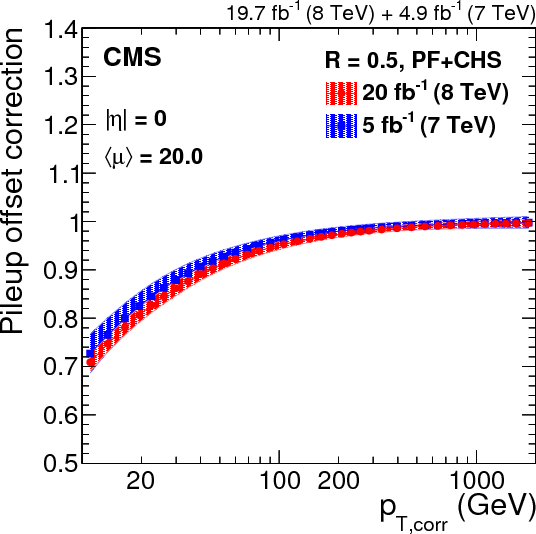
\includegraphics[width=0.48\linewidth]{figures/event_reconstruction_and_selection/jetmet8Tev_Figure_009-c.png} &
        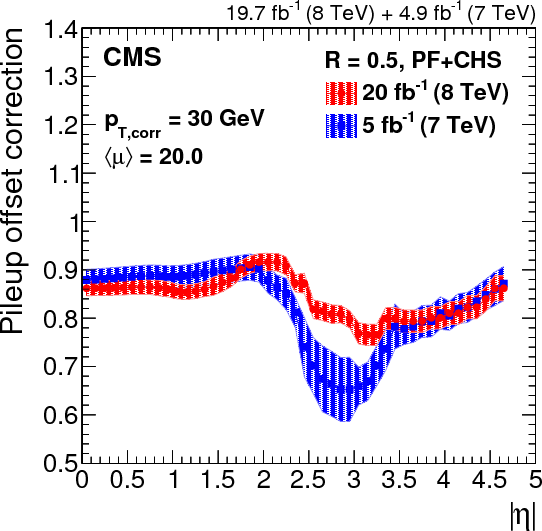
\includegraphics[width=0.48\linewidth]{figures/event_reconstruction_and_selection/jetmet8Tev_Figure_009-d.png}
    \end{tabular}
    \caption{Pileup offset correction values as a function of jet \pT (left) and jet $|\eta|$ (right). Taken from~\cite{Khachatryan_2017_jets}}
    \label{fig:evt_jet_pu_corrections}
\end{figure}

Second, jet energy scale corrections designed to correct for the detector response to jets are derived in simulation, again in bins of jet area ($A$), $\rho, \pT,$ and $\eta$.
The goal of this step is to correct the reconstructed jet energy to match that of the true jet energy (only available in simulation).
Typical values for the jet energy scale corrections are shown in Fig.~\ref{fig:evt_jet_jec_corrections}. 
\begin{figure} [h!]
    \centering
    \begin{tabular}{c c}
        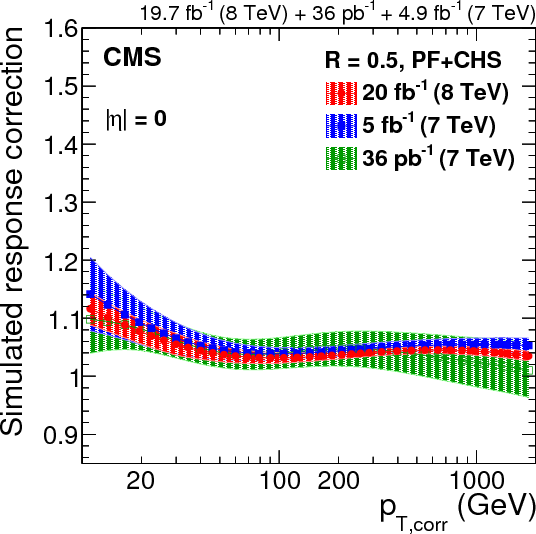
\includegraphics[width=0.48\linewidth]{figures/event_reconstruction_and_selection/jetmet8Tev_Figure_014-a.png} &
        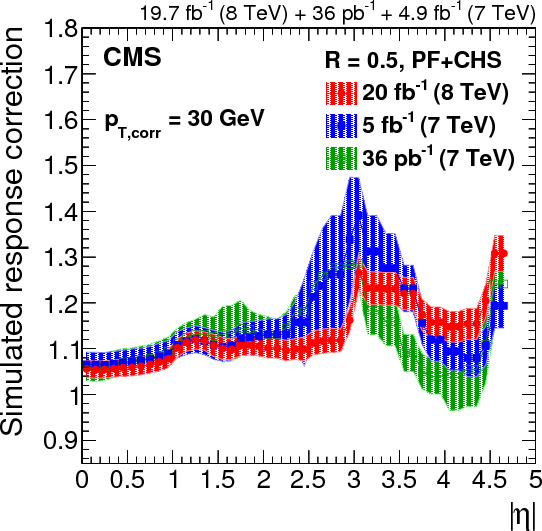
\includegraphics[width=0.48\linewidth]{figures/event_reconstruction_and_selection/jetmet8Tev_Figure_014-b.png}
    \end{tabular}
    \caption{Jet energy scale correction values as a function of jet \pT (left) and jet $|\eta|$ (right). Taken from~\cite{Khachatryan_2017_jets}}
    \label{fig:evt_jet_jec_corrections}
\end{figure}

Third, remaining differences between data and simulation are corrected with a residual correction applied to data, derived as a function of \pT and $\eta$.
A variety of event topologies ($\gamma$ + jets, \Zee + jets, \Zuu + jets, and di-jet) are used to derive these corrections.
In each topology, the underlying strategy is the same: exploit the momentum conservation in the transverse plane betwen a well-measured reference object and the jet to be corrected.
The fact that the reference object ($\gamma$, \Zee, \Zuu, a well-measured central jet) is well-measured allows us to infer the true energy of the jet to be corrected.
The full details of these procedures are described in Ref.~\cite{Khachatryan_2017_jets}.

Jets used in the \ttH analysis are first corrected with the procedures described in this section.
They are further required to have $\pT > 25$ GeV and $|\eta| < 2.4$ and must pass a loose pileup jet ID criteria.
The loose pileup jet ID criteria is based on a BDT designed to discriminate between jets originating from pileup interactions and those originating from the primary vertex in the event.
The BDT is trained with variables describing the jets' shape as well as additional track information.
Jets are finally also required to not be overlapping with any photons or leptons in the event, requiring $\Delta R(\text{jet}, \text{photon/lepton}) > 0.4$.

\subsubsection*{b-Tagged Jets}
Hadronic jets at the LHC typically result from the hadronization of either a quark or gluon (with the exception of top quarks, which decay before they are able to hadronize).
Jets originating from a light-flavor quark (u,d,s) or a gluon are typically indistinguishable in the CMS detector.
However, jets originating from c or b quarks often have distinguishing features. 
While hadrons containing only light-flavor quarks (as would typically be produced by the hadronization of a light-flavor quark or a gluon) often reach the calorimeters before decaying, hadrons containing b quarks tend to decay on a length scale of a few millimeters when produced at typical LHC energies.
Hadrons containing charm quarks frequently decay even sooner than this.
The resolution of the tracker is sufficient to distinguish the vertices of these decays, called ``secondary vertices'', from the primary vertices in the event.

Jet flavor tagging algorithms attempt to exploit information about the secondary vertices associated with a given jet to determine the flavor of the quark (or gluon) it originated from.
Machine learning algorithms are often used to classify jet flavor, using information about the secondary vertices, tracks, and pf candidates associated with a given jet.
Recently, algorithms built with deep neural networks have shown significantly improved jet flavor tagging performance over more traditionally used methods, such as those based on boosted decision trees~\cite{Guest_2016}.
The DeepCSV~\cite{Sirunyan_2018_deepcsv} algorithm is one such DNN-based tagger.
For a given jet, the algorithm assigns multiple flavor scores, indicating its degree of certainty that the jet originated from a quark of that flavor.
DeepCSV outputs scores corresponding to its degree of certainty that the jet originated from a b quark, c quark, light flavor quark (u,d,s) or gluon, and a \bb pair (four scores).
The performance of DeepCSV (purple) and other commonly used jet flavor algorithms is shown in Fig.~\ref{fig:evt_jet_btag}.
\begin{figure} [h!]
    \centering
    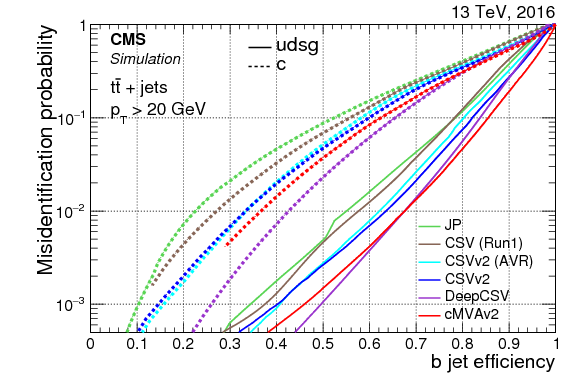
\includegraphics[width=\linewidth]{figures/event_reconstruction_and_selection/deepcsv_Figure_016.png}
    \caption{Misidentification rate as a function of b-tagging efficiency, shown for b vs. c jet discrimination (dotted lines) and b vs. light jet discrimination (solid lines). Taken from~\cite{Sirunyan_2018_deepcsv}.}
    \label{fig:evt_jet_btag}
\end{figure}

Jet flavor tagging is particularly useful for the \ttH analysis, as two b quarks are produced in the decay of the \ttb pair.
As the multi-jet, \gjets, and \dipho backgrounds primarily feature jets originating from light flavor quarks or gluons, the ability to select b-tagged jets allows for rejection of a significant component of the overall background.


\section{Lepton Reconstruction} \label{sec:evt_lepton}
Muons and electrons identified by the PF algorithm form the starting point for the leptons to be used in analysis.
\subsubsection*{Muons}
Muons are required to have $\pT > 5$ GeV and $|\eta| < 2.4$.
Next, a requirement is made on the mini-isolation of the muon, defined as
\begin{equation}
\mathcal I_{\text{mini}} = \frac{\mathcal I}{\pT},
\end{equation}
where the isolation $\mathcal I$ is taken as the sum of all other PF candidate energies in a cone of size $R=0.4$ around the muon.
The isolation is corrected for contributions from pileup.
The \ttH analysis requires $\mathcal I_{\text{mini}} < 0.25$ to mitigate the contribution of hadronic jets misidentified as muons.
\subsubsection*{Electrons}
Electrons are required to have $\pT > 10$ GeV, $|\eta| < 2.5$, and additionally must not be in the ECAL barrel-endcap gap of $|\eta| = [1.4442, 1.566]$.
A BDT-based electron ID criteria is also employed.
The BDT is trained to distinguish prompt electrons from hadronic jets misidentified as electrons, and is trained with a variety of variables describing the electron's isolation, impact parameter, and kinematics.
The invariant mass of electrons with each photon in the event is required to have a difference of greater than 5 GeV with the mass of the \PZ, in order to reject \Zee events in which one of the electrons is reconstructed as a photon.

Finally, all leptons are required to not be overlapping with the photons in the event, requiring $\Delta R(\text{lepton}, \text{photon}) > 0.2$.


\section{Missing Transverse Momentum Reconstruction} \label{sec:evt_met}
Neutrinos and other weakly interacting particles cannot be directly detected by the CMS detector.
Instead, their presence must be inferred through the presence of missing transverse momentum, \ptmiss (often colloquially denoted as \met).
The \met in the event is first computed as the negative vector sum of all of the PF candidates in the event.
The \met is then corrected according to the jet energy corrections for all of the jets in the event.
%\begin{equation}
%    \ptmiss = \met = \sum_{\text{PF cands.}} 
%\end{equation}


\section{Acknowledgements} \label{sec:evt_ack}
The figures shown in this chapter were were produced by other members of the CMS Collaboration, particularly those involved in the CMS Higgs to Gamma Gamma working group.


\chapter{$\mathrm{t\bar{t}H~(H \to \gamma \gamma)}$ Analysis}

\section{Introduction} \label{sec:tth_intro}
Since the Higgs boson was first observed in 2012 by the CMS and ATLAS collaborations~\cite{Aad:2012tfa, Chatrchyan:2012xdj, Chatrchyan:2013lba}, characterizing its properties has remained one of the highest priorities of the LHC research program. 
The Standard Model predicts values for many properties of the Higgs boson, including the strength of its coupling to the other elementary particles.
Physics beyond the Standard Model, such as mechanisms of mass generation other than spontaneous symmetry breaking FIXME:CITE, could modify these coupling strengths. 
Consequently, precise measurements of the Higgs boson's coupling to elementary particles are of great interest: any deviation from the Standard Model prediction could be indicative of the presence of new physics.
%
\subsection{The Top Quark Yukawa Coupling}
The coupling of the Higgs boson to the top quark, called the top quark Yukawa coupling, is of particular interest from a theoretical standpoint.
Specifically, the top quark Yukawa coupling can help give an indication about the scale of new physics~\cite{why_care_top_yukawa}.

A primary means of constraining the top quark Yukawa coupling is through the measurement of the \ttH production cross section, which is proportional its square:
\begin{equation}
\sigma_{\ttH} \propto y_{\text{t}}^2.
\end{equation}
The dominant tree-level diagram for \ttH production is shown in Fig.~\ref{fig:tth_feynman}.
\begin{figure} [htbp!]
    \centering
    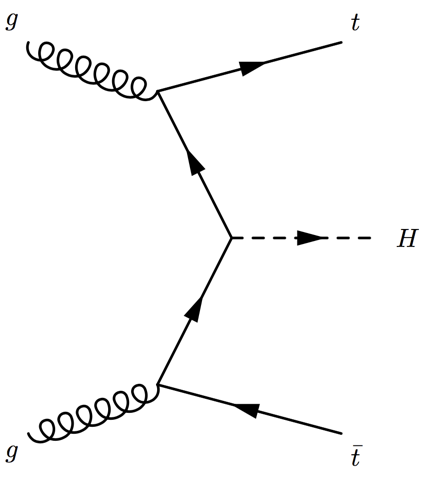
\includegraphics[width=0.4\linewidth]{figures/tth/tth_feynman.png}
    \caption{Tree-level production of a Higgs boson in association with a top quark-antiquark pair.}
    \label{fig:tth_feynman}
\end{figure} 

This is in fact the best method of \emph{directly} constraining the top quark Yukawa coupling at the LHC.
Indirect constraints on $y_\text{t}$ come from measurements of Higgs boson production via gluon fusion and \Hgg decay, both of which proceed primarily through a top quark loop, as in Fig. ~\ref{fig:hgg_feynman}.
However, these constraints are indirect because they make the assumption that no other BSM particles also contribute to the loops. 

Complementary methods of constraining $y_\text{t}$ include extraction from the shapes of kinematic distributions in \ttb events~\cite{CMS:2020qzr}, reporting a measured value of $y_\text{t} = 1.16^{+0.24}_{-0.35}$.
The uncertainty on $y_\text{t}$ is more than a factor of 2 less than that obtained with a measurement of \ttH (\Hgg)\footnote{One caveat is that the \ttH (\Hgg) result does not quote an actual value of $y_\text{t}$, but rather the \ttH cross section, which is proportional to the square of $y_\text{t}$.}, but does not rely on assumptions about the \Hgg branching ratio.

\subsection{Landscape of \ttH Measurements}
The first observation of the \ttH process was reported in 2018 by the CMS experiment~\cite{Sirunyan:2018hoz}, using 36 \fbinv of data from pp collisions at $\sqrt{s} = 13$ TeV.
The first observations of \ttH production in a single H decay channel (\Hgg) were reported by the CMS~\cite{tth_observation} and ATLAS~\cite{Aad:2020ivc} collaborations.
The CMS observation of \ttH (\Hgg) is detailed in the following sections of this thesis.



%\subsection{\ttH~Production as a Probe of the Top Quark Yukawa Coupling}


\section{Overview of Analysis Strategy} \label{sec:tth_analysis_strategy}
A measurement of the cross section times branching fration of \ttH (\Hgg)~production is performed by defining regions of the data which are highly enriched in \ttH events. These regions, called ``signal regions'', are constructed through a set of requirements placed on all candidate events. 
The requirements consist of two components: 
(1) a ``loose preselection'', which selects events with at least some of the expected decay products of the \ttH system and 
(2) a selection based on the output of a binary classification algorithm (called ``BDT-bkg''), trained to separate \ttH from the SM background processes. The loose preselection aims to maintain a very high signal efficiency (FIXME: CITE) and provides the phase space in which BDT-bkg is trained.
The BDT-bkg algorithm is trained on MC simulation of signal and background, as well as a data-driven description of some backgrounds. After training the BDT-bkg algorithm, signal regions are constructed by placing requirements on the output of BDT-bkg (on top of the preselection requirements).
Within these signal regions, signal and background models are constructed and a measurement of the \ttH cross section is calculated by performing a simultaneous fit to events in all of the signal regions. 
%Although the loose preselection maintains an efficiency of X\% (FIXME) on \ttH events, the SM background is still far too large to perform a precise measurement of the \ttH cross section. The output of BDT-bkg is then used to construct signal regions.
%
\subsection{The \Hgg Decay Mode}
The analysis targets \ttH events in which the Higgs boson decays into two photons (\Hgg). As the photon is a massless particle, it does not couple directly to the Higgs boson.
Instead, the dominant process through which the Higgs boson decays to two photons involves a top quark loop, as shown in Figure~\ref{fig:hgg_feynman}.
\begin{figure}[h!]
    \centering
    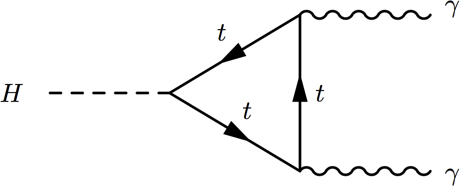
\includegraphics[width=0.6\textwidth]{figures/feynman_diagrams/hgg}
    \caption{To-do}
    \label{fig:hgg_feynman}
\end{figure}
The \Hgg branching ratio is quite small ($\approx 0.2\%$) in comparison to other commonly studied decay modes, but the diphoton channel presents several key advantages.

First, the CMS ECAL provides excellent energy resolution ($\sigma_E/E$) for reconstructed photons, which ranges from 1-5\% \cite{Chatrchyan:2013dga}.
In general, photons with smaller absolute values of pseudorapidity and higher values of the shower shape variable $R_9$ (defined in Section \ref{sec:evt_photon}) are reconstructed with better energy resolution.
The resulting resolution of the invariant mass of diphoton pairs then ranges from 1-2\% for events considered in this analysis.
Exact values for the mass resolution in each signal region are given in Section \ref{sec:sig_bkg_models}.
The mass resolution for other Higgs decay modes is typically much worse.
The CMS observation of the $\text{H} \to \text{b}\bar{\text{b}}$ decay mode, for example, achieved a mass resolution of 10-13\% \cite{Hbb_obs}.
The excellent mass resolution of the diphoton channel contributes to its competitive sensitivity -- the SM background follows a steeply falling distribution as a function of increasing diphoton invariant mass, while \Hgg events are clustered around \mH with a resolution of 1-2\%.
The narrow peak around \mH allows for greater discrimination against the SM background processes.


The second advantage of the diphoton decay channel is the relatively small SM background.
At the LHC, final states with photons or leptons are significantly rarer than final states with hadrons.
Each photon or lepton in a final state introduces another factor of the fine structure constant, $\alpha \approx 1/137$, in the cross section times branching ratio for a given process. 
A crude back of the envelope estimation suggests that final states with $N$ leptons plus photons have characteristic cross sections times branching ratios a factor of $\alpha^{-N}$ times smaller than characteristic cross sections times branching ratios for all-hadronic final states.


Finally, the diphoton decay channel has low systematic uncertainties in comparison to other Higgs decay modes.
Recent \ttH cross section measurements in multilepton and $\text{b}\bar{\text{b}}$ final states reported total systematic uncertainties of FIXME and CITE, while this result reports a systematic uncertainty of FIXME.
The fact that the uncertainty on measurements in the \Hgg channel are dominated by statistical uncertainties casts it as the ``golden channel'' for future Higgs studies in Run 3 of the LHC; the statistical uncertainty on measurements scales roughly with the inverse square root of the luminosity, while the systematic uncertainty remains roughly constant as a function of luminosity.


\section{Preselection} \label{sec:tth_presel}
Events passing the diphoton preselection, described in Sec.~\ref{sec:evt_photon_sel}, are eligible to enter one of two exclusive channels.
The hadronic channel targets \ttH events in which the \ttb pair decays fully hadronically, while the leptonic channel targets events in which at least one of the top (anti-)quarks decays leptonically.
The channels are defined to be orthogonal through selections on the number of leptons in the event: the leptonic channel requires at least one lepton and the hadronic channel requires exactly zero leptons.

Each channel then places an additional set of requirements on the events which enter.
The hadronic channel requires at least three jets, one of which must be identified as originating from a b quark.
Jets are identified as originating from a b quark using the DeepCSV b score, with a working point that corresponds to a 10\% misidentification rate for jets originating from light quarks or gluons.
The leptonic channel requires at least one jet, with no requirement on the jet flavor.


\section{Background Description} \label{sec:tth_background_description}
The analysis uses two methods of estimating the contribution of background processes (i.e., those other than \ttH).
The first estimates the background directly from data by fitting events in the \mgg sidebands, defined as $\mgg \in [100, 115] \cup [135, 180]$ GeV, by fitting a variety of functional forms.
The second estimates the background from individual descriptions of each background process.
These descriptions are taken primarily from simulations of each process; however, data-driven descriptions of some processes are also utilized: the multi-jet and \gjets backgrounds are described with a sample of events in data from the low photon ID sideband (described in Sec.~\ref{sec:tth_datadriven}).
The first method is referred to as the ``discrete profiling method'', while the second is referred to as the ``MC description'' of the background.

The discrete profiling method is used to estimate the background in the final statistical analysis and is described in Sec.~\ref{sec:tth_bkg_models}.
The MC description of the background is used only in designing and optimizing the cuts on the BDT-bkg algorithms and is described in this section.

\subsection{Challenges of MC Description} \label{sec:tth_mc_description}
The events entering the hadronic or leptonic preselection are dominated by Standard Model processes other than \ttH.
Precise knowledge of exactly which processes enter the preselection and their relative contributions to the overall background is not strictly necessary, as the background is modeled from events in data (described in Sec.~\ref{sec:tth_bkg_models}) when performing the measurement of $\mu_{\ttH}$.
However, the BDT-bkg algorithms are designed to distinguish between \ttH and the SM background processes; to this end, an accurate description of the background is desirable.
Note that events in data cannot be used to both model the background in the measurement of $\mu_{\ttH}$ and in training the BDT-bkg algorithm, as this would bias the measurement.
The starting point for the background description used in training the BDT-bkg algorithms is simulation of the relevant SM processes.
In the hadronic channel, the dominant backgrounds at preselection level are the multi-jet, \gjets, and \dipho processes; those same processes, as well as \ttbar, \ttg, \ttgg, and \Vgamma dominate for the leptonic channel.
The \mgg distribution for events in data and simulation are shown in Fig.~\ref{fig:tth_mgg_presel_datamc}.
The exact yields and relative contributions of all considered background processes are shown in Table~\ref{tab:tth_presel_datamc}.

\begin{figure} [h!]
    \centering
    \begin{tabular}{c c}
        \includegraphics[width=0.48\linewidth,page=1]{{figures/tth/ttHHadronic_RunII_MVA_Presel_v4.11_9Jun2020_no_scale_histogramsRunIIstd_linear}.pdf} &
        \includegraphics[width=0.48\linewidth,page=1]{{figures/tth/ttHLeptonic_RunII_MVA_Presel_v4.11_9Jun2020_histogramsRunIIstd_linear}.pdf} 
    \end{tabular}
    \caption{Diphoton invariant mass distributions for events from data and simulation entering the hadronic (right) and leptonic (left) channel preselections. Events in data are blinded in the region $\mgg \in [120, 130]$.}
    \label{fig:tth_mgg_presel_datamc}
\end{figure}

\begin{table} [h!]
    \centering
    \caption{Yields and fraction of total background by process for the hadronic (left) and leptonic (right) channel preselections. Backgrounds not explicitly shown in Fig.~\ref{fig:tth_mgg_presel_datamc} are consolidated in the ``Other'' category.}
    \begin{tabular}{c c}
    	\begin{tabular}{ r || r | r} \hline \hline
			Process & Yield & $\mathcal F$ of bkg \\ \hline
			\dipho & 40972.68 $\pm$ 75.87 & 0.32 \\ 
			\gjets & 52434.13 $\pm$ 1960.51 & 0.41 \\ 
			Multi-jet & 29277.57 $\pm$ 3566.18 & 0.23 \\ 
			\ttgg & 642.31 $\pm$ 35.09 & 0.01 \\ 
			\ttg & 1538.53 $\pm$ 68.77 & 0.01 \\ 
			\ttb & 997.19 $\pm$ 74.15 & 0.01 \\ 
			Drell-Yan & 265.24 $\pm$ 47.48 & 0.00 \\ 
			$\text{t} + \gamma$ & 170.79 $\pm$ 26.66 & 0.00 \\ 
			V + $\gamma$ & 1237.50 $\pm$ 39.10 & 0.01 \\ 
			\ttW & 3.13 $\pm$ 0.17 & 0.00 \\ 
			\ttZ & 3.41 $\pm$ 0.15 & 0.00 \\ 
			VV & 55.06 $\pm$ 4.49 & 0.00 \\ 
			tV & 135.61 $\pm$ 7.57 & 0.00 \\  \hline
			tHq & 5.53 $\pm$ 0.00 & 0.00 \\
            tHW & 1.44 $\pm$ 0.00 & 0.00 \\
			ggH & 199.20 $\pm$ 1.80 & 0.00 \\
            VH & 22.94 $\pm$ 0.22 & 0.00 \\
            VBF & 18.78 $\pm$ 0.24 & 0.00 \\ 
            All bkg. & 128029.09 $\pm$ 4072.22 & 1.00 \\ \hline 
            Data & 233060.00 $\pm$ 482.76 & 1.82 \\ \hline 
			\ttH & 48.03 $\pm$ 0.32 & 0.00 \\  \hline \hline
		\end{tabular}    
		&
		\begin{tabular}{ r || r | r} \hline \hline
			Process & Yield & $\mathcal F$ of bkg \\ \hline
            \dipho & 1067.40 $\pm$ 13.85 & 0.15 \\ 
			\gjets & 1070.57 $\pm$ 236.09 & 0.15 \\ 
			Multi-jet & 482.43 $\pm$ 343.91 & 0.07 \\ 
			\ttgg & 313.58 $\pm$ 8.39 & 0.04 \\ 
			\ttg & 542.93 $\pm$ 11.70 & 0.08 \\ 
			\ttb + Jets & 159.21 $\pm$ 6.15 & 0.02 \\ 
			Drell-Yan & 220.56 $\pm$ 39.78 & 0.03 \\ 
            $\text{t} + \gamma$ & 37.43 $\pm$ 13.28 & 0.01 \\ 
			V + $\gamma$ & 3081.67 $\pm$ 56.46 & 0.43 \\ 
			\ttW & 3.61 $\pm$ 0.18 & 0.00 \\ 
			\ttZ & 4.75 $\pm$ 0.17 & 0.00 \\ 
			VV & 51.79 $\pm$ 4.12 & 0.01 \\ 
			tV & 61.17 $\pm$ 4.88 & 0.01 \\  \hline
			tHq & 1.83 $\pm$ 0.00 & 0.00 \\ 
            tHW & 0.79 $\pm$ 0.00 & 0.00 \\ 
			ggH & 4.90 $\pm$ 0.25 & 0.00 \\ 
            VH & 10.67 $\pm$ 0.14 & 0.00 \\ 
            VBF & 0.74 $\pm$ 0.04 & 0.00 \\ \hline 
			All bkg. & 7138.36 $\pm$ 423.60 & 1.00 \\ \hline
			Data & 9450.00 $\pm$ 97.21 & 1.32 \\ \hline
			\ttH & 22.36 $\pm$ 0.21 & 0.00 \\  \hline \hline
		\end{tabular}
    \end{tabular}
    %\caption{Yields and fraction of total background by process for the hadronic (left) and leptonic (right) channel preselections. Backgrounds not explicitly shown in Fig.~\ref{fig:tth_mgg_presel_datamc} are consolidated in the ``Other'' category.}
	\label{tab:tth_presel_datamc}
\end{table}

In both channels, the overall yield from the background description given by simulation is somewhat smaller than what is observed in data.
This underprediction can be primarily attributed to a poor MC description of the multi-jet and \gjets processes, as the following section illustrates (and remedies). 

\subsection{Data-Driven Description of Multi-jet and \gjets Backgrounds} \label{sec:tth_datadriven}
To better understand the reason for the large discrepancies between data and simulation shown in Fig.~\ref{fig:tth_mgg_presel_datamc} and Table~\ref{tab:tth_presel_datamc}, it is helpful to study the discrepancy as a function of the event kinematics.
The distribution of minimum photon ID, defined as the smaller of the two photon ID BDT scores in the event, illustrates that the underprediction from simulation stems primarily from low values of minimum photon ID, as shown in Fig.~\ref{fig:tth_phoID_presel_datamc}.
\begin{figure} [h!]
    \centering
    \begin{tabular}{c c}
        \includegraphics[width=0.48\linewidth,page=42]{{figures/tth/ttHHadronic_RunII_MVA_Presel_v4.11_9Jun2020_no_scale_histogramsRunIIstd_linear}.pdf} &
        \includegraphics[width=0.48\linewidth,page=43]{{figures/tth/ttHLeptonic_RunII_MVA_Presel_v4.11_9Jun2020_histogramsRunIIstd_linear}.pdf}
    \end{tabular}
    \caption{Minimum photon ID distributions for events from data and simulation entering the hadronic (right) and leptonic (left) channel preselections. Events in data are blinded in the region $\mgg \in [120, 130]$.}
    \label{fig:tth_phoID_presel_datamc}
\end{figure}

The underprediction from simulation is especially pronounced at lower values of minimum photon ID, while the agreement becomes better for higher values. 
As the photon ID BDT discriminates between prompt and fake photons, we expect the lower end of the distribution to have a larger contribution from fake photons.
Thus, Fig.~\ref{fig:tth_phoID_presel_datamc} suggests that simulation provides an inadequate description of events with at least one fake photon. 

To improve the description of events with at least one fake photon (i.e. multi-jet and \gjets events), a sample of events from an orthogonal region of data is used in place of the simulation when training BDT-bkg.
This region, the ``low photon ID sideband'', is defined identically to the preselection except for the cut on minimum photon ID: the preselection requires minimum photon ID $>-0.7$, while the low photon ID sideband requires $-0.9<$ minimum photon ID $<-0.7$.
The preselection and low photon ID sideband are depicted in Fig.~\ref{fig:tth_low_photon_ID_sideband_pic}. 
\begin{figure} [h!]
    \centering
    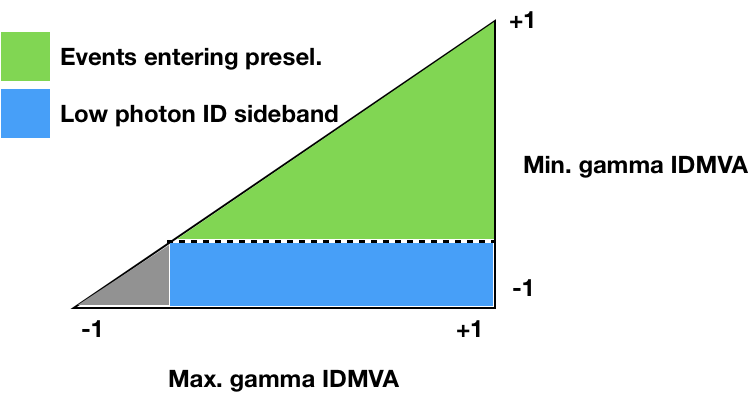
\includegraphics[width=0.75\linewidth]{{figures/tth/low_photon_ID_sideband.png}}
    \caption{Depiction of the relationship between preselection (green) and low photon ID sideband (blue).}
    \label{fig:tth_low_photon_ID_sideband_pic}
\end{figure}
Replacing the MC description of multi-jet and \gjets with the data-driven description relies on the assumption that events in the low photon ID sideband are exlusively multi-jet and \gjets events.
Simulation indicates that $> 95\%$ of events in the low photon ID sideband are multi-jet or \gjets events.

An immediate challenge in making the replacement of MC description of multi-jet and \gjets $\to$ data-driven description of multi-jet and \gjets is the fact that the minimum photon ID for these events and the minimum photon ID for events in the preselection are disjoint, by definition.
This is problematic because of the fact that minimum photon ID is used as a training feature for the BDT-bkg algorithms.
Training with an unaltered minimum photon ID distribution would lead the BDT to eliminate all of these background events with a single cut at the value of minimum photon ID that defines the sideband.
To make the data-driven sample feasible for use in training the BDT-bkg algorithm, its minimum photon ID distribution should be altered such that it resembles the expected distribution of multi-jet and \gjets events in the preselection region.

To generate the proper minimum photon ID distribution for events in the data-driven sample, the minimum photon ID score of each event is replaced by a randomly drawn value from a probability distribution function that describes the expected distribution of multi-jet and \gjets in the preselection.
The procedure is simplified by assuming that for events in the low photon ID sideband the photon with the lower photon ID score is always a fake photon.
This assumption is always true for multi-jet events (which have two fake photons), and from simulation, is found to be true for $> 95\%$ of \gjets events.
Under this assumption, the expected distribution of minimum photon ID for multi-jet and \gjets events in the preselection region can be approximated by the probability distribution function of photon ID for fake photons, called the ``fake pdf''.
The fake pdf is derived from simulation using the photon ID distribution of photons which are identified as fakes at generator-level.
For ease of drawing random values from this pdf, a histogram of the fake pdf is fitted with a seventh-order polynomial, shown in Fig.~\ref{fig:tth_fake_pdf}.
\begin{figure} [h!]
    \centering
    \includegraphics[width=0.75\linewidth]{{figures/tth/fake_photonID_shape.pdf}}
    \caption{Histogram of photon ID for fake photons in simulation (blue) and resulting seventh-order polynomial.}
    \label{fig:tth_fake_pdf}
\end{figure}
However, as minimum and maximum photon ID are strongly correlated by construction, the maximum photon ID distribution for events from the low photon ID sideband will also be different than the maximum photon ID distribution for events from the preselection.
In general, events from the low photon ID sideband will have lower maximum photon ID scores than events from the preselection.
To address the differences in maximum photon ID, an additional weight is applied to each event to correct for the fact that the distribution is biased towards lower values of maximum photon ID:
\begin{align} \label{eqn:impute_weight}
    w &= \frac{\int_{B}^{\text{max } \gamma \text{ ID}} \text{fake pdf}}{\int_{A}^{B} \text{fake pdf}} \\
    A &\equiv \text{minimum value of photon ID in the low photon ID sideband} = -0.9 \\
    B &\equiv \text{preselection cut value on minimum photon ID} = -0.7
\end{align} 
Qualitatively, the term of the numerator of Eqn.~\ref{eqn:impute_weight} increases the contribution of events from the low photon ID sideband with high values of maximum photon ID.
The term in the denominator is simply an overall normalization factor.
After applying the per-event weight, the overall normalization of the data-driven sample is determined with a simultaneous fit to data of the minimum and maximum photon ID distributions in the preselection.
The normalization of \dipho is also allowed to float in this fit, while the normalization of all other background processes are taken to be fixed.
\begin{figure} [htbp!]
    \centering
    \begin{tabular}{c c}
        \includegraphics[width=0.48\linewidth,page=42]{{figures/tth/ttHHadronic_RunII_MVA_Presel_v4.11_9Jun2020_impute_no_scale_histogramsRunIIstd_linear}.pdf} &
        \includegraphics[width=0.48\linewidth,page=43]{{figures/tth/ttHHadronic_RunII_MVA_Presel_v4.11_9Jun2020_impute_no_scale_histogramsRunIIstd_linear}.pdf} \\
		\includegraphics[width=0.48\linewidth,page=42]{{figures/tth/ttHHadronic_RunII_MVA_Presel_v4.11_9Jun2020_impute_histogramsRunIIstd_linear}.pdf} &
        \includegraphics[width=0.48\linewidth,page=43]{{figures/tth/ttHHadronic_RunII_MVA_Presel_v4.11_9Jun2020_impute_histogramsRunIIstd_linear}.pdf} \\
    \end{tabular}
    \caption{Distributions of minimum (left) and maximum (right) photon ID in the hadronic preselection before (top) and after (bottom) fitting the normalization of the data-driven description of multi-jet and \gjets and the MC description of \dipho.}
    \label{fig:tth_phoID_fits}
\end{figure}

\begin{table} [h]
	\centering
	\caption{Results of binned fit of diphoton templates in the hadronic preselection, with template for prompt/prompt taken from MC simulation and template for fake/fake and fake/prompt taken from the data-driven description.}
	\begin{tabular}{|l|| r| r| r|} \hline
		Template & Initial Fraction & Fitted Fraction & Scale \\ \hline
		$ \gamma $ + jets (fake/prompt) & 0.68 & 0.73 $ \pm $ 0.00 & 1.07 \\
		$ \gamma \gamma $ + jets (prompt/prompt) & 0.18 & 0.25 $ \pm $ 0.00 & 1.42 \\ \hline
	\end{tabular}
	%\caption{Results of binned fit of diphoton templates in the hadronic preselection, with template for prompt/prompt taken from MC simulation and template for fake/fake and fake/prompt taken from the data-driven description.}
    \label{tab:tth_phoID_fits}
\end{table}
The minimum and maximum photon ID distributions are shown pre-/post-fit in Fig.~\ref{fig:tth_phoID_fits} and the results of the fit are shown in Table~\ref{tab:tth_phoID_fits}.
The agreement with data is significantly improved when using the data-driven description of multi-jet and \gjets in place of the MC description, as can be seen by comparing Fig.~\ref{fig:tth_phoID_presel_datamc} and Fig.~\ref{fig:tth_phoID_fits}.
This improvement is consistently seen in other distributions as well, including the jet and b-jet multiplicities shown in Fig.~\ref{fig:tth_impute_compare}.
\begin{figure} [htbp!]
    \centering
    \begin{tabular}{c c}
        \includegraphics[width=0.48\linewidth,page=5]{{figures/tth/ttHHadronic_RunII_MVA_Presel_v4.11_9Jun2020_no_scale_histogramsRunIIstd}.pdf} &
        \includegraphics[width=0.48\linewidth,page=5]{{figures/tth/ttHHadronic_RunII_MVA_Presel_v4.11_9Jun2020_impute_histogramsRunIIstd}.pdf} \\
        \includegraphics[width=0.48\linewidth,page=8]{{figures/tth/ttHHadronic_RunII_MVA_Presel_v4.11_9Jun2020_no_scale_histogramsRunIIstd}.pdf} &
        \includegraphics[width=0.48\linewidth,page=8]{{figures/tth/ttHHadronic_RunII_MVA_Presel_v4.11_9Jun2020_impute_histogramsRunIIstd}.pdf} \\
    \end{tabular}
    \caption{Agreement between data and MC description of background for jet multiplicity (top) and b-jet multiplicity (bottom), shown with both the MC description of multi-jet and \gjets (left) and the data-driven description of multi-jet and \gjets (right).} 
    \label{fig:tth_impute_compare}
\end{figure}
%Using events from the low photon ID sideband to describe the multi-jet and \gjets processes relies on several assumptions:
%\begin{enumerate}
%    \item The low photon ID sideband is composed completely of multi-jet and \gjets events.
%    \item The photon with the smaller photon ID value is always a fake photon.
%    \item The output of photon ID BDT is uncorrelated with other input features used in training the BDT-bkg algorithms.
%\end{enumerate}

As the MC description of the background is used only for designing and optimizing the cuts on the BDT-bkg algorithms, the bottom-line test of the merit of the data-driven description is BDT-bkg performance.
To this end, we compare the performance of the BDT-bkg algorithm trained with the MC description of \gjets (including the MC description of multi-jet events was found to degrade performance because of the extremely few number of events from the multi-jet simulation samples) with the performance of the BDT-bkg algorithm trained with the data-driven description of multi-jet and \gjets, using $Z_A$ (defined in Sec.~\ref{sec:tth_za}) as an estimate of the expected signifiance obtained when using either BDT.
$Z_A$ is shown for each BDT as a function of the number of \ttH events in Fig.~\ref{fig:tth_imputing_za}.
The improvement obtained by replacing the MC description of \gjets with the data-driven description of multi-jet and \gjets, taken as the percentage difference between the maximum $Z_A$ values obtained with either method, is about 8\%.
\begin{figure} [h!]
    \centering
    \includegraphics[width=0.75\linewidth]{{figures/tth/za_comparison_data_imputing_vs_scale_mc_12Apr2020.pdf}}
    \caption{Expected significance ($Z_A$) shown as a function of the number of \ttH events passing a given cut on BDT-bkg for versions of BDT-bkg trained with the MC description of \gjets (black) and the data-driven description of multi-jet and \gjets (red). Shaded bands show the $\pm 1\sigma$ statistical uncertainty in $Z_A$.}
    \label{fig:tth_imputing_za}
\end{figure}
The data-driven description of multi-jet and \gjets events is not employed in the leptonic channel as it was not found to significantly improve BDT-bkg performance.
This is likely due to the combination of two factors:
\begin{enumerate}
    \item Events in the leptonic low photon ID sideband are not dominated by multi-jet and \gjets events to the same extent as in the hadronic channel; \ttbar and \ttg events play a significant role as well.
    \item The multi-jet and \gjets processes make up a smaller overall fraction of the background contribution in the leptonic preselection; there is a lower ceiling on improvements to BDT-bkg performance from improved description of these processes.
\end{enumerate}


\section{Machine Learning Algorithms} \label{sec:tth_mvas}
The analysis strategy relies on the use of a binary classification algorithm to create regions of high \ttH purity.
A boosted decision tree (BDT) is chosen as the binary classification algorithm.
Deep neural networks (DNNs) were also explored; however, these were found to outperform BDTs only when a very high number of training examples are available (discussed in further detail in Sec.~\ref{sec:tth_dnns}).
The BDT-bkg algorithms are trained with the \textsc{xgboost}~\cite{xgboost} framework, using MC simulation of \ttH for the signal events and a combination of MC simulation and data-driven descriptions of the relevant background processes as background.
In order to avoid bias, the BDT-bkg algorithms are trained and optimized on completely separate samples from those used in the measurement of $\mu_{\ttH}$.
The various background processes are weighted according to their cross sections, while the weights of signal events are scaled such that the total number of signal events is equal to the total number of background events.
The signal weights are scaled in such a fashion to avoid issues in training related to imbalanced classes.
The features used in training the BDT-bkg algorithms are discussed in the following subsections. 

\subsection{High-Level Features} \label{sec:tth_hlf}
In order to effectively separate \ttH from the SM backgrounds, we construct a number of high-level physics variables which are expected to have discriminating power between the two.
The full list of features is shown in Table~\ref{tab:tth_hlf}.
Plots showing the distributions for both data and simulation for each input feature are shown in Appendix~\ref{app:hlf}.

\begin{table}[h] \scriptsize
\centering
\caption{High level features used in training BDTs. The fourth jet kinematics are given as input features only to the BDT-bkg in the hadronic channel, while the lepton kinematics are given as input features only to the BDT-bkg in the leptonic channel.} 
\renewcommand{\arraystretch}{1.5}
\begin{tabular}{|c| c c c|}
\multicolumn{4}{c}{Input Features to BDTs} \\ \hline
Category & \multicolumn{3}{c|}{Features} \\ \hline
\multirow{3}{*}{Photon Kinematics} & $\gamma_1$ $p_T$/$m_{\gamma \gamma}$ & $\gamma_1$ $\eta$ & $\gamma_1$ Pixel Seed Veto \\
& $\gamma_2$ $p_T$/$m_{\gamma \gamma}$ & $\gamma_2$ $\eta$ & $\gamma_2$ Pixel Seed Veto \\
& Max $\gamma$ ID MVA & Min $\gamma$ ID MVA & \\ \hline
\multirow{7}{*}{Jet Kinematics} & Jet 1 $p_T$ & Jet 1 $\eta$ & Jet 1 b-tag score \\
& Jet 2 $p_T$ & Jet 2 $\eta$ & Jet 2 b-tag score \\
& Jet 3 $p_T$ & Jet 3 $\eta$ & Jet 3 b-tag score \\
& Jet 4 $p_T$ & Jet 4 $\eta$ & Jet 4 b-tag score \\
& Max b-tag score & 2nd max b-tag score & \\
& $N_{\text{jets}}$ & $H_T$ & \\ \hline
\multirow{2}{*}{DiPhoton Kinematics} & $p_T^{\gamma \gamma} / m_{\gamma \gamma}$ & $Y_{\gamma \gamma}$ & $|\cos (\Delta \phi)_{\gamma \gamma}|$ \\
& $\Delta R_{\gamma \gamma}$ & $|\cos(\text{helicity angle} (\theta))|$ & \\ \hline
Lepton Kinematics & lepton $p_T$ & lepton $\eta$ & $N_{\text{leptons (tight ID)}}$ \\ \hline
\multirow{1}{*}{Event-level Kinematics} & $E_T^{\text{miss}}$ & & \\ \hline
\end{tabular}
%\caption{High level features used in training BDTs. The fourth jet kinematics are given as input features only to the BDT-bkg in the hadronic channel, while the lepton kinematics are given as input features only to the BDT-bkg in the leptonic channel.} 
\label{tab:tth_hlf}
\end{table}

The physics motivations for the inclusion of each feature are enumerated below:
\begin{enumerate}
    \item Photon Kinematics
    \begin{itemize}
        \item Photon \pT divided by \mgg: prompt photons tend to have higher transverse momentum than fake photons from hadronic jets. The photon \pT is normalized by \mgg to prevent the BDT from learning \mH.
        \item Photon $\eta$: prompt photons tend have smaller $|\eta|$ than fake photons.
        \item Photon pixel seed veto: \ttplusX events often have one or more electrons from leptonically decaying \PW bosons which are identified as photons at reco-level. The pixel seed veto helps identify these events.
        \item Photon ID MVA: the primary means of separating between prompt and fake photons. Described in further detail in Sec.~\ref{sec:evt_photon_idmva}.
    \end{itemize}
    \item Jet Kinematics
    \begin{itemize}
        \item Jet \pT: jets from \ttH events tend to have higher transverse momentum than those from background processes (both multi-jet + X and \ttplusX), as the \ttb system recoils against the Higgs.
        \item Jet $\eta$: jets from \ttH tend to be more central than those from multi-jet + X events.
        \item Jet b-tag scores: jets from \ttH have higher b-tag scores than those from non-\ttb backgrounds, as two b-jets are expected 2 from the \ttb decay. 
        \item Number of jets: we expect at least 6 (4) jets in a \ttH event in the Hadronic (Leptonic) channel.
        \item $H_{\text{T}}$: \ttH events tend to have higher values of $H_{\text{T}}$, due to the fact that we expect higher $p_T$ of individual jets as well as more total jets in the event.
    \end{itemize}
    \item DiPhoton Kinematics
    \begin{itemize}
        \item DiPhoton \pT divided by \mgg: the recoil of the Higgs against the \ttb system results in higher expected values for the diphoton momentum. The DiPhoton \pT is normalized by \mgg to prevent the BDT from learning \mH.
        \item DiPhoton $Y$: the DiPhoton rapidity is expected to be closer to zero for \ttH events.
        \item DiPhoton $\Delta R$: the angle between the two photons is expected to be smaller for \ttH events due to the fact that the Higgs tends to be boosted from recoil against the \ttb system.
        \item Helicity angle ($\theta$): defined by boosting to the rest frame of the DiPhoton pair and calculating the angle between the photons in that frame. Since the SM Higgs is a scalar, we expect a uniform distribution in $\cos(\theta)$ for \ttH (at generator-level), while backgrounds may peak closer to 1.
        \item $\cos (\Delta \phi)$ of DiPhoton pair: similar argument to above.
    \end{itemize}
    \item Lepton Kinematics
    \begin{itemize}
        \item Lepton \pT: prompt leptons tend to have higher \pT than fake leptons from hadronic jets.
        \item Lepton $|\eta|$: prompt leptons tend to be more central than fake leptons.
        \item Number of leptons passing tight ID: again, helpful in discriminating between prompt and fake leptons. The preselection requires that leptons pass medium ID, the number of leptons passing tight ID is given as an input to the BDT.
    \end{itemize}
    \item Event-level Kinematics
    \begin{itemize}
        \item \met: in the Leptonic channel, we expect nonzero \met in \ttb events due to the neutrino from the $\PW\to l\nu$ decay, while no \met is expected for multi-jet + X events. In the Hadronic channel, this may also be useful in identifying leptonically decaying \ttH events in which the lepton is not reconstructed.
    \end{itemize}
\end{enumerate}

\subsection{Deep Neural Networks for \dipho and \ttgg Backgrounds} \label{sec:tth_dnns}
The dominant SM backgrounds in regions of high \ttH purity (i.e. similar to the signal regions) are: \dipho and \ttgg in the hadronic channel, and \ttgg in the leptonic channel.
To further reduce these backgrounds, additional methods and variables designed to specifically target these backgrounds were explored.
Among the most successful of these methods were deep neural networks (DNNs) trained to reject these backgrounds specifically.
Another notable susccessful tool is the top tagger BDT, discussed in Sec.~\ref{sec:tth_top_tagger_bdt}.

The DNNs exploit low-level information in each event which is lost in the process of summarizing the event in terms of the high-level features described in Sec.~\ref{sec:tth_hlf}.
An example of such low-level information is the azimuthal angle $\phi$ of the reconstructed jets and leptons.
Any physics process should obey azimuthal symmetry in the CMS detector -- any value of $\phi$ is equally likely for any physics object from any physics process.
For this reason, the $\phi$ value of a given jet or lepton on its own provides no means to discriminate between \ttH and other SM backgrounds.
However, the $\phi$ value of a jet or lepton may provide discriminatory power when considered in the context of the rest of the event: angles between jets and leptons likely have different distributions in \ttH events and SM background events.
Providing this type of low-level input to a BDT would be of limited use, as making a splitting on the $\phi$ value of a jet or lepton is not useful on its own.
Deep neural networks were then explored as an algorithm which could potentially make better use of such low-level features.

\subsubsection{Training Features}
The high-level features described in Sec.~\ref{sec:tth_hlf} do not retain the full information of the original event.
To provide a more complete description of each event, the four-vectors of the leading jets and leptons (``physics objects'') are given as inputs to the DNNs.
The four-vector includes the physics object's \pT, $\eta$, $\phi$, and total energy ($E$).
In addition to the four-vectors, four jet flavor scores and lepton ID flags, indicating whether a given lepton is a muon or electron are provided for each physics object.
In total, for up to the leading eight (six) jets in each event and the leading zero (two) leptons in each event in the Hadronic (Leptonic) channel, the following nine features are provided for each physics object:
\begin{itemize}
    \item Four-vector: $p_T$, $\eta$, $\phi$, $E$
    \item 4 DeepCSV scores: $b$, $c$, $udsg$, $bb$
    \item Lepton ID flag: 0 for muons, 1 for electrons
\end{itemize}
In the hadronic channel, there are no leptons and so the Lepton ID flag is omitted, resulting in 8 features per physics object.
In the leptonic channel, jets (leptons) are assigned `dummy'' values for the lepton ID flag (DeepCSV scores) of -2.
The "dummy" values are necessary as each physics object that is input to the DNN must have the same number of input features.
Photons are not included in the list of physics objects to prevent the DNN from learning \mH.

In addition to the low-level object features, a set of high-level features, shown in Table~\ref{tab:tth_hlf_dnn}, is given as inputs to the DNN to allow it to learn correlations between the physics objects and the rest of the event, including the diphoton kinematics and missing transverse momentum.
\begin{table}[h] \scriptsize
	\centering
	\caption{High level features used in training DNNs. The lepton kinematics features are only given as inputs to the leptonic channel DNN.} 
	\renewcommand{\arraystretch}{1.5}
	\begin{tabular}{c| c c c c}
		\multicolumn{5}{c}{High-level features for DNNs} \\ \hline
		Category & \multicolumn{4}{c}{Features} \\ \hline
		\multirow{3}{*}{Photon Kinematics} & $\gamma_1$ \pT/\mgg & $\gamma_1$ $\eta$ & $\gamma_1$ $\phi$ & $\gamma_1$ Pixel Seed Veto \\
		& $\gamma_2$ \pT/\mgg & $\gamma_2$ $\eta$ & $\gamma_2$ $\phi$ & $\gamma_2$ Pixel Seed Veto \\
		& Max $\gamma$ ID MVA & Min $\gamma$ ID MVA & & \\ \hline
		\multirow{2}{*}{Jet Kinematics} & Max b-tag score & 2nd max b-tag score & & \\
		& $N_{\text{jets}}$ & & & \\ \hline
		\multirow{1}{*}{DiPhoton Kinematics} & $\pT^{\gamma \gamma} / \mgg$ & $Y_{\gamma \gamma}$ & $\Delta R_{\gamma \gamma}$ & \\ \hline
		\multirow{1}{*}{Lepton Kinematics} & $N_{\text{leptons (tight ID)}}$ & & & \\ \hline
		\multirow{1}{*}{Event-level Kinematics} & \met & $\met \phi$ & & \\ \hline
	\end{tabular}
	%\caption{High level features used in training DNNs. The lepton kinematics features are only given as inputs to the leptonic channel DNN.} 
	\label{tab:tth_hlf_dnn}
\end{table}

\subsubsection{Architecture}
Arguably the simplest approach would be to feed the low-level and high-level features to a fully-connected deep neural network.
However, the question arises of how to organize the physics objects in the event: how does one identify the ``first'' jet in an event?
One solution is to order the physics objects by their \pT, meaning that the first jet in the event is the one with the highest \pT.
This strategy is far from perfect: in some \ttH events the first jet may be a b jet from a top decay, while in others the first jet may be a c jet from a \PW decay.
A long-short term memory (LSTM) architecture~\cite{lstm} is employed to address this challenge.
The physics objects are treated as a one-dimensional sequence (ordered by \pT) that is given to the LSTM.
This choice of architecture is motivated by other successful applications of LSTMs to physics objects, notably the DeepCSV and DeepJet architectures which classify jet flavor in part from a one-dimensional sequence of PF candidates given to an LSTM.
The output of the LSTM network is then merged with the high-level features in a set of fully-connected layers, as depicted in Fig.~\ref{fig:tth_dnn_diagram}.
\begin{figure}[h]
    \centering
    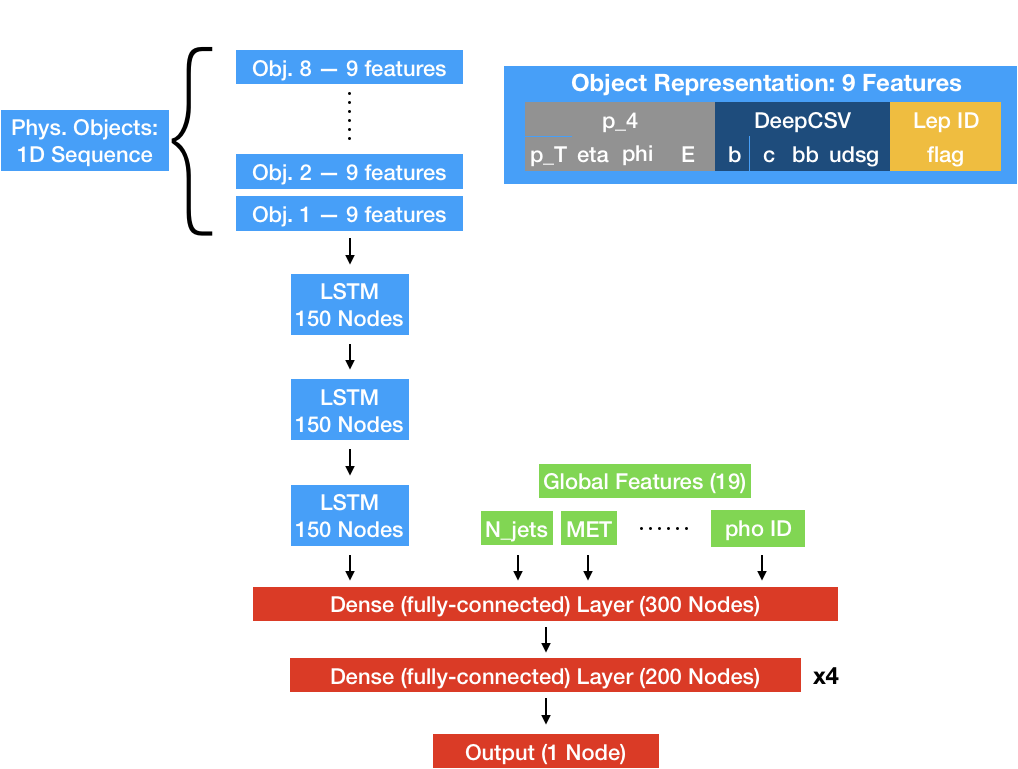
\includegraphics[width=0.7\linewidth]{figures/tth/leptonic_dnn_diagram.png}
    \caption{Schematic of deep neural network architecture, shown for the leptonic channel.}
    \label{fig:tth_dnn_diagram}
\end{figure}

\subsubsection{Training Details}
The DNN is implemented in \texttt{keras}~\cite{keras} with \texttt{tensorflow}~\cite{tensorflow} backend.
It uses the Adam optimizer~\cite{adam} with a learning rate of of $10^{-3}$ and with a binary cross-entropy loss function.
It is trained with an early-stopping procedure in which the batch size is increased over the course of training~\cite{increase_batch}.
Starting with a batch size of 1024, the DNN is trained until the improvement in 1-AUC, as calculated on the validation set, after each epoch is less than 1\%, at which point the batch size is quadrupled.
This procedure is repeated until the batch size exceeds 50,000, at which point it is capped and the training is stopped when the validation AUC ceases to improve.
The batch size is capped due to technical limitations of the GPU: large batch sizes take up a large amount of memory.
DNN hyperparameters are summarized in Table~\ref{tab:tth_dnn_hyperparams}.

\begin{table} [h]
    \centering
    \caption{Hyperparameters for the deep neural networks used in both the hadronic and leptonic channels.}
    \begin{tabular}{l l}
        Hyperparameter & Value(s) \\ \hline
        Number of nodes (fully connected layers) & 300, 200, 200, 200, 200 \\
        Number of nodes (LSTM layers) & 150, 150, 150 \\
        L2-normalization constraint (``maxnorm'') & 3 \\
        Dropout rate & 0.1 \\
        Learning rate & $10^{-3}$ \\
        Batch momentum & 0.99 \\
        Activation function (LSTM) & hyperbolic tangent \\
        Activation function (fully-connected layers) & exponential linear unit \\
        Activation function (output layer) & sigmoid \\
    \end{tabular}
    %\caption{Hyperparameters for the deep neural networks used in both the hadronic and leptonic channels.}
    \label{tab:tth_dnn_hyperparams}
\end{table}

A number of regularization methods are employed, which were found to improve performance and/or convergence speed during training.
First, training features are preprocessed with a `Z-score'' normalization procedure, subtracting the mean and dividing by the standard deviation of each feature such that all features have zero mean and unit variance.
In addition to the Z-score transformation, input features with units of GeV are given in terms of their logarithm, with the log taken before the Z-score transformation.
The aim of preprocessing is to provide a uniform scale for all input features, as this results in faster convergence during training and even improved performance~\cite{lecun_efficient_backprop}.
In the same spirit as feature preprocessing, batch normalization~\cite{ioffe2015batch} is applied between the fully-connected layers of the DNN, normalizing each layer's inputs.
Batch normalization is not applied in between the LSTM layers.
Both feature preprocessing and batch normalization resulted in faster convergence and improved performance of the DNNs.
In addition, dropout~\cite{dropout} is applied between the fully-connected layers in order to reduce overfitting and improve performance.
Between layers which apply both batch normalization and dropout, batch normalization is applied first and dropout is applied second.

\subsubsection{Performance}
Three separate DNNs are trained:
\begin{itemize}
    \item Hadronic channel: \ttH vs. \dipho
    \item Hadronic channel: \ttH vs. \ttgg
    \item Leptonic channel: \ttH vs. \ttgg
\end{itemize}
The output of each DNN is shown for both data and simulation in Fig.~\ref{fig:tth_dnn_datamc}.
\begin{figure} [htbp!]
    \centering
    \begin{tabular}{c c}
        \includegraphics[width=0.48\linewidth,page=62]{{figures/tth/ttHHadronic_RunII_MVA_Presel_v4.11_9Jun2020_impute_histogramsRunIIstd}.pdf} &
        \includegraphics[width=0.48\linewidth,page=63]{{figures/tth/ttHHadronic_RunII_MVA_Presel_v4.11_9Jun2020_impute_histogramsRunIIstd}.pdf} \\
        \includegraphics[width=0.48\linewidth,page=73]{{figures/tth/ttHLeptonic_RunII_MVA_Presel_v4.11_9Jun2020_histogramsRunIIstd}.pdf} &
    \end{tabular}
    \caption{Agreement between data and MC description of background for the various DNNs used as input features to BDT-bkg, for the hadronic channel (top) and the leptonic channel (bottom).}
    \label{fig:tth_dnn_datamc}
\end{figure}
The DNNs are used as inputs to the BDT-bkg, rather than in place of the BDT-bkg because superior performance from DNNs was only observed in the case of a high number of events available for training.
The simulation samples describing \ttH, \dipho, and \ttgg processes each have a high number of individual events ($\geq 10^5$) passing the preselection requirements, so DNNs are trained to distinguish between these processes.
The improvement brought to each channel by the DNNs is shown in Fig.~\ref{fig:tth_dnn_za}.
\begin{figure} [htbp!]
    \centering
    \begin{tabular}{c c}
        \includegraphics[width=0.48\linewidth]{figures/tth/za_comparison_data_Hadronic_DNN_2May2020.pdf} &
        \includegraphics[width=0.48\linewidth]{figures/tth/za_comparison_data_Leptonic_DNN_2May2020.pdf}
    \end{tabular}
    \caption[Expected significance ($Z_A$) shown as a function of the number of \ttH events passing a given cut on BDT-bkg for versions of BDT-bkg trained with (red) and without (black) the DNN scores as training features.]{Expected significance ($Z_A$) shown as a function of the number of \ttH events passing a given cut on BDT-bkg for versions of BDT-bkg trained with (red) and without (black) the DNN scores as training features. Shaded bands show the $\pm 1\sigma$ statistical uncertainty in $Z_A$. The background yield is estimated from events in data in the \mgg sidebands.}
    \label{fig:tth_dnn_za}
\end{figure}
The improvement in expected sensitivity in the hadronic channel is about 10\%.
The improvement in the leptonic channel is significantly smaller than the statistical uncertainty in $Z_A$.
The fact that the improvement is greater in the hadronic channel is likely attributed to the fact that it benefits from the DNN trained against the \dipho background.
Not only is this the largest background in the \ttH hadronic channel signal regions, but the simulation sample has the largest number of events entering the preselection, allowing for aggressive DNN training with lower risk of overfitting.

\subsection{Top Tagger BDT} \label{sec:tth_top_tagger_bdt}
The dominant backgrounds in the hadronic channel at both preselection level and signal region level are the multi-jet, \gjets, and \dipho processes.
An obvious difference between these processes and \ttH is the fact that there are two top (anti-)quarks in the latter, while there are none in the former.
This motivates the use of methods which can identify the presence of top quarks as a tool for further rejecting the multi-jet, \gjets, and \dipho backgrounds.

The chosen method is a top tagger BDT, originally developed in a search for supersymmetric partners of the top quark~\cite{stop_search} and later updated for \ttH.
The BDT is trained using \textsc{xgboost}~\cite{xgboost}.
The BDT takes jet triplets as inputs, with triplets that are matched as coming from a top quark (using generator truth-level information) designated as signal and all other triplets designated as background.
Jets are required to have $p_T > 25$ GeV and $|\eta| < 2.4$.
In addition, the jets are cleaned such that they are not overlapping with leptons.
The truth matching enforces the following additional requirements:
\begin{itemize}
    \item $|m_{jjj} - m_t| < 80$ GeV
    \item All three reco jets are matched to generator-level quarks from a hadronically decaying top ($\Delta R(\text{jet, quark}) < 0.4$).
\end{itemize}
The training features are shown in Table \ref{tab:tth_top_tagger_features}.
\begin{table}
	\centering
    \caption{Input features used in training the Top Tagger BDT.}
	\begin{tabular}{c |c c c c} \hline \hline
		Category & \multicolumn{4}{c}{Features} \\ \hline
		\multirow{3}{*}{Single Jet Quantities} & $p_T$ & mass & & \\
		& DeepCSV b & DeepCSV c vs. light & DeepCSV c vs. b & \\
		& ptD & axis1 & multiplicity & \\ \hline
		\multirow{1}{*}{Di-Jet Quantities} & $\Delta R(\text{j,j})$ & $m_{\text{jj}}$ & & \\
		\multirow{1}{*}{Tri-Jet Quantities} & $\Delta R(\text{b,W})$ & $m_{\text{jjj}}$ & &  \\ \hline \hline
	\end{tabular}
    %\caption{Input features used in training the Top Tagger BDT.}
    \label{tab:tth_top_tagger_features}
\end{table}
The training features are defined as follows:
\begin{itemize}
    \item DeepCSV scores: for each jet, three DeepCSV quantities are provided: the b-tag score, and the c-tag score, given in terms of c vs. light and c vs. b.
    \item ptD, axis1, multiplicity: standard quark-gluon discrimination variables. The fragmentation function is defined as $\text{ptD} \equiv \frac{\sqrt{\sum p_{\text{T}_i}^2}}{\sum p_{\text{T}_i}}$, axis1 is the jet shape variable describing the jet's long axis, and multiplicity provides the number of constituents in the jet.
\end{itemize}
The jet in the triplet with the highest DeepCSV b score is labeled as the b-jet, while the other two jets are labeled as $\PW$-jet 1 and 2, with $\pT(\PW_{j1}) > \pT(\PW_{j2})$.

The ouput of the top tagger BDT is shown for both data and simulation in Fig.~\ref{fig:tth_top_tagger_datamc}.
\begin{figure} [htbp!]
    \centering
    \includegraphics[width=0.48\linewidth,page=48]{{figures/tth/ttHHadronic_RunII_MVA_Presel_v4.11_9Jun2020_impute_histogramsRunIIstd}.pdf}
    \caption{Agreement between data and MC description of background for the top tagger BDT score.}
    \label{fig:tth_top_tagger_datamc}
\end{figure}
Similar to the DNN scores, the top tagger BDT is given as an additional training feature to BDT-bkg.
The improvement in expected sensitivity gained by adding the top tagger to BDT-bkg is shown in Fig.~\ref{fig:tth_top_tagger_za} and is about 5\%.
\begin{figure} [htbp!]
    \centering
    \includegraphics[width=0.7\linewidth]{{figures/tth/za_comparison_data_Hadronic_TopTagger_2May2020}.pdf}
    \caption[Expected significance ($Z_A$) shown as a function of the number of \ttH events passing a given cut on BDT-bkg for versions of BDT-bkg trained with (red) and without (black) the top tagger BDT scores as a training feature.]{Expected significance ($Z_A$) shown as a function of the number of \ttH events passing a given cut on BDT-bkg for versions of BDT-bkg trained with (red) and without (black) the top tagger BDT as a training feature. Shaded bands show the $\pm 1\sigma$ statistical uncertainty in $Z_A$. The background yield is estimated from events in data in the \mgg sidebands.}
    \label{fig:tth_top_tagger_za}
\end{figure}

\subsection{BDT-bkg}
The final BDT-bkg algorithms for each channel use the high-level features listed in Table~\ref{tab:tth_hlf}, the DNN scores described in Sec.~\ref{sec:tth_dnns}, and the top tagger BDT score described in Sec.~\ref{sec:tth_top_tagger_bdt} as the training features.
The outputs of the BDT-bkg algorithms are shown in Fig.~\ref{fig:tth_bdt-bkg}, where agreement between data and simulation is observed within statistical and systematic uncertainties.
\begin{figure} [htbp!]
    \centering
    \begin{tabular}{c c}
        \includegraphics[width=0.48\linewidth]{figures/tth/Figure_001-a.pdf} &
        \includegraphics[width=0.48\linewidth]{figures/tth/Figure_001-b.pdf}
    \end{tabular}
    \caption[Output of the BDT-bkg algorithm for the hadronic channel (left) and the leptonic channel (right). Taken from~\cite{tth_observation}.]{Output of the BDT-bkg algorithm for the hadronic channel (left) and the leptonic channel (right). Events from the \mgg sidebands are shown for both data and simulation. The statistical (statistical $\oplus$ systematic) uncertainties in simulation are shown with black (red) shaded bands. The thinly dashed lines show the boundaries of each signal region used for the cross section measurement, while the thickly dashed lines show the boundaries of signal regions used for a measurement of the CP structure. Events in the gray shaded region are discarded. Taken from~\cite{tth_observation}.}
    \label{fig:tth_bdt-bkg}
\end{figure}

\subsubsection{Validation in \ttZ Events}
As an additional check of the agreement between data and simulation in the output of the BDT-bkg algorithms, a validation in a control region targeting \ttZ (\Zee) events is performed.
The rationale for using \ttZ events is the following: \ttZ and \ttH should have very similar kinematic distributions for most components.
Therefore, BDT-bkg should similarly assign high scores to \ttZ events as it does for \ttH events and a region of high \ttZ purity should be present at high scores.
Because the cross section times branching fraction of \ttZ (\Zee) is much higher than that of \ttH (\Hgg), this control region provides a test of the agreement between data and simulation for high scores of BDT-bkg with much smaller statistical uncertainty than obtained in the \mgg sidebands.
Lastly, it is important to emphasize that this check is qualitative in nature; no formal estimate of the compatibility between the distributions in data and simulation is performed.

The selection for the \ttZ control region is the same as the preselection, with the exception that the cut on the conversion-safe electron veto is inverted to select for \Zee events.
The reconstructed ``diphoton pairs'' in these events are then primarily composed of electrons that were reconstructed as photons.

Additional cuts are next applied on top of the preselection in order to increase the \ttZ purity:
\begin{itemize}
    \item $|m_{\text{Z}} - m_{\gamma \gamma}| < 10$ GeV
    \item $N_{\text{jets}} \geq 5 (3)$ for hadronic (leptonic)
    \item $N_{\text{b-jets}} \geq 2$, using the tight (medium) working point for hadronic (leptonic)
\end{itemize}

One subtlety in validating the BDT-bkg performance in \ttZ events is the fact that BDT-bkg is specifically trained to reject events in which electrons are reconstructed as photons through use of the pixel seed veto (defined in Sec.~\ref{sec:evt_photon_vardef}).
This challenge is addressed by manually changing the value of the pixel seed veto for these events before evaluating their score with the BDT-bkg algorithm: although most of these events fail the pixel seed veto, BDT-bkg is told that they all pass the pixel seed veto.
This hard-coding of the pixel seed veto ensures that \ttZ events are not assigned lower scores due to the fact that the typical diphoton pair in these events is suspiciously electron-like.

Comparisons of BDT-bkg between data and simulation are shown for events entering the \ttZ control regions in Fig.~\ref{fig:tth_bdt-bkg_ttz}.

\begin{figure} [htbp!]
    \centering
    \begin{tabular}{c c}
        \includegraphics[width=0.48\linewidth]{figures/tth/ttHHadronic_MVA_ttZ_12Jun2020.pdf}
        \includegraphics[width=0.48\linewidth]{figures/tth/ttHLeptonic_MVA_ttZ_12Jun2020.pdf}
    \end{tabular}
    \caption{Output of the BDT-bkg algorithm for the hadronic channel (left) and the leptonic channel (right) in the \ttZ control region. The statistical (statistical $\oplus$ systematic) uncertainties in simulation are shown with black (red) shaded bands. Events in the gray shaded region are discarded. Taken from ~\cite{tth_observation}.} 
    \label{fig:tth_bdt-bkg_ttz}
\end{figure}

The purity of \ttZ events is much higher in the leptonic channel, where good agreement between data and simulation is observed at high BDT-bkg scores.
Good agreement is also observed in the hadronic channel of the \ttZ control region, though the purity of \ttZ events is lower.
Disagreement is present at lower values of BDT-bkg; however, these events do not enter the analysis selection.


\section{Event Categorization} \label{sec:tth_event_categorization}
The scores of the BDT-bkg algorithms, shown in Fig.~\ref{fig:tth_bdt-bkg}, are used to define the signal regions in which the \ttH cross section measurement is performed.
The signal region boundaries are chosen such that the expected signifiance of the measurement is maximized.
They are determined with the following iterative procedure:
\begin{enumerate}
    \item Determine the $N$ cut values of BDT-bkg score that correspond to $N+1$ intervals evenly spaced in \ttH efficiency. $N$ is chosen as 100.
    \item For each BDT-bkg cut value $x$, divide events into two regions: [$x_{\text{min}}$, $x$] and [$x$, $x_{\text{max}}$].
    \item Within each region, create parametric models of the signal and background distributions as a function of \mgg.
    \begin{itemize}
        \item The \ttH signal model is estimated from simulation by fitting a Double Crystal Ball function~\cite{CrystalBallRef} to the \mgg distribution.
        \item The background model is estimated from the MC description of the background by fitting an exponential function to the \mgg distribution.
        \item Other standard model Higgs boson production modes are included in the background model, and as the signal, are estimated by fitting a Double Crystal Ball function.
        \item Likelihood functions are then constructed for (1) signal + background scenario and (2) background-only scenario. The expected significance $\sigma$ is calculated as
        \begin{equation} \label{eqn:tth_significance}
            \sigma = \sqrt{-2 \bigg(\log[L_{\text{S+B}}(\mgg)] - \log[L_{\text{B}}(\mgg)] \bigg)}
        \end{equation} 
    \end{itemize}
    \item If the splitting at $x$ into two signal regions improves the expected significance by more than 2\%, the procedure is then repeated iteratively within each signal region. The procedure is terminated when an additional splitting fails to improve the expected significance by at least 2\%. 
\end{enumerate}
The optimization procedure results in four signal regions for each channel, with the values of BDT-bkg defining each region shown with the thinly dotted lines in Fig.~\ref{fig:tth_bdt-bkg}.
The signal and background modeling in the signal region optimization procedure is similar to what is done in the final statistical analysis, described in Sec.~\ref{sec:tth_sig_bkg_models}, but does not use the same level of rigor in selecting functional forms.
This simplified method is chosen for the optimization for the sake of computing speed and is expected to influence the final boundary selection negligibly.

In order to avoid introducing bias in the result, the \ttH signal yields are estimated using separate simulation samples from those used in the final analysis and the background yields are estimated using the MC description of the background, rather than events from data.


\section{Signal \& Background Models} \label{sec:tth_sig_bkg_models}
The \ttH cross section measurement is extracted by performing a maximum likelihood fit of the signal and background models to the diphoton invariant mass distribution (\mgg) observed in data.
This fit, described in full detail in Sec.~\ref{sec:tth_results}, relies on the construction of reliable models of the signal and background processes, described in this section.

\subsection{Signal Models} \label{sec:tth_sig_models}
Models of signal (\ttH) and other standard model Higgs boson production modes (which are considered as backgrounds for the \ttH cross section measurement) are built as a function of \mgg, using a Double Crystal Ball plus Gaussian function.
A separate fit is performed for each signal region in each channel.
Additionally, the fits are performed independently for each year of data-taking: 2016, 2017, and 2018, with the final signal model taken as the sum of the signal models for each of the three years, scaling the normalization of the signal model for each year by the appropriate luminosity.
Signal fits are performed separately by year in order to capture the changes in \mgg resolution in each year, due to the evolving CMS ECAL.
As the mass of the Higgs boson, \mH, is not precisely known, the fit parameters of the signal models are modeled as linear functions of \mH.
The \mH dependence is determined by fitting signal models with simulation samples corresponding to three different values of \mH: 120, 125, and 130 GeV.
With three years, two channels and four signal regions per channel, this results in 24 signal models per Higgs boson production mode.
Some representative signal models are shown for \ttH in Fig.~\ref{fig:tth_sig_model}.
\begin{figure} [h!]
    \centering
    \begin{tabular}{c c}
        \includegraphics[width=0.48\linewidth]{figures/tth/TTHLeptonicTag_2016_1.pdf} &
        \includegraphics[width=0.48\linewidth]{figures/tth/TTHHadronicTag_2018_0.pdf}
    \end{tabular}
    \caption{Fitted signal models for simulation of \ttH production, shown for leptonic tag 1 in 2016 (left) and hadronic tag 0 in 2018 (right).}
    \label{fig:tth_sig_model}
\end{figure}


\subsection{Background Models} \label{sec:tth_bkg_models}
The background model in each category represents the smoothly falling spectrum of events in \mgg arising from processes other than Higgs boson production.
The exact shape of this spectrum is not known, so a variety of functional forms are used to fit the \mgg distribution.
Moreover, different choices for the functional form will generally result in different predictions for the background yield under the \mH peak.
For this reason, the choice of functional form used to describe the smoothly falling background is treated as a discrete nuisance parameter.
This strategy is known as the ``discrete profiling method'', first decribed in Ref.~\cite{envelope}.

There are four families of functions considered for the background fits:
\begin{enumerate}
    \item Exponential 
    \begin{equation}
        f_N(x) = \sum_{i=0}^N a_i \exp{(-b_i x)}
    \end{equation}
    \item Power Law
    \begin{equation}
        f_N(x) = \sum_{i=0}^N a_i x^{-b_i}
    \end{equation}
    \item Bernstein polynomial
    \begin{equation}
        f_N(x) = \sum_{i=0}^N a_i \binom{N}{i} x^i (1-x)^{N-i}
    \end{equation}
    \item Laurent series
    \begin{equation}
        f_N(x) = \sum_{i=0}^N a_i x^{-4 + \sum_{j=0}^i (-1)^j j}
    \end{equation}
\end{enumerate}
The $a_i$ and $b_i$ are the parameters to be fitted in each case.
In general, as the order $N$ of each family of function is increased, the function gains more tunable parameters and can better fit any arbitrary distribution.
In order to determine the optimal order $N$ of each function that is considered, an F-test~\cite{fisher_1922} is employed to assess the improvement in goodness-of-fit brought by using a higher-order function in the context of the increase in function complexity; a higher-order function is selected only if the improvement is greater than some threshold, chosen to penalize more complex functions.
The final set of functions and their respective orders considered for the background models are shown for a few representative signal regions in Fig.~\ref{fig:tth_bkg_functions}.
\begin{figure} [h!]
    \centering
    \begin{tabular}{c c}
        \includegraphics[width=0.48\linewidth]{figures/tth/multipdf_TTHLeptonicTag_1.pdf}
        \includegraphics[width=0.48\linewidth]{figures/tth/multipdf_TTHHadronicTag_2.pdf}
    \end{tabular}
    \caption{Families of functions considered for the background model, shown for leptonic tag 1 (left) and hadronic tag 2 (right).}
    \label{fig:tth_bkg_functions}
\end{figure}
Unlike the fits for the signal models, the fits for the background models are performed inclusively for all three years of data-taking.
The best-fit function for each signal region is taken as the nominal value of the background.
The final background models, along with uncertainties, are shown in Fig.~\ref{fig:tth_bkg_models} for the same signal regions as shown in Fig.~\ref{fig:tth_bkg_functions}.
\begin{figure} [h!]
    \centering
    \begin{tabular}{c c}
        \includegraphics[width=0.48\linewidth]{figures/tth/bkgplot_TTHLeptonicTag_1.pdf}
        \includegraphics[width=0.48\linewidth]{figures/tth/bkgplot_TTHHadronicTag_2.pdf}
    \end{tabular}
    \caption{Families of functions considered for the background model, shown for leptonic tag 1 (left) and hadronic tag 2 (right).}
    \label{fig:tth_bkg_models}
\end{figure}


\section{Systematic Uncertainties} \label{sec:tth_systematic_uncertainties}
As the background is estimated from data (and not simulation), the uncertainties associated with the background yield are either statistical in nature or associated with the details of the fitting procedure.
The latter uncertainties, which are systematic in nature, are those associated with estimating the background through a fit to events in the \mgg sidebands and are treated through the discrete profiling method mentioned in Sec.~\ref{sec:tth_bkg_models}.

In contrast to the relatively simple uncertainties associated with the background model, there are many sources of uncertainty may affect either the yield or \mgg shape of the Standard Model Higgs boson production modes (often both).

Those affecting only the yield are modeled with log-normal pdfs, which approximate the behavior of a Gaussian pdf in most cases but have one distinct advantage.
A Gaussian pdf is unbounded, meaning the quantity modeled by the pdf could, in principle, take on any value with non-zero probability.
When modeling the uncertainty of positive definite quantities like cross sections, luminosities, and efficiencies, the possibility of a negative value is unphysical.
A log-normal pdf is defined for a parameter $\theta$ as
\begin{equation}
    p(\theta) = \frac{1}{\sqrt{2\pi} \ln(\kappa)} \exp \bigg[ -\frac{1}{2} \bigg(\frac{\ln(\theta/\hat{\theta})}{ \ln\kappa} \bigg)^2 \bigg] \frac{1}{\theta},
\end{equation}
where $\hat{\theta}$ is the most probable value and $\kappa$ is analogous to the width $\sigma$ of a Gaussian.

%On the other hand, those affecting the shape of the \mgg distribution (and likely also the yield) are incorporated directly into the signal model, manifesting as uncertainties in the fitted parameters of the Gaussian and Double Crystal Ball functions used to model each Higgs boson production mode. 

The sources are divided into theoretical uncertainties, those relating to imperfect knowledge of Higgs boson production in the Standard Model, and experimental uncertainties, those related specifically to the CMS detector and the methods used to reconstuct each event.

\subsection{Theoretical Uncertainties}
Each theoretical uncertainty described below is calculated separately for each Higgs boson production mode.
Generally, the uncertainty for \ttH has the largest effect on the measurement of $\mu_{\ttH}$, though the uncertainties for other production modes can be significant as well.
Uncertainties are either calculated as an overall uncertainty on the normalization, a ``flat uncertainty'', or as individual variations on a per-event basis.
The flat uncertainties affect only normalization, while the individual uncertainties may also modify kinematics and result in event migration between signal regions.
%The following theoretical uncertainties are taken into consideration in the measurement of $\mu_{\ttH}$:
\begin{itemize}
    \item \emph{Strong coupling constant $(\alpha_s)$}: flat uncertainty in the value of the coupling constant of the strong force, $\alpha_s$. The magnitude is taken following the PDF4LHC prescription~\cite{pdf4lhc}, and is about 2\% for \ttH. 
    \item \emph{PDF (parton density function)}: uncertainty due to imperfect knowledge of the structure of the proton. Two distinct PDF uncertainties are considered: a flat uncertainty, computed following the PDF4LHC prescription~\cite{pdf4lhc,higgs_handbook}, and per-event PDF weight variations, taken from the NNPDF3.0 PDF set~\cite{ball_pdf} with the \texttt{MC2Hessian} procedure~\cite{mc2hessian}. The flat uncertainty is about 3\% for \ttH and the per-event PDF weight uncertainties are typically $\leq1\%$.
    \item \emph{QCD scale}: the uncertainty in the renormalization and factorization scales. Values are taken following the recommendations of~\cite{florian2016handbook} and is nearly 10\% for \ttH, making it the single largest systematic uncertainty.
    \item \emph{\Hgg branching fraction}: estimated to be around 2\%~\cite{florian2016handbook}.
    \item \emph{\ggH contamination}: the standard model predictions of Higgs boson production via gluon fusion (\ggH) are not reliable in the \ttH regime with a high number of jets. Three distinct sources contribute to this uncertainty:
    \begin{enumerate}
        \item \emph{Parton shower}: the uncertainty in the gluon fusion yield at a high number of jets (i.e. the uncertainty in the parton shower modeling) is taken from the difference between the jet multiplicity in simulation and that observed in data for fully leptonic \ttbar events, where the dominant production mode is via gluon fusion. 
        \item \emph{Gluon splitting modeling}: the uncertainty in gluon splitting to b quarks is taken from the difference between data and simulation in the ratio $\sigma (\ttb\bb) / \sigma (\ttb\jj)$.
        \item \emph{Statistical}: uncertainty in the \ggH estimate due to limited number of simulated events in the high-jet regime.
    \end{enumerate}
\end{itemize}

\subsection{Experimental Uncertainties}
Like the theoretical uncertainties, experimental uncertainties may either be described globally as a flat uncertainty or on a per-event basis.
Additionally, the per-event uncertainties may either modify the central weight of the event (i.e. normalization) or the shape of the \mgg distribution.
The uncertainties which affect the shape of the \mgg distribution are accounted for by performing separate fits of the signal models for the up and down variations of each uncertainty source.
These then manifest themselves as uncertainties in the fitted parameters of the Gaussian and Double Crystal Ball functions used to model each Higgs boson production mode.

The uncertainty sources affecting the shape of the \mgg distribution are:
\begin{itemize}
    \item \emph{Photon energy scale \& resolution}: the uncertainty associated with the corrections derived for the photon energy scales and resolution, described in Sec.~\ref{sec:evt_photon_energy}, is estimated by varying the shower shape variable $R_9$, the electron ID criteria, and the preselection $E_{\text{T}}$ requirement. The variations from each of these sources are added in quadrature with the statistical uncertainty to give the total uncertainty. Separate uncertainties are considered for both the scale and the resolution and each source is additionally split into contributions from {low $R_9$, high $R_9$} $\odot$ {barrel, endcap}.
    \item \emph{Residual \pT dependence of scale corrections}: photon energy scale corrections are derived in \Zee events with $\pT \sim 45$ GeV but applied in \Hgg events with $\pT \sim 60$ GeV, which may introduce error. This uncertainty is conservatively estimated as the magnitude of the correction itself, translating to a 0.1\% uncertainty in the overall photon energy scale.
    \item \emph{Differences between electrons and photons}: nearly all corrections, smearings, scale factors, etc. are derived on electrons in \Zee events, but applied on photons. Several differences between electrons and photons (and their reconstruction in the CMS detector) are used to estimate the uncertainty:
    \begin{enumerate}
        \item \emph{Modeling of the material budget}: in general, electrons shower earlier than photons when passing through the CMS detector. The uncertainty in the material between the interaction point and the ECAL then translates to an additional source of uncertainty.
        \item \emph{Non-uniformity of light collection}: differences in the light collection efficiency (LCE) along the length of ECAL crystals result in a different response to electrons and photons (again due to the fact that electrons shower earlier than photons). This uncertainty is estimated using the LCE model described in~\cite{Adams:2016viv}, derived from optical simulation~\cite{Gentit:2001ky}.
    \end{enumerate}
    \item \emph{Shower shape corrections}: the shower shape corrections described in Sec~\ref{sec:evt_photon_ss} may effect the photon energy scale. The uncertainty is estimated by comparing the energy scale before and after the application of corrections. 
\end{itemize}

The remaining sources of uncertainty affect only the overall normalization of a given process, and include:
\begin{itemize}
    \item \emph{Shape of the b-tagging discriminant}: the b-tagging discriminant is corrected in simulation by a continuous reshaping factor (derived as a function of \pT, $\eta$, and jet flavor) such that the distributions between data and simulation agree. The uncertainty in the reshape factor for a given event is calculated as described in ~\cite{Sirunyan_2018_deepcsv} and has an impact of about 4\% on the \ttH signal strength measurement.
    \item \emph{Integrated luminosity}: the total uncertainty in the integrated luminosity is estimated to be about 2\%~\cite{CMS-PAS-LUM-17-001,CMS-PAS-LUM-17-004,CMS-PAS-LUM-18-002}.
    \item \emph{Trigger Scale Factor}: the efficiency of the HLT triggers used for this analysis are calculated using the tag and probe method (FIXME cite?). Simulation is then corrected for this trigger efficiency, with the uncertainty in the efficiency taken as a systematic uncertainty.
\end{itemize}

%The~\cite{florian2016handbook}


\section{Results} \label{sec:tth_results}
\subsection{Statistical Analysis} \label{sec:tth_stat_analysis}
The measured parameters of interest (POIs), namely $\mu_{\ttH}$, are extracted by constructing a likelihood function which depends on these POIs and finding their values which maximize the likelihood function.
The likelihood function expresses the probability of the observed data, given the prediction taken from the signal and background model.
More precisely,
\begin{equation}
    \mathcal L (\text{data} ~|~ \mu_{\ttH}, \vec{\theta}) = \mathcal L \bigg(\text{data} ~\Big|~ \Big[ S(\mu_{\ttH}, \vec{\theta}) + B(\vec{\theta}) \Big] \times C(\vec{\theta}) \bigg),
\end{equation} 
where $\vec{\theta}$ is the vector of nuisance parameters (i.e. those described in Sec.~\ref{sec:tth_systematic_uncertainties}) which are typically modeled as log-normal distributions (Eqn.~\ref{eqn:tth_log_normal}).

The fit is performed simultaneously in all signal regions; in other words, the likelihood function is a product of the likelihood functions for each signal region:
\begin{equation}
    \mathcal L (\text{data} ~|~ \mu_{\ttH}, \vec{\theta})
    =
    \prod_{i=1}^{N_{\text{SR}}} \mathcal L_i \bigg(\text{data}_i ~\Big|~ \Big[ S_i(\mu_{\ttH}, \vec{\theta}) + B_i(\vec{\theta}) \Big] \times C(\vec{\theta}) \bigg),
\end{equation}
where $N_{\text{SR}} = 8$ is the total number of signal regions and $\text{data}_i, S_I,$ and $B_i$ are the observed data, signal model, and background model in the $i$-th signal region, respectively.

Moreover, the likelihood function is discretized into bins of 0.25 GeV in the [100, 180] GeV region. The likelihood function in a particular signal region is then
\begin{equation}
    \mathcal L_i \bigg(\text{data}_i ~\Big|~ \Big[ S_i(\mu_{\ttH}, \vec{\theta}) + B_i(\vec{\theta}) \Big] \times C(\vec{\theta}) \bigg)
    = 
    \prod_{j=1}^{N_\text{bins}} \text{Poisson}\Big( n_{i,j} ~\Big|~ \lambda_{i,j} \Big) \times C(\vec{\theta}),
\end{equation}
with $N_\text{bins} = 320$ the total number of bins per signal region, $n_{i,j}$ the number of observed data events in the $j$-th bin of the $i$-th signal region, and $\lambda_{i,j}$ the expected number of events in that bin
\begin{equation}
    \lambda_{i,j} = S_{i,j}(\mu_{\ttH}, \vec{\theta}) + B_{i,j}(\vec{\theta}),
\end{equation}
and Poisson indicates the standard Poisson distribution
\begin{equation}
    \text{Poisson}(n|\lambda)
    =
    \frac{\lambda^n e^{-\lambda}}{n!}.
\end{equation}
The bin size of 0.25 GeV is chosen with the characteristic diphoton mass resolution of 1.5-2 GeV in mind -- the bin size is sufficiently smaller than the resolution that the information lost by binning the data is negligible.

In practice, -2 times the natural logarithm of the likelihood function is nicer to work with from a numerical optimization point of view, and it is this quantity, referred to as the ``log-likelihood'', that is actually minimized in the fit:
\begin{equation}
    2\text{NLL} = -2 \ln(\mathcal L).
\end{equation}
In general, the fitted value $\hat{\mu}$ of a POI $\mu$ is called the maximum likelihood estimate (MLE) of $\mu$.

The log-likelihood also has desirable qualities for purposes of assessing the uncertainty on fitted POIs.
In particular, we may be interested in how much more likely a particular value of a POI $\mu$ is than its MLE $\hat{\mu}$, i.e. the uncertainty on the fitted value.
To this end, it is helpful to study the quantity
\begin{equation} \label{eqn:tth_likelihood_ratio}
    \lambda(\mu) = \frac{L(\mu, \hat{\vec{\theta}})}{L(\hat{\mu}, \hat{\hat{\vec{\theta}}})}
\end{equation}
where $\hat{\vec{\theta}}$ and $\hat{\hat{\vec{\theta}}}$ are the ML values of $\vec{\theta}$ for $\mu$ and $\hat{\mu}$, respectively.
The quantity $\lambda(\mu)$ is called the ``profile likelihood ratio'', and -2 times the logarithm of this quantity is called the ``log-likelihood ratio''.
A convenient property of the log-likelihood ratio is the fact that in the case of a single POI, it approximately follows a $\chi^2$ distribution with one degree of freedom~\cite{Cowan:2010js}.
For this reason, taking the square root of $\lambda(\mu)$ gives the Gaussian significance $Z$ associated with $\mu$~\cite{Cowan:2010js}, where
\begin{equation}
    Z \equiv \Phi^{-1} (1 - p),
\end{equation}
with $\Phi$ the Gaussian quantile function and $p$ the $p$-value.
The frequentist interpretation of $p$ is the following: in the limit of an infinite number of repeated, indepedent experiments in which the true value of the POI is $\hat{\mu}$, a value more extreme than $\mu$ would be obtained in $p$ percent of these.
The Gaussian significance $Z$ can be interpreted in the following way: a Gaussian-distributed variable found $Z$ standard deviations away from its mean value has an associated p-value of $p$.

Within this framework, we express the uncertainty on $\hat{\mu}$ in terms of the values of $\mu$ corresponding to a 68\% (1 standard deviation) CL\footnote{The choice of a 68\% CL as the default for expressing uncertainties is somewhat arbitrary, and could easily be chosen as some other value.}, namely the values of $\mu$ which give $\lambda(\mu) = 1$.
Another value of $\mu$ of particular interest is $\mu = 0$, corresponding to the case of the background-only hypothesis.
The associated significance $Z = \sqrt{\lambda(0)}$ is said to be the significance with which the signal has been observed, with $Z=5$ taken as the threshold for claiming discovery.

\subsection{Cross Section, Signal Strength, \& Significance}
The observed diphoton mass distributions in the eight signal regions are nicely summarized in a couple plots in Fig.~\ref{fig:tth_obs_sr_weighted}, which shows the weighted and unweighted sums of the distributions from each signal region.
In the case of the weighted sum, the distribution from each signal region is weighted by the factor $S / (S + B)$, giving higher weight to regions with higher purity.
$S$ and $B$ are the signal and background yields, defined as the total number of \Hgg events and the total number of non-resonant background events, respectively.
\begin{figure} [htbp!]
    \centering
    \begin{tabular} {c c}
        \includegraphics[width=0.48\linewidth]{figures/tth/examplecombcat_weighted.pdf} &
        \includegraphics[width=0.48\linewidth]{figures/tth/examplecombcat_unweighted.pdf}
    \end{tabular}
    \caption{Weighted (left) and unweighted (right) sum of observed diphoton mass distributions for all of the signal regions. Events from each signal region are weighted by the respective $S / (S +B)$ of that category in the case of the weighted sum.}
    \label{fig:tth_obs_sr_weighted}
\end{figure}

The diphoton mass distributions for each of the eight signal regions are shown individually in Appendix~\ref{app:sr_mgg}.

The observed MLE of $\mu_{\ttH}$ is obtained from minimization of 2NLL of the likelihood function defined in Sec.~\ref{sec:tth_stat_analysis} and is found to be 1.38.
The 68\% CL for $\hat{\mu}_{\ttH}$ is obtained from constructing the log-likelihood ratio defined in Eqn.~\ref{eqn:tth_likelihood_ratio} as a function of $\mu_{\ttH}$ and is found to be $1.38^{+0.36}_{-0.29}$.
The log-likelihood ratio is shown in Fig.~\ref{fig:tth_llr}.

\begin{figure} [htbp!]
    \centering
    \includegraphics[width=0.95\linewidth]{figures/tth/MuScanProfileMH.pdf}
    \caption{Log-likelihood ratio for $\mu_{\ttH}$. The expected distribution, assuming the SM signal strength $\mu_{\ttH} = 1$, is shown in the green dotted line. The observed distribution is shown with full uncertainties (only statistical uncertainty) in the blue (red) lines.}
    \label{fig:tth_llr}
\end{figure}

The observed cross-section times branching fraction of the \ttH (\Hgg) process is found to be $\sigma_{\ttH} \mathcal B(\text{H} \to \gamma \gamma) = 1.56^{+0.34}_{-0.32}$ fb, while the SM prediction is $\sigma_{\ttH} \mathcal B(\text{H} \to \gamma \gamma) = 1.13^{+0.08}_{-0.11}$ fb.

In addition to the MLE of $\mu_{\ttH}$ and its uncertainty, we are interested in the significance of the observation: the difference between the log-likelihood ratio evaluated at the MLE of $\mu_{\ttH} = \hat{\mu}_{\ttH}$ and $\mu_{\ttH} = 0$, the case of the background-only hypothesis.
The observed significance, relative to the background-only hypothesis, is 6.6 standard deviations, while the expected significance is 4.7 standard deviations.
With a discovery threshold of 5 standard deviations, we are able to claim observation of the \ttH (\Hgg) process.
The observed and expected results for the cross section, signal strength, and significance are shown in Table~\ref{tab:tth_results}.
\begin{table} [htbp!]
    \centering
    \begin{tabular}{r c c} \hline \hline
        Quantity & Expected Value & Observed Value \\ \hline
        $\sigma_{\ttH} \mathcal B(\text{H} \to \gamma \gamma)$ & $1.13$ fb & $1.56^{+0.34}_{-0.32}$ fb \\
        $\mu_{\ttH}$ & $1.00$ & $1.38^{+0.36}_{-0.29}$ \\
        Significance & $4.7\sigma$ & $6.6\sigma$ \\ \hline \hline
    \end{tabular}
    \caption{Expected and observed values of the cross section times branching fraction ($\sigma_{\ttH} \mathcal B(\text{H} \to \gamma \gamma)$), signal strength ($\mu_{\ttH}$), and significance.}
    \label{tab:tth_results}
\end{table}



\section{Acknowledgements} \label{sec:tth_ack}
Chapter 6 describes the \ttH analysis documented in ``Measurements of $\mathrm{t\bar{t}}$H production and the CP structure of the Yukawa interaction between the Higgs boson and top quark in the diphoton decay channel'' \emph{Phys. Rev. Lett.} 125 (2020), with a focus on the aspects to which I contributed most directly, but relies heavily from the work of other members of the CMS Collaboration and the CMS Higgs to Gamma Gamma working group, without whom this analysis would not have been possible.
My primary individual contributions to this work included the following: implementation of the data-driven description of multi-jet and $\gamma$ + jet backgrounds, studies of agreement between data and simulation, training and optimization of the deep neural networks and boosted decision trees used for signal region definition, and implementation of some systematic uncertainties.
Figures~\ref{fig:tth_sig_model},\ref{fig:tth_bkg_functions}, and~\ref{fig:tth_bkg_models} show the results of the signal and background models for the \ttH analysis, and were produced by Hualin Mei.
Figure~\ref{fig:tth_impacts} shows the impact of systematic uncertainties on the measurement of $\mu_{\ttH}$, and was produced by Hualin Mei.
Figures~\ref{fig:tth_obs_sr_weighted} and~\ref{fig:tth_llr} show the observed results of the \ttH analysis, and were also produced by Hualin Mei.
Figure~\ref{fig:tth_cp} shows the result of the \ttH CP measurement and was produced by Meng Xiao.




% A common strategy here is to include files for each of the chapters. I.e.,
% Place the chapters is separate files: 
%   chapter1.tex, chapter2.tex
% Then use the commands:
%   \include{chapter1}
%   \include{chapter2}
%
% Of course, if you prefer, you can just start with
%   \chapter{My First Chapter Name}
% and start typing away.  
%\chapter{Just a Test}
%This is only a test.
%\section{A section}
%Lorem ipsum dolor sit amet, consectetuer adipiscing elit. Nulla odio
%sem, bibendum ut, aliquam ac, facilisis id, tellus. Nam posuere pede
%sit amet ipsum. Etiam dolor. In sodales eros quis pede.  Quisque sed
%nulla et ligula vulputate lacinia. In venenatis, ligula id semper
%feugiat, ligula odio adipiscing libero, eget mollis nunc erat id orci.
%Nullam ante dolor, rutrum eget, vestibulum euismod, pulvinar at, nibh.
%In sapien. Quisque ut arcu. Suspendisse potenti. Cras consequat cursus
%nulla.

%\subsection{A Figure Example}
%\label{ssec:figure_example}

%This subsection shows a sample figure.

%\begin{figure}[h] 
%  \centering
%  \includegraphics[width=0.5\textwidth]{sandiego}
%  \caption[A picture of San Diego. Short figure caption must be \protect{$< 4$} lines in the list of figures]
%{A picture of San Diego.  Short figure caption must be \protect{$< 4$} lines in the list of figures and match the start of the main figure caption verbatim. Note that figures must be on their own line (no neighboring text) and captions must be single-spaced and appear \protect\textit{below} the figure.  Captions can be as long as you want, but if they are longer than 4 lines in the list of figures, you must provide a short figure caption.\index{SanDiego}}
%  \label{fig:sandiego}
%\end{figure}
%
%\subsection{A Table Example}
%
%While in Section \ref{ssec:figure_example} Figure \ref{fig:sandiego} we had a majestic figure, here we provide a crazy table example.
%
%
%%%% TABLE 1 %%%%
%\vspace{0.25in}
%\begin{table}[!ht]
%\caption[A table of when I get hungry.  Short table caption must be \protect{$< 4$} lines in the list of tables]{A table of when I get hungry. Short table caption must be \protect{$< 4$} lines in the list of tables and match the start of the main table caption verbatim.  Note that tables must be on their own line (no neighboring text) and captions must be single-spaced and appear \protect\textit{above} the table.  Captions can be as long as you want, but if they are longer than 4 lines in the list of figures, you must provide a short figure caption.}
%
%\vspace{-0.25in}
%\begin{center}
%\begin{tabular}{|p{1in}|p{2in}|p{3in}|}
%
%\hline
%Time of day & Hunger Level & Preferred Food \\
%
%\hline
%8am & high & IHOP (French Toast) \\
%
%\hline
%noon & medium & Croutons (Tomato Basil Soup \& Granny Smith Chicken Salad) \\
%
%\hline
%5pm & high & Bombay Coast (Saag Paneer) or Hi Thai (Pad See Ew) \\
%
%\hline
%8pm & medium & Yogurt World (froyo!) \\
%
%\hline
%\end{tabular}
%\end{center}
%\label{tab:analysis3}
%\end{table}
%
%
%
%% APPENDIX
%\appendix
%\chapter{Final notes}
%What to do about things \cite{Martin_1983}.  What did he say \cite{Rilling_Insel_1999}.
%  Remove me in case of abdominal pain.
%
%
%
%% END MATTER
% \printindex %% Uncomment to display the index
% \nocite{}  %% Put any references that you want to include in the bib 
%               but haven't cited in the braces.
\bibliographystyle{plain}  %% This is just my personal favorite style. 
%                              There are many others.
%\setlength{\bibleftmargin}{0.25in}  % indent each item
%\setlength{\bibindent}{-\bibleftmargin}  % unindent the first line
%\def\baselinestretch{1.0}  % force single spacing
%\setlength{\bibitemsep}{0.16in}  % add extra space between items
\bibliography{template}  %% This looks for the bibliography in template.bib 
%                          which should be formatted as a bibtex file.
%                          and needs to be separately compiled into a bbl file.
%\singlespace  %to force bibilography environment to use single spacing for each entry 
%              %double spacing between entries remains
\end{document}

